% Escolha: Portugues ou Ingles ou Espanhol.
% Para a versão final do texto, após a defesa, acrescente Final:
%\documentclass[Ingles,Final]{ic-tese-v3}
\documentclass[Ingles]{ic-tese-v3}
%\documentclass[Portugues,Final]{ic-tese-v3}

\usepackage[latin1,utf8]{inputenc}

\usepackage{graphicx}
\usepackage{comment}
\usepackage{cite}
\usepackage{amsmath,amssymb,amsfonts}
\usepackage{textcomp}
\usepackage{subcaption}
\usepackage{multirow}
\usepackage{tikz}
\usepackage{listings}
\usepackage{algorithmic} % For algorithmic commands like \STATE
\usepackage{algorithm}
\usepackage{algpseudocode}
\usepackage{multicol} 
\usepackage{xspace}
\usepackage{ragged2e}

%% Meus packages
\usepackage{pdfpages}
\usepackage{xurl}
\usepackage[utf8]{inputenc}
\usepackage{hyperref}
\usepackage{xcolor}

\definecolor{codegreen}{rgb}{0,0.6,0}
\definecolor{codegray}{rgb}{0.5,0.5,0.5}
\definecolor{codepurple}{rgb}{0.58,0,0.82}
\definecolor{backcolour}{rgb}{0.95,0.95,0.92}

\lstdefinestyle{mystyle}{
    backgroundcolor=\color{backcolour},   
    commentstyle=\color{codegreen},
    keywordstyle=\color{magenta},
    numberstyle=\tiny\color{codegray},
    stringstyle=\color{codepurple},
    basicstyle=\ttfamily\footnotesize,
    breakatwhitespace=false,         
    breaklines=true,                 
    captionpos=b,                    
    keepspaces=true,                 
    numbers=left,                    
    numbersep=5pt,                  
    showspaces=false,                
    showstringspaces=false,
    showtabs=false,                  
    tabsize=2
}

\lstset{style=mystyle}

% Para acrescentar comentários ao PDF descomente:
\usepackage
 % [pdfauthor={nome do autor},
 %  pdftitle={titulo},
 %  pdfkeywords={palavra-chave, palavra-chave},
 %  pdfproducer={Latex with hyperref},
 %  pdfcreator={pdflatex}]
{hyperref}


\usepackage[style=super,nonumberlist,toc]{glossaries}
\makeglossaries

\newacronym{hpc}{HPC}{High-Performance Computing}
\newacronym{gpu}{GPU}{Graphics Processing Unit}
\newacronym{dram}{DRAM}{Dynamic Random-Access Memory}
\newacronym{ssd}{SSD}{Solid-State Drive}
\newacronym{rtm}{RTM}{Reverse Time Migration}
\newacronym{api}{API}{Application Programming Interface}
\newacronym{rq}{RQ}{Research Question}
\newacronym{so}{SO}{Specific Objective}
\newacronym{nsight}{NSight}{NVIDIA profiling and trace tool}
\newacronym{fdm}{FDM}{Finite Difference Method}
\newacronym{hdd}{HDD}{Hard Disk Drive}
\newacronym{snmg}{SNMG}{Single-Node Multi-GPU}
\newacronym{mnmg}{MNMG}{Multi-Node Multi-GPU}
\newacronym{hbms}{HBM2}{High Bandwidth Memory 2}
\newacronym{PAV}{PAV}{Prefetch Action Vector, an array that schedules prefetching operations}
\newacronym{PSA}{PSA}{Prefetch Setup Algorithm, method responsible for predicting cache misses and generating the PAV}
\newacronym{FLOPS}{FLOPS}{Floating Point Operation per Second}
\newacronym{PCIe}{PCIe}{Peripheral Component Interconnect Express, a standard interface for communication between the CPU and peripheral devices like GPUs}
\newacronym{dct}{DCT}{Discrete Cosine Transform}
\newacronym{bpc}{BPC}{Bit-Plane Coding}
\newacronym{psnr}{PSNR}{Peak Signal-to-Noise Ratio}
\newacronym{ssim}{SSIM}{Structural Similarity Index Measure}
\newacronym{pcie}{PCIe}{Peripheral Component Interconnect Express}
\newacronym{dtd}{D2D}{Device-to-Device memory copy}
\newacronym{dth}{D2H}{Device-to-Host memory copy}
\newacronym{h2d}{H2D}{Host-to-Device memory copy}
\newacronym{oss}{OSS}{Open-Source Software}
\newacronym{cuda}{CUDA}{Compute Unified Device Architecture, a parallel computing platform and programming model developed by NVIDIA}
\newacronym{nvtx}{NVTX}{NVIDIA Tools Extension}
\newacronym{mru}{MRU}{Most Recently Used}
\newacronym{lru}{LRU}{Least Recently Used}
\newacronym{cpu}{CPU}{Central Processing Unit}
\newacronym{fpgas}{FPGA}{Field-Programmable Gate Array}
\newacronym{simd}{SIMD}{Single Instruction, Multiple Data}
\newacronym{simt}{SIMT}{Single Instruction, Multiple Threads}
\newacronym{ompc}{OMPC}{OpenMP Cluster, a library that allows OpenMP directives to distribute work across multiple nodes using MPI (Message Passing Interface)}


\newglossaryentry{pool}{name=Checkpoint Pool, description={Checkpointing data storage}}
\newglossaryentry{save}{name=SAVE, description={Operation to take a snapshot/checkpoint of the current state of the computation to the cache or pool}}
\newglossaryentry{restore}{name=RESTORE, description={Operation to load or rematerialize the checkpoint data from the cache or pool}}
\newglossaryentry{fwd}{name=FORWARD, description={Forward computation}}
\newglossaryentry{bwd}{name=BACKWARD, description={Backward computation}}
\newglossaryentry{checkpointing}{
    name=Checkpointing,
    description={A technique for saving partial results during forward computation to avoid full recomputation during the backward phase}
}
\newglossaryentry{shot}{
    name=Shot,
    description={A single instance of wave propagation from a seismic source in a survey}
}
\newglossaryentry{zcut}{
    name=zCut,
    description={A checkpointing algorithm based on computational graph~\cite{zcut}}
}

\newglossaryentry{revolve}{
    name=Revolve,
    description={A well-known checkpointing algorithm~\cite{revolve}}
}

\newglossaryentry{uniform}{
    name=Uniform,
    description={Checkpointing algorithm that sets fixed intervals across the execution timeline}
}

\newglossaryentry{lossy_compression}{
    name={Lossy Compression},
    description={A data compression method that reduces data size by permanently eliminating certain information, particularly in floating-point precision}
}

\newglossaryentry{bitcomp}{
    name={Bitcomp},
    description={A GPU-based lossy compression algorithm by NVIDIA's NVCOMP}
}

\newglossaryentry{cuszp}{
    name={cuSZp},
    description={A GPU-based lossy compression algorithm from the SZ family}
}

\newglossaryentry{cuzfp}{
    name={cuZFP},
    description={A GPU-based lossy compression algorithm from the ZFP family}
}

\newglossaryentry{error_bound_compression}{
    name={Error-bounded},
    description={Compression that ensures the error introduced by the compression process remains within a predefined limit. Error bounds can be absolute or relative}
}

\newglossaryentry{fixed_ratio_compression}{
    name={Fixed-ratio},
    description={Compression that guarantees a specific compression ratio. It is suitable for scenarios with strict memory constraints, though it may sacrifice quality}
}

\newglossaryentry{prefetching_def}{
    name={Prefetching},
    description={The technique of loading data in advance to reduce wait times and improve system efficiency}
}

\newglossaryentry{timeliness_def}{
    name={Timeliness},
    description={Measures the interval of when a prefetch action initiated to the moment the data is requested}
}

\newglossaryentry{speedup}{
    name={Speedup},
    description={Performance gain observed when comparing the execution time of a baseline method with an optimized method}
}

\newglossaryentry{scalability}{
    name={Scalability},
    description={System's ability to maintain efficiency as resources such as nodes or cores are increased}
}

\newglossaryentry{cachehit}{
    name={Cache Hit},
    description={Event where the requested data is found in the cache, allowing for fast access without retrieving it from main memory or recomputing it}
}

\newglossaryentry{cachemiss}{
    name={Cache Miss},
    description={An event where the requested data is not found in the cache and must be retrieved from a slower memory source or recomputed}
}

\newglossaryentry{rawcachemiss}{
    name={Raw Cache Miss},
    description={Cache miss that occurs in the baseline, before any optimization is applied}
}

\newglossaryentry{cuzfp}{
    name=cuZFP,
    description={CUDA-based ZFP compressor}
}
\newglossaryentry{bitcomp}{
    name=bitcomp,
    description={Floating-point compressor}
}
\newglossaryentry{awave}{
    name=Awave-3D,
    description={Benchmark RTM implementation with checkpointing}
}
\newglossaryentry{zcut}{
    name=zCut,
    description={Deterministic checkpointing strategy}
}
\newglossaryentry{uniform}{
    name=Uniform,
    description={Uniform checkpointing algorithm}
}
\newglossaryentry{revolve}{
    name=Revolve,
    description={Deterministic checkpointing algorithm}
}

\newglossaryentry{snapshot}{
    name=Snapshot,
    description={The materialization of the computation data (checkpoint)}
}

\begin{document}

%%%%%%%%%%%%%%%%%%%%%
%% CUSTOM COMMANDS %%
%%%%%%%%%%%%%%%%%%%%%.
\newcommand{\etal}{{\em et al. }}
\newcommand{\ralg}[1]{Algorithm~\ref{alg:#1}}
\newcommand{\rsec}[1]{Section~\ref{sec:#1}}
\newcommand{\rssec}[1]{Subsection~\ref{sec:#1}}
\newcommand{\rsecs}[2]{Sections~\ref{sec:#1} --~\ref{sec:#2}}
\newcommand{\rch}[1]{Chapter~\ref{ch:#1}}
\newcommand{\rchsec}[2]{Chapter~\ref{ch:#1} Section~\ref{sec:#2}}
\newcommand{\rtab}[1]{Table~\ref{tab:#1}}
\newcommand{\rtabs}[2]{Tables~\ref{tab:#1} --~\ref{tab:#2}}
\newcommand{\rtabn}[3]{Tables~\ref{tab:#1}, \ref{tab:#2} \& \ref{tab:#3}}
\newcommand{\rfig}[1]{Figure~\ref{fig:#1}}
\newcommand{\rfigs}[2]{Figures~\ref{fig:#1} --~\ref{fig:#2}}
\newcommand{\rlst}[1]{Listing~\ref{lst:#1}}
\newcommand{\rfign}[3]{Figures~\ref{fig:#1}, \ref{fig:#2} \& \ref{fig:#3}}
\newcommand{\rlsts}[2]{Listings~\ref{lst:#1}~--~\ref{lst:#2}}
\newcommand{\rlstn}[3]{Listings~\ref{lst:#1}{#2}~--~\ref{lst:#1}{#3}}
\newcommand{\req}[1]{Equation~\ref{eq:#1}}
\newcommand{\reqs}[2]{Equations~\ref{eq:#1} --~\ref{eq:#2}}
\newcommand{\ttt}[1]{{\texttt{#1}}}
\newcommand{\tit}[1]{{\textit{#1}}}
\newcommand{\rot}[1]{\rotatebox{90}{#1}}
\newcommand{\shh}[1]{\ignorespaces}
\newcommand*\circled[1]{\tikz[baseline=(char.base)]{\node[circle,draw,inner sep=1pt,minimum size=0.5] 
(char) {\ttt{#1}};}}
\newcommand*\tinycircled[1]{\circled{\scriptsize{\ttt{#1}}}}

\newcommand{\awave}{Awave-3D\xspace}
\newcommand{\buff}{\tit{Two-Position GPU Checkpoint Buffer}\xspace}
\newcommand{\gbf}{\tit{GPU Buffer}\xspace}
\newcommand{\cache}{\tit{GPU Checkpoint Cache}\xspace}
\newcommand{\pool}{\tit{Checkpoint Pool}\xspace}
\newcommand{\psa}{\tit{Prefetch Setup Algorithm}\xspace}
\newcommand{\pav}{\tit{Prefetch Action Vector}\xspace}
\newcommand{\gpuzip}{GPUZIP\xspace}
\newcommand{\restore}{\texttt{RESTORE}\xspace}
\newcommand{\save}{\texttt{SAVE}\xspace}
\newcommand{\fwd}{\texttt{FORWARD}\xspace}
\newcommand{\bwd}{\texttt{BACKWARD}\xspace}
\newcommand{\terminate}{\texttt{TERMINATE}\xspace}
\newcommand{\vone}{v1.0\xspace}
\newcommand{\vtwo}{v2.0\xspace}
\newcommand{\revolve}{\tit{Revolve}\xspace}
\newcommand{\zcut}{\tit{zCut}\xspace}
\newcommand{\uniform}{\tit{Uniform}\xspace}
\newcommand{\htd}{\tit{Host-to-Device}\xspace}
\newcommand{\dth}{\tit{Device-to-Host}\xspace}
\newcommand{\dtd}{\tit{Device-to-Device}\xspace}
\newcommand{\checkpointing}{checkpointing\xspace}
\newcommand{\prefetching}{prefetching\xspace}
\newcommand{\checkpointprefetching}{checkpoint prefetching\xspace}
\newcommand{\compression}{compression\xspace}

\newif\ifComments
\Commentstrue

\ifComments
\newcommand{\del}[1]{\noindent\textcolor{gray}{{#1}}}
\newcommand{\new}[1]{\noindent\textcolor{blue}{{#1}}}
\newcommand{\ed}[1]{\noindent\textcolor{red}{{#1}}}
\newcommand{\thiago}[1]{\noindent\textcolor{magenta}{Thiago: {#1}}}
\newcommand{\sandro}[1]{\noindent\textcolor{orange}{Sandro: {#1}}}
\newcommand{\guido}[1]{\noindent\textcolor{violet}{Guido: {#1}}}
\newcommand{\herve}[1]{\noindent\textcolor{green}{Herve: {#1}}}
\else
\newcommand{\del}[1]{}
\newcommand{\new}[1]{#1}
\newcommand{\ed}[1]{#1}
\newcommand{\thiago}[1]{}
\newcommand{\sandro}[1]{}
\newcommand{\guido}[1]{}
\newcommand{\herve}[1]{}
\fi
%%%%%%%%%%%%%%%%%%%%%%%%%%
%% END CUSTOM COMMANDS  %%
%%%%%%%%%%%%%%%%%%%%%%%%%%


% Escolha entre autor ou autora:
\autor{Thiago José Mazarão Maltempi}
%\autora{Nome da Autora}

% Sempre deve haver um título em português:
%\titulo{GPUZIP: Acelerando Checkpointing em GPUs com \tit{Prefetching} e Compressão}
\titulo{Otimização de \tit{Checkpointing} em Aplicações de Modo Adjunto: Uma Abordagem Baseada em \tit{Prefetching} e Compressão}


% Se a língua for o inglês ou o espanhol defina:
% GPUZIP: Prefetching and Compression to Accelerate Checkpointing on GPUs
%\title{GPUZIP: Accelerating Checkpointing on GPUs Through Prefetching and Compression}
\title{Checkpointing Optimization in Adjoint-Mode Applications: A Prefetching and Compression-Based Approach}

% Escolha entre orientador ou orientadora. Inclua os títulos acadêmicos:
\orientador{Prof. Dr. Sandro Rigo}

% Escolha entre coorientador ou coorientadora, se houver.  Inclua os títulos acadêmicos:
\coorientador{Prof. Dr. Guido Araújo}

% Escolha entre mestrado ou doutorado:
\mestrado
%\doutorado

% Se houve cotutela, defina:
%\cotutela{Universidade Nova de Plutão}

\datadadefesa{04}{08}{2025}

% Para a versão final defina:
\avaliadorA{Prof. Dr. Primeiro Avaliador}{Instituição do primeiro avaliador}
\avaliadorB{Profa. Dra. Segunda Avaliadora}{Instituição da segunda avaliadora}
\avaliadorC{Dr. Terceiro Avaliador}{Instituição do terceiro avaliador}
\avaliadorD{Prof. Dr. Quarto Avaliador}{Instituição do quarto avaliador}
\avaliadorE{Prof. Dr. Quinto Avaliador}{Instituição do quinto avaliador}
\avaliadorF{Prof. Dr. Sexto Avaliador}{Instituição do sexto avaliador}
\avaliadorG{Prof. Dr. Sétimo Avaliador}{Instituição do sétimo avaliador}
\avaliadorH{Prof. Dr. Oitavo Avaliador}{Instituição do oitavo avaliador}


% Para incluir a ficha catalográfica em PDF na versão final, descomente e ajuste:
%\fichacatalografica{arquivo.pdf}


% Este comando deve ficar aqui:
\paginasiniciais


% Se houver dedicatória, descomente:
\prefacesection{Dedication}
To my lovely wife, Aline Maria, my partner for all moments. Love you.


% Se houver epígrafe, descomente e edite:
\begin{epigrafe}
{\it
Lord, give success to the work of our hands
%And let the beauty of the Lord our God be upon us: and establish thou the work of our hands upon us.
}

\hfill (Psalms 89(90):16-17)
\end{epigrafe}


% Agradecimentos ou Acknowledgements ou Agradecimientos
\prefacesection{Acknowledgements}
First, I would like to thank God and the intercession of Saint Joseph, the Patron Saint of Workers. 

I am thankful for my lovely wife and partner, Aline Maria, who is always by my side, and for the love we share. I am grateful for my beloved son Francisco, who taught me a new kind of love. I wish to thank my family, who have encouraged me at various stages of my life, including my Parents and in-laws, my sisters and brother, especially Caio, who listened to my repeated training sessions when I was preparing for EuroPAR'24.

If I wrote this whole MSc dissertation, it is because I was \tit{standing on the shoulders of giants}: Here is my very special thanks to Professor Sandro Rigo, the supervisor of this work, which I am so pleased to be part of; also to Professor Guido Araújo, the co-supervisor, for the valuable lessons in MO644, my first contact with parallel programming in 2015. I wish everyone could have such good Professors, advisors, and friends as I had in this MSc program.

I would like to thank my colleagues from the Laboratory of Computer Systems (LSC) at the Institute of Computing, particularly Marcio Pereira, PhD, Professor Hervé Yviquel, and Gustavo Leite, who assisted me with the learning curve of \awave. Speaking about \awave, I wish to meet with Professor Jessé Costa (UFPA) to thank him for all his help with seismic research and the "millennium bug".

For all professional colleagues who influenced me and taught me a lot during all those years of my career, in particular, my current employer, ASCEND Cardiovascular, which incentivized me and gave me enough flexibility to conclude the MSc. program; also for my co-workers, Derek Such, John Alex, Gustavo Lelis, Jeffrey Soble, MD, and Professor James Wolfer, you guys are great!

Last but not least, a big thank you to the examiners of my qualification exam, Professor Alexandro Baldassin and Professor Rodolfo Azevedo, as well as all other countless partners who provided valuable feedback and enabled us to improve our research and achieve these results.


% Sempre deve haver um resumo em português:
\begin{resumo}
Sistemas de computação heterogêneos com GPUs são essenciais para lidar com tarefas computacionalmente intensivas nas áreas de física, aprendizado de máquina e imageamento sísmico. Essas aplicações frequentemente utilizam métodos de diferenciação reversa (\tit{adjoint/reverse-mode}), que demandam recomputação. Para reduzir a complexidade algorítmica, aplica-se a técnica de \textit{checkpointing}, que busca equilibrar recomputação e uso de memória. Entretanto, quando os dados de \textit{checkpoint} precisam ser armazenados na memória do host devido às limitações de memória da GPU, a latência na comunicação torna-se um gargalo significativo, podendo consumir até 75\% do tempo total de execução.

Esta dissertação propõe uma nova abordagem para mitigar esse problema: combinar um mecanismo de \textit{prefetching} de \textit{checkpoint} com compressão de dados dentro da GPU. Para isso, foi desenvolvida a biblioteca modular GPUZIP, que foi testada com algoritmos de \textit{checkpointing} que acessam seus dados de forma temporal e determinística, como \revolve, \zcut e \uniform, permitindo \textit{caching} e \textit{prefetching} de dados de \textit{checkpoint}. O mecanismo de \textit{prefetching} agenda proativamente transferências assíncronas da memória do \tit{host} para a memória da GPU que ocorrem de forma simultânea à computação. Entretanto, o mecanismo de \textit{prefetching} pode não ter tempo suficiente para transferir todos os dados antes de sua utilização. Para que a transferência possa ser mais rápida, a GPUZIP integra compressão com perda (\tit{lossy}) dentro da GPU (\textit{cuZFP} e \textit{NVIDIA Bitcomp}) ao mecanismo de \textit{prefetching}.

Foram avaliados os mecanismos de \textit{prefetching} e de compressão isoladamente, considerando diferentes tamanhos de \textit{cache} e diversas configurações de parâmetros de compressão, com a finalidade de identificar os ajustes que proporcionam maior aceleração sem comprometer a qualidade dos resultados, além de quantificar o impacto isolado e combinado de cada técnica na mesma aplicação.

Os resultados demonstram ganhos expressivos de desempenho em múltiplos \textit{datasets} e estratégias de \textit{checkpointing}. A combinação de \textit{prefetching} e compressão foi a configuração que obteve os melhores ganhos de desempenho de até $5,1\times$ com \revolve, $8,9\times$ com \zcut e $5,8\times$ com \uniform. A GPUZIP reduziu significativamente os tempos de bloqueio nas transferências \textit{Host-GPU} e eliminou movimentos redundantes de dados.

Esta pesquisa mostra que a combinação de \textit{prefetching} com compressão é uma estratégia eficaz para superar o gargalo de comunicação em aplicações baseadas em GPU que utilizam diferenciação reversa. A GPUZIP é projetada para ser extensível e compatível com diferentes algoritmos de \textit{checkpointing} e bibliotecas de compressão.




\end{resumo}


% Sempre deve haver um abstract:
\begin{abstract}

Heterogeneous computing systems with GPUs are essential for tackling computationally intensive physics, machine learning, and seismic imaging tasks. These applications often rely on adjoint/reverse-mode methods, requiring recomputation. Checkpointing is employed to balance memory usage and recomputation to reduce algorithmic complexity. However, when checkpoint data must be stored in host memory due to GPU memory limitations, communication latency becomes a significant bottleneck responsible for up to 75\% of total execution time.

This dissertation proposes a novel approach to mitigate this problem by combining a checkpoint prefetching mechanism with GPU-based data compression. For this purpose, the modular library GPUZIP was developed. GPUZIP is designed for checkpointing algorithms with temporal and deterministic data access patterns, such as \revolve, \zcut, and \uniform, enabling efficient caching and prefetching of checkpoint data. The prefetching mechanism proactively schedules asynchronous \htd transfers to overlap communication with computation. However, prefetching alone may not always complete transfers on time. To accelerate the data movement, GPUZIP integrates lossy compression directly on the GPU by leveraging cuZFP and NVIDIA Bitcomp.

The prefetching and compression mechanisms were evaluated independently and in combination, exploring various cache sizes and compression parameters to identify configurations that maximize speedup while preserving result quality. It also quantifies the isolated and combined impacts of both techniques on the same application.

The results show substantial performance improvements across multiple datasets and checkpointing strategies. The combined use of prefetching and compression achieved the best speedups: up to $5.1\times$ with \revolve, $8.9\times$ with \zcut, and $5.8\times$ with \uniform. GPUZIP significantly reduced blocking times during \htd transfers and eliminated redundant data movement.

This research demonstrates that combining prefetching with compression is an effective strategy for overcoming the communication bottleneck in GPU-based reverse-mode applications. GPUZIP is designed to be extensible and compatible with various checkpointing algorithms and compression libraries.


% Heterogeneous computing systems composed of GPUs are essential for handling computationally intensive physics, deep learning, and seismic imaging tasks. These applications often rely on adjoint/reverse-mode solvers that require recomputation. To reduce algorithmic complexity, \textit{checkpointing} is employed to balance recomputation and memory usage. However, when checkpoint data is offloaded to host memory due to GPU memory limitations, communication latency becomes a significant bottleneck, consuming up to 75\% of the total runtime.

% This dissertation proposes a new approach for tackling this problem: combining a \checkpointprefetching mechanism with data compression inside the GPU. This is accomplished by employing a modular library called GPUZIP. The developed library targets checkpointing algorithms with temporal locality and determinism, such as Revolve, zCut, and Uniform, enabling efficient caching and prefetching of checkpoint data. The prefetching mechanism proactively schedules host-to-GPU transfers to overlap communication with computation. However, prefetching alone may not provide enough lead time for transfers to complete. To address this, GPUZIP integrates GPU-based lossy compressors (cuZFP and NVIDIA Bitcomp) to reduce data size and improve transfer time.

%This dissertation proposes \textbf{GPUZIP}, a modular library that mitigates checkpointing-related communication overhead through two key optimizations: prefetching and compression. GPUZIP targets checkpointing algorithms with temporal locality and determinism, such as \revolve, \zcut, and \uniform, enabling efficient caching and prefetching of checkpoint data. The prefetching mechanism proactively schedules host-to-GPU transfers to overlap communication with computation. However, prefetching alone may not provide enough lead time for transfers to complete. To address this, GPUZIP integrates GPU-based lossy compressors (cuZFP and NVIDIA Bitcomp) to reduce data size and improve transfer time.

% This research evaluates GPUZIP's prefetching mechanism independently across multiple cache sizes and analyzes the impact of compression using different parameter configurations. The goal is to identify compressor settings that achieve high speedups without compromising the final result quality, and to know the impact of each technique in the same application.

% GPUZIP demonstrated significant performance improvements across multiple datasets and checkpointing strategies. The combination of prefetching and compression delivered the highest speedups: up to $5.1\times$ for \revolve, $8.9\times$ for \zcut, and $5.8\times$ for \uniform. GPUZIP effectively minimized blocking times during \htd transfers and reduced redundant data movement.

% This research shows that combining prefetching and compression is an effective strategy for overcoming the communication cost in GPU-accelerated reverse-mode applications. GPUZIP is released as open-source software designed to be extensible and compatible with various checkpointing algorithms and compression libraries.

\end{abstract}


% Se houver um resumo em espanhol, descomente:
%\begin{resumen}
% A mesma regra aplica-se.
%\end{resumen}


% A lista de figuras é opcional:
\listoffigures

% A lista de tabelas é opcional:
\listoftables
% A lista de abreviações e siglas é opcional:
% \prefacesection{List of Symbols and Acronyms}
\glsaddall
\printglossary[type=\acronymtype, title=List of Acronyms \& Glossary]
% \printglossary[title=Glossary]

% A lista de símbolos é opcional:
% \prefacesection{Lista de Símbolos}

% Quem usa o pacote nomencl pode incluir:
%\renewcommand{\nomname}{List of Symbols and Acronyms}





% O sumário vem aqui:
\tableofcontents


% E esta linha deve ficar bem aqui:
\fimdaspaginasiniciais


% O corpo da dissertação ou tese começa aqui:
\chapter{Introduction}
\label{ch:intro}

High-performance computing (HPC) is essential for advancing scientific research and solving complex computational problems in deep learning~\cite{silvano2023survey}, physics~\cite{karp2025}, bioinformatics~\cite{mikailov2017}, and seismic imaging~\cite{okita2021,aldarwish2025}. These problems require intensive computational resources to handle large datasets and take days, weeks, and months to be solved. To meet this demand, heterogeneous systems of accelerators such as GPUs are adopted to accelerate calculations. Such systems are capable of delivering petaflops-scale performance~\cite{sdumont2} while some exaflops-scale clusters are already operational~\cite{top500}.

Even though the hardware can achieve that peak of FLOPS, implementing software that can utilize all that power is what scientists in multidisciplinary fields from all over the world strive to achieve. Multiple techniques are used, but the dream of high performance stumbles at the communication wall.

Communication between nodes in a cluster, between SSDs and DRAM, and from the host's DRAM to the GPU's DRAM creates a significant bottleneck for applications~\cite{maurya2024, rigon2024}. This issue frequently causes high-speed accelerators to wait for data processing. To illustrate the potential impact of data access locations on application speed, consider the bandwidth disparity between host-GPU communication and GPU memory access, for instance, an NVIDIA v100 GPU using PCIe 3.0 provides a host-device bandwidth of 32 GB/s, whereas access to HBM2 memory (the GPU's DRAM) can reach an impressive 900 GB/s (a 28-fold difference!)~\cite{v100}. Therefore, the timing and data access method are determining factors for the application's performance.


Applications such as Reverse Time Migration, which is used in seismic imaging, are solved by Reverse or Adjoint computational differentiation. This technique computes gradients or wave equations of discretized timesteps, then computes them backward and correlates them to resolve the problem. Each backward timestep requires the corresponding forward timestep. 

At this moment, an attention point for performance comes into action: computing all timesteps forward for each timestep in backward generates an algorithm of $\mathcal{O}(\textit{timesteps}^2)$, which is highly inefficient. An alternative for that is saving each forward timestep and reusing it, but would generate terabytes of data to be stored, and then the communication between layers of storage (e.g., SSD$\rightarrow$Host DRAM$\rightarrow$GPU DRAM) becomes a big communication wall~\cite{symes2007}.

As a solution, \tit{\checkpointing} is adopted as a technique to balance between recomputation and storage size~\cite{symes2007}. Checkpointing relies on an algorithm to determine the most effective way to manage this balance. During the forward phase, the \checkpointing algorithm saves snapshots based on a specific strategy aligned with its design. In the backward phase, these snapshots are restored, allowing for a shortcut in recomputation by resuming from the moment of the snapshot, then avoiding recomputation. \revolve~\cite{revolve} \checkpointing algorithm, for example, transforms the problem into an $\mathcal{O}(n \log n)$ problem.

When using large datasets, the \checkpointing data does not fit in the GPU memory, requiring the use of the host's memory as storage. Moreover, once again, the one is trying to make their application faster, finds a new hurdle with communication: the data needs to be transferred from the GPU memory to the host memory and then restored from it, which is a bottleneck in the \checkpointing strategy.

This MSc. dissertation targets the described scenario and aims to reduce the Host-Device communication overhead using a Reverse Time Migration (RTM) implementation as a case study.


\section{Problem Definition}
This research focuses on \awave as a case study. \awave is an RTM implementation that uses GPU acceleration and \checkpointing to minimize recomputation of timesteps. Due to the limited size of the GPU DRAM, \awave stores the \checkpointing data in the host memory.

\awave's \checkpointing currently spends around 75\% of the time communicating between host and GPUs to save and restore checkpointing data, which makes \checkpointing in \awave inefficient.

Checkpointing algorithms such as \revolve, \zcut, and \uniform exhibit two important properties:

\begin{itemize}
    \item \textbf{Temporal locality:}  A checkpoint is often used multiple times in rapid succession.
    \item \textbf{Determinism:} The \checkpointing trace (i.e., when to save and restore each checkpoint) is predictable in advance and can be simulated beforehand.
\end{itemize}

These properties enable two optimization opportunities:

\begin{itemize}
    \item \textbf{Caching:} Frequently reused snapshots can be stored in GPU memory to minimize redundant data transfers.
    \item \textbf{Prefetching:} Since the \checkpointing pattern is predictable, data can be proactively transferred from the host to the GPU while other computations are in progress.
\end{itemize}


Additionally, the data in RTM typically consists of large floating-point tensors, making it a suitable target for lossy \compression. GPUs can perform \compression; the data is transferred in its compressed form to the host, retrieved from the host, and decompressed on the GPU side. For instance, if compressed data can achieve a compression ratio of 2 times, the transfer would be 2 times faster -- ignoring the compression/decompression overhead. 

However, when involving compression, a trade-off between compression ratio, speed, and data fidelity is an important decision that needs to be carefully considered, so extensive experimentation and research on compressors are required to achieve good results.

In summary, the traditional \checkpointing strategy applied in adjoint applications is hindered by inefficient data movement. Nevertheless, the characteristics of the problem present promising opportunities for improvements through techniques such as caching, \prefetching, and \compression. The challenge of this work is effectively integrating these strategies while dealing with different \checkpointing algorithms, memory access patterns, GPU memory limitations, performance requirements, and data fidelity constraints.

\section{Objectives \& Research Questions}
The main objective of this research is to achieve overall speedup on \awave by reducing the GPU-Host data movement caused by \checkpointing. This research aims to explore prefetching strategies and data \compression techniques to alleviate the performance bottlenecks caused by frequent data transfers.

To achieve the main objective, this dissertation must answer the following Research Questions (RQ). Specific Objectives (SO) are established for each one as ways to answer the research questions.

\begin{itemize}
    \item \textbf{RQ1:} Can data access patterns of the targeted \checkpointing algorithms (\revolve, \zcut, and \uniform) efficiently provide enough hinting of when a checkpoint can be brought ahead of time?
    \begin{itemize}
        \item \textbf{SO1:} Develop a caching mechanism in the GPU memory to store the prefetched data and the recently used checkpoint. Along with this objective, the caching eviction policy and a synchronization mechanism must be defined to avoid data corruption.
        \item \textbf{SO2:} Write an algorithm to identify when a \tit{raw cache miss} would occur and schedule prefetch action to retrieve the checkpoint to the cache beforehand.
        \item \textbf{SO3:} Identify the cache size that best fits each \checkpointing algorithm's needs.
    \end{itemize}
    
    \item \textbf{RQ2:} Can data \compression reduce PCIe overhead without compromising the quality of results?
    \begin{itemize}
        \item \textbf{SO4:} Evaluate the compression ratio, quality, and speed of the main GPU-based floating-point compressors in the bibliography.
        \item \textbf{SO5:} Identify \compression parameters to balance the compression ratio and quality of the datasets used in this research for the selected compressors.
    \end{itemize}
    
    \item \textbf{RQ3:} Can \compression and prefetching mechanisms be combined inside the GPU to achieve better speedup?
    \begin{itemize}
        \item \textbf{SO6:} Evaluate prefetching (SO1, SO2, SO3) and \compression mechanisms (SO4, SO5) combined.
    \end{itemize}
\end{itemize}

\section{Contributions}
This research results in GPUZIP, an independent library from \awave that wraps all the source code written for this research for prefetching and compressing \checkpointing data. GPUZIP was designed to be extensible and support beyond this dissertation's compressors and \checkpointing algorithms. GPUZIP is available on GitHub~\cite{githubrepo}\footnote{Pending approval for open-sourcing under MIT license.}; it offers APIs in C++/Cuda, and the \compression module has a Python wrapper.

This research contributed to academic production by:
\begin{itemize}
    \item Poster presented at Super Computing 2023 in Denver, CO, USA \cite{sc23}. \\
    This poster introduced GPUZIP, the combination of \prefetching of \checkpointing data using \revolve and \compression with cuZFP compressor; The experimental results show speedups of $1.98 - 2.53\times$.
    
    \item Paper accepted on Euro-PAR 2024 in Madrid, Spain \cite{europar} \\
    This paper matures the \prefetching and \compression combination by introducing one more compressor (NVIDIA's NVCOMP Bitcomp) and detailing the methodology adopted on GPUZIP. Speedups were achieved at $3.45 - 3.90\times$.
    
    \item Article published in the International Journal of High-Performance Computing Applications (IJHPCA), 2025 \cite{ijhpca} \\
    This article introduces GPUZIP 2.0. It involves the GPU cache mechanism and the prefetching algorithm, which allows speedup gains and extends the prefetching algorithm to other \checkpointing algorithms (\zcut and \uniform). The speedups achieved were $5.12\times$ for \revolve, $8.9\times$ for \zcut, and $5.8\times$ for \uniform.
\end{itemize}

Committed to transparency, this work stores the datasets (inputs) used in the experiments, along with the raw results presented in the charts and tables, in REDU (\tit{Repositório de Dados de Pesquisa da Unicamp})~\cite{ds}. The repository includes comprehensive documentation on accessing and interpreting the data files, log files, experimental inputs and outputs, and NSight trace files. In addition to supporting reproducibility, this dataset is intended to serve as an input resource for future researchers and students working on RTM (Reverse Time Migration), since finding datasets with all geometry and parameter configurations is not trivial.

\section{Text Organization}
This manuscript outlines the latest version of the research that led to the development of GPUZIP. 

\rch{background} provides the background context for this research, introducing concepts such as Reverse Time Migration, \checkpointing algorithms, the computer architecture and organization of heterogeneous computing systems, and an overview of \awave.

\rch{related_work} presents a literature review, highlighting findings from the academic community that support our specific objectives and detailing the differences between GPUZIP and similar works.

Armed with sufficient background knowledge and an understanding of related research, this manuscript turns to the aims of the current study, which are presented in self-contained chapters. \rch{prefetch} discusses the \checkpointprefetching methodology and evaluates experimental results, focusing solely on the isolated prefetching mechanism. \rch{compress} follows with the methodology and evaluation of checkpoint data \compression, excluding any prefetching mechanisms, to assess the actual impact of \compression on the outcomes. \rch{comppref} details the current state of GPUZIP, exploring the combination of \prefetching and \compression, how these modules interact, and the resulting experimental findings.

Finally, \rch{oss} provides an in-depth look at GPUZIP as an open-source software library, including instructions on using GPUZIP in other projects.

The manuscript concludes in \rch{conclusion}, addressing each research question and summarizing this study's findings.

\chapter {Background}
\label{ch:background}

This chapter provides the necessary theoretical and technical background to support the design decisions, optimizations, and evaluations presented throughout this dissertation. It is organized as follows:~\rsec{rtm} introduces the principles of seismic imaging and the RTM algorithm.~\rsec{chkpt} discusses \checkpointing techniques, crucial for memory optimization in adjoint computations.~\rsec{gpus} reviews the architecture of heterogeneous systems, focusing on GPU programming and its associated memory and execution models. Finally,~\rsec{awave3d} presents the \awave, an RTM implementation used in this dissertation.


\section{Seismic Imaging \& RTM}
\label{sec:rtm}

Seismic imaging is a fundamental technique in exploration geophysics, used to generate detailed subsurface models of the Earth. It plays a key role in resource exploration, including oil, natural gas, and mineral deposits. The process begins with seismic surveys, where a controlled energy \tit{source} generates waves that travel through geological layers. On land, this source is typically a vibroseis truck or dynamite explosion, while in marine environments, an air gun releases compressed air, as illustrated in \rfig{rtm}. These waves reflect off subsurface structures and are recorded by \tit{receivers} that may be geophones (on land) or hydrophones (at sea), forming seismic traces\cite{haldar2018}. Multiple \tit{shots} of vibration are recorded at different locations to cover a broader surface region.  


\begin{figure}[h]
    \centering
    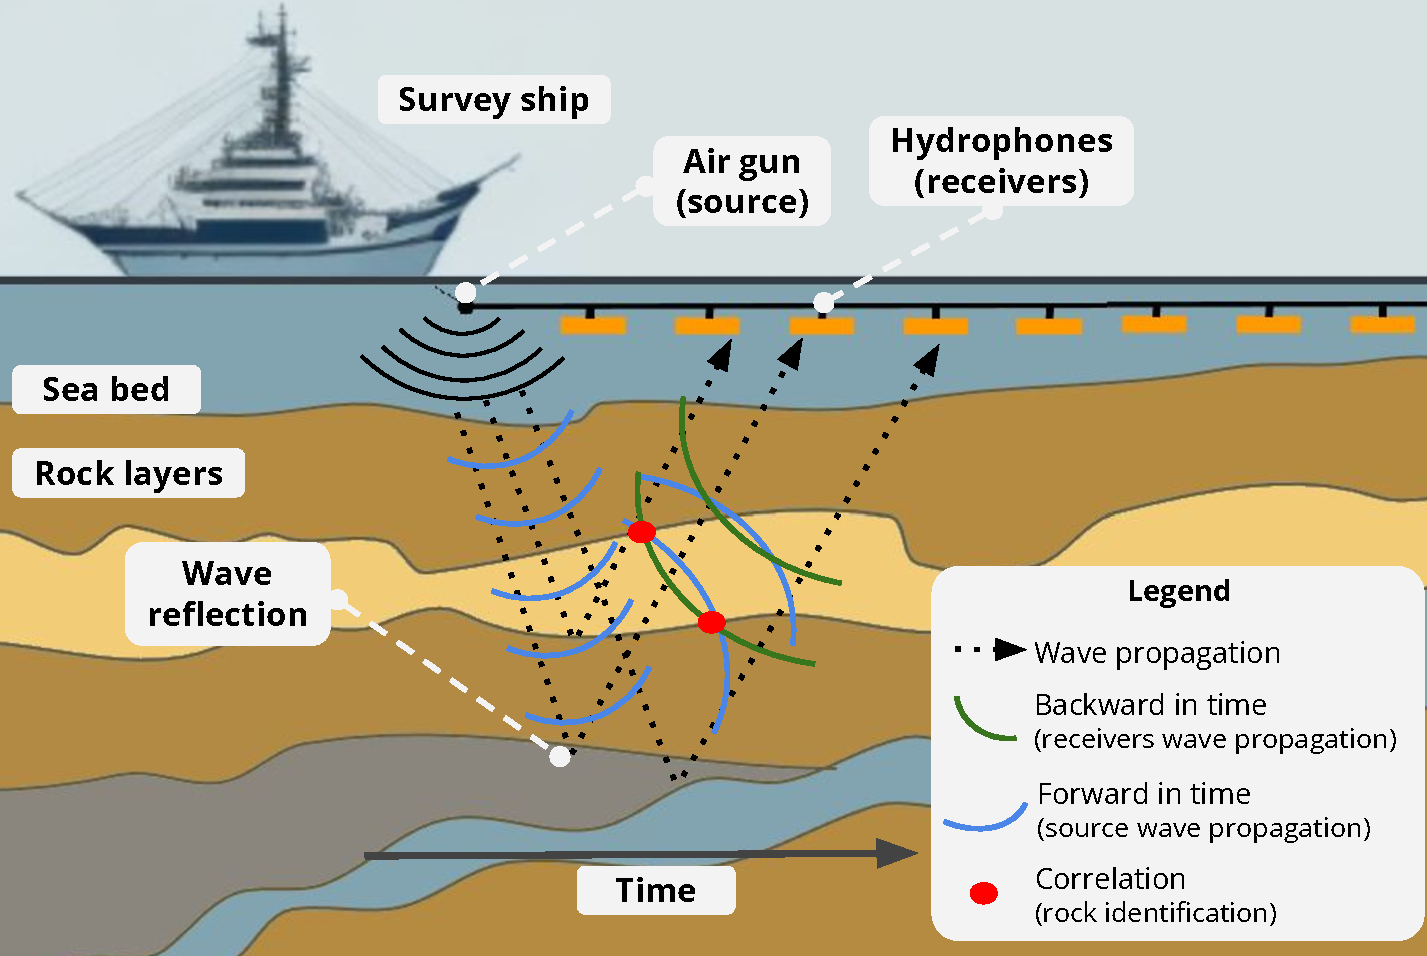
\includegraphics[width=0.75\textwidth]{figures/rtm.pdf}
    \caption[Seismic survey]{Seismic survey process. Blue arcs represent forward wave propagation, green arcs represent backward propagation, and red dots indicate crosscorrelation points.}
    \label{fig:rtm}
\end{figure}

To accurately reconstruct the subsurface, seismic data undergoes \tit{migration}, a process that corrects distortions caused by variations in wave velocity across different geological layers. Migration repositions reflectors at their true depths, converting seismic recordings into interpretable structural images. Several migration techniques exist, each with specific trade-offs, including Kirchhoff Migration, Beam Migration, One-Way Wave Equation Migration (OWEM), and Reverse Time Migration (RTM)~\cite{etgen2009}.

Reverse Time Migration (RTM), introduced by Baysal \etal in 1983 \cite{rtm}, is widely recognized as one of the most accurate migration methods, particularly for complex geological structures with steep dips and strong velocity contrasts. Compared to Kirchhoff and Beam Migration, RTM better handles wavefield multipathing and sharp velocity changes. However, this accuracy comes at a significant computational cost due to its reliance on full wavefield propagation and time-reversal techniques. RTM's imaging quality compared to other methods may be found in~\cite{etgen2009}, Figure 6.


% \section{Reverse Time Migration (RTM)}
% \label{sec:rtm}



RTM operates iteratively over multiple \textit{shots}, each representing the propagation of waves from a single seismic source to the receivers (see dotted lines in Figure~\ref{fig:rtm}). The wave equation is solved for each shot over a series of discrete time steps to model wave propagation. To do this, the continuous wave equation is discretized using the Finite Difference Method (FDM), which represents space and time as a structured computational grid. In this numerical approach, the wavefield at each grid point is updated iteratively based on values from previous time steps \cite{etgen2009}.

Once the wave equation is discretized, the RTM process unfolds in two main phases. In the \textbf{Forward Phase}, the wavefield is computed forward in time from the source location (see ~\rfig{rtm}, blue arches). Then the \textbf{Backward Phase} begins; here, the recorded seismic data is injected at receiver positions and propagated in reverse time (see \rfig{rtm}, green arches). At each step, the backward-propagated wavefield is cross-correlated with the stored forward wavefield to construct the final migrated image (see \rfig{rtm}, red dots)\cite{etgen2009}.

The cross-correlation step presents a computational challenge beyond the inherent cost of solving the wave equation with FDM: both forward and backward wavefields must be available in memory simultaneously. Storing full wavefield snapshots requires substantial memory, making large-scale RTM computations impractical without optimization. To address this, researchers have developed strategies such as wavefield reconstruction from boundary conditions and \checkpointing methods, which aim to reduce storage requirements while preserving computational accuracy~\cite{dussand2008, symes2007}.



\section{Checkpointing}
\label{sec:chkpt}

As introduced in \rssec{rtm}, one of the challenges in RTM computation is ensuring that the results from a given timestep in the forward computation are available during the backward phase for cross-correlation. A naive approach to address this challenge is presented in \ralg{rtm_naive1}, where each timestep in the backward phase recomputes the forward phase entirely, resulting in an algorithm with $\mathcal{O}(\textit{timesteps}^2)$ complexity~\cite{symes2007}; which highly inefficient in terms of processing time, although storage-friendly since it discards the forward data after backward computation and cross-correlation.

\begin{algorithm}[H]
\caption{Naive forward and backward phases with cross-correlation. Algorithm complexity: $\mathcal{O}(\textit{timesteps}^2)$.}
\label{alg:rtm_naive1}
\begin{algorithmic}[1]  % [1] enables line numbering
\STATE Initialize bwdData;
\FOR{$tsBwd = timesteps - 1$; $tsBwd \geq 0$; $tsBwd = tsBwd - 1$}
    \STATE Initialize fwdData;
    \FOR{$tsFwd = 1$; $tsFwd \leq tsBwd$; $tsFwd = tsFwd + 1$}
        \STATE ComputeForward(fwdData, tsFwd);
    \ENDFOR
    \STATE ComputeBackward(bwdData, tsBwd);
    \STATE Crosscorrelate(fwdData, bwdData);
    \State Free(fwdData);
\ENDFOR
\end{algorithmic}
\end{algorithm}

To reduce the algorithm complexity, the program could run the forward loop once and save all results (snapshots) for later cross-correlation during the backward phase, which is impractical due to memory constraints. For instance, the result of a single iteration of the Marmousi3D dataset requires approximately $500MB$, with $6,751$ timesteps, the total storage demand would exceed $3.2TB$, making it infeasible. Even if larger storage solutions like HDDs or SSDs were used, the overhead of transferring data could be more costly than recomputing it on accelerators like GPUs.

To address this, \checkpointing aims to balance the extremes of full recomputation and full storage, optimizing memory consumption while minimizing redundant computations. The effectiveness of each technique depends on factors like memory availability and hardware constraints \cite{symes2007}.

Beyond defining the ideal number of snapshots and recomputation needed to solve the problem, \checkpointing algorithms orchestrate what and when the timesteps should be processed backward and forward, and when a checkpoint should be taken or restored. To simplify the understanding, this dissertation provides a unified terminology: \fwd (compute forward), \save (store a checkpoint), \restore (re-materialize a checkpoint), and \bwd (compute the backward).

\rfig{checkpointing} illustrates \checkpointing in action with only five timesteps. Initially, at \circled{1}, the process computes forward through timesteps, saving snapshots \tinycircled{C1} and \tinycircled{C2}. The forward computation continues until \ttt{t5}, after which backward computation begins using available forward-phase data.

At \circled{2}, if no \checkpointing were used, the entire forward computation from \ttt{t1} to \ttt{t4} would need to be recomputed. However, checkpoint \tinycircled{C2} allows the re-materialization of \ttt{t3}, then only recomputation of \ttt{t4} is required, avoiding redundant calculations. The process continues similarly with snapshots \tinycircled{C1} and \tinycircled{C2}.

Without \checkpointing, this example would require 15 forward computations, while with \checkpointing, only 7 are needed, highlighting the method's effectiveness in reducing redundant work.

\begin{figure}
    \centering
    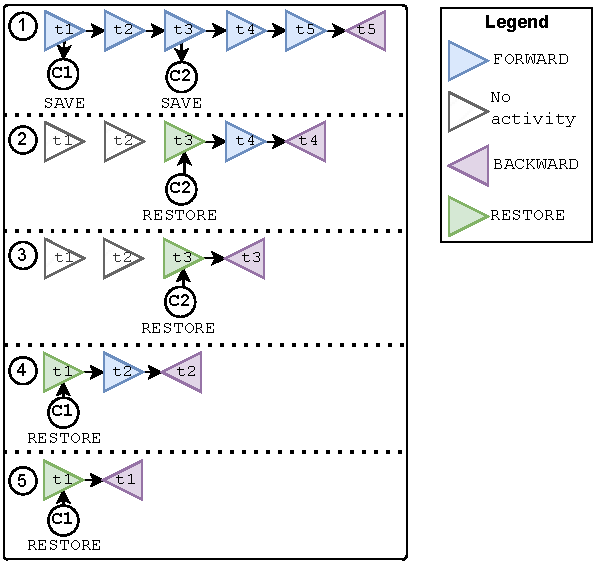
\includegraphics[width=0.6\linewidth,clip]{figures/checkpointing.pdf}
    \caption[Checkpointing timeline]{Example of forward and backward checkpointing in adjoint computation with five timesteps and two snapshots.}
    \label{fig:checkpointing}
\end{figure}
 
This dissertation concentrates on three \checkpointing algorithms: \revolve \cite{revolve}, \uniform, and \zcut \cite{zcut}; however, the goal of this research is not to determine the best algorithm but to demonstrate that the techniques implemented in \gpuzip are adaptable across different \checkpointing approaches. The three \checkpointing algorithms used are:

\begin{itemize}
    \item \textbf{\revolve} \cite{revolve} is a well-established \checkpointing algorithm, originally proposed in 1992 \cite{revolve1992} and later implemented as a C-library in 2000 \cite{revolve}. Even after three decades, it remains widely used, for instance, in the \tit{Devito Framework} \cite{devito-api, devito-compiler}, a popular open-source toolbox for finite difference problems, image processing, and machine learning. 
    
    \revolve optimizes the problem presented in \ralg{rtm_naive1}, reducing its complexity to $\mathcal{O}(n \log n)$. It follows a \tit{bisection-based \checkpointing} strategy, where the total number of snapshots, is determined as $\log_4 (\text{timesteps})$. 

    The algorithm begins by performing \fwd computation, periodically saving a checkpoint every $(\frac{timesteps} {snaps})$ steps. Once \bwd computation starts, it restores the nearest available checkpoint and reprocesses \fwd up to the required \bwd timestep. Once \bwd timestep is the same as the last checkpoint saved, the checkpoint will not be used anymore -- letting space to take one more checkpoint. This enables \revolve to iteratively restore the closest checkpoint, recompute \fwd, and strategically place additional snapshots along the way. As more checkpoint slots become available, additional snapshots can be stored, avoiding more computation.

    \item \textbf{\uniform} is a straightforward \checkpointing strategy that takes snapshots evenly across the execution timeline. The user defines the maximum number of snapshots based on available memory, and the algorithm calculates uniform intervals for saving and restoring them. For example, in a simulation with 6,751 timesteps and a storage capacity for $100$ snapshots, \uniform would place a checkpoint approximately every $67$ timesteps. The \uniform algorithm used in this work is an in-house developed code; however, the idea of ``uniformly spaced \checkpointing'' is not a novelty \cite{ahlroth2011}.

    \item \textbf{\zcut}\cite{zcut} algorithm tackles the problem by representing it as a directed acyclic graph, known as a computational graph. In this graph, nodes represent computational tasks (kernels), and edges show the data dependencies between these tasks. It determines which nodes should be saved. The nodes not saved during the forward phase must be recomputed from the most recent checkpoint during the backward phase. \zcut takes snapshots for all nodes for a given interval of execution, then after this chunk is completed, the nodes are discarded and moves to the next chunk.
\end{itemize}


Despite their differences and trade-offs, \revolve, \zcut, and \uniform share common traits. They are deterministic, ensuring identical inputs produce the same checkpoint sequence. Additionally, all three rely on a structured control loop to dictate execution steps: \fwd, \save, \restore, \bwd, and \terminate, making them systematic and predictable solutions for large-scale adjoint computations. 

% \begin{algorithm}[H]
% \caption{High-level Control Loop for the RTM application}
% \label{alg:controlloop}
% \begin{algorithmic}[1]  % [1] enables line numbering
%     \STATE $iteration \gets 0$
%     \REPEAT
%         \STATE $action, timestep \gets \text{GetAction()}$
%         \IF{$action$ is \fwd}
%             \STATE $\text{computeForward}(timestep)$
%         \ELSIF{$action$ is \save}
%             \STATE $\text{saveCheckpoint}(timestep)$ \COMMENT{DeviceToHost}
%         \ELSIF{$action$ is \restore}
%             \STATE $\text{restoreCheckpoint}(timestep)$ \COMMENT{HostToDevice}
%         \ELSIF{$action$ is \bwd}
%             \STATE $\text{computeBackward}(timestep)$
%         \ENDIF
%         \STATE $iteration \gets iteration + 1$
%     \UNTIL{$action$ is not \terminate}
% \end{algorithmic}
% \end{algorithm}



\section{Hegerogeneous Computing Systems \& GPUs} %or computer architecture?%
\label{sec:gpus}

Over the last two decades, the semiconductor industry and the field of computer science have increasingly focused on parallel computing architectures to address the growing demand for high-performance computing~\cite{hennessy}. For numerically intensive applications like Reverse Time Migration (RTM), which rely heavily on floating-point operations, heterogeneous computing systems that combine traditional CPUs with accelerators like GPUs or FPGAs have become widely adopted \cite{dussand2008,liu2012,rigon2024}.

GPUs have emerged as massively parallel devices capable of achieving impressive performance. For instance, an NVIDIA V100 GPU can reach up to $15.7$ teraflops in FP32 and $7.8$ teraflops in FP64\cite{v100}. At the same time, newer architectures like the NVIDIA A100 push the limit to $19.5$ teraflops in FP32~\cite{a100}. In contrast, a high-end CPU like the Intel Xeon Gold 6240 delivers around $0.921$ teraflops~\cite{xeon}. This raw comparison suggests a potential $15\times$ performance gap, but each processor is designed for a different goal: CPUs are optimized for low-latency sequential tasks, while GPUs prioritize high-throughput parallelism~\cite{kirk}.

To better understand this distinction,~\rfig{gpu} illustrates a typical heterogeneous computing system composed of a GPU (``Device'') and a CPU (``Host'') connected via the PCIe bus. While CPUs consist of a few cores, each with its own control, cache, and ALU (Arithmetic Logic Unit), the GPU consists of thousands of ALUs, allowing it to process many threads simultaneously. For example, the NVIDIA V100 features 5120 FP32 cores and 2560 FP64 cores~\cite{v100}. This dense arrangement of ALUs and the GPU's access to high-bandwidth memory (HBM2) enables it to perform floating-point arithmetic much faster than CPUs~\cite{kirk}.

\begin{figure}[h!]
    \centering
    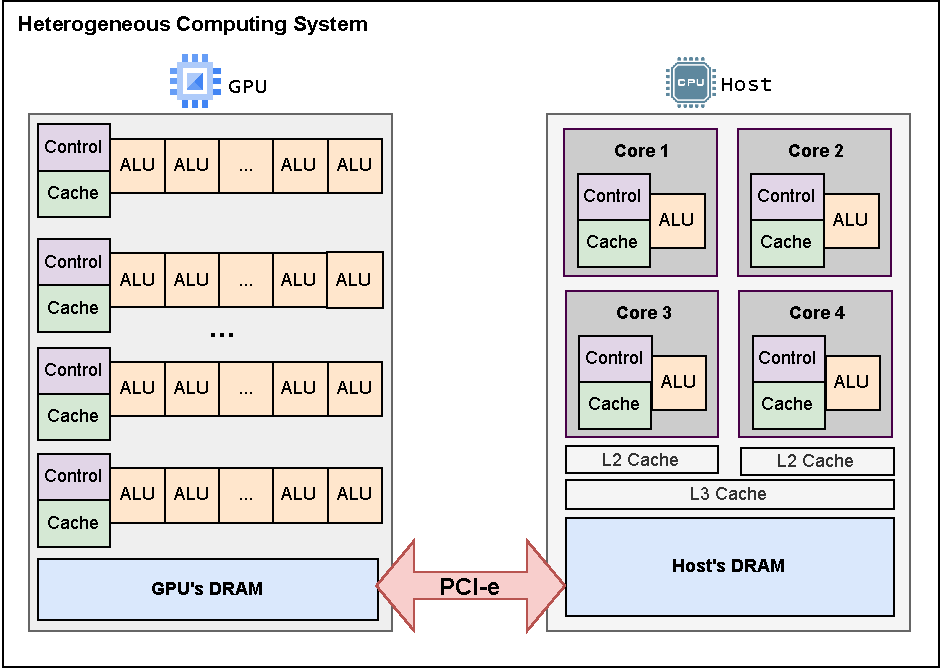
\includegraphics[width=0.8\linewidth,clip]{figures/gpu.pdf}
    \caption[System with GPU and CPU diagram]{Diagram of a Heterogeneous Computing System composed of a GPU and CPU.}
    \label{fig:gpu}
\end{figure}

GPUs' high throughput stems from their ability to exploit massive parallelism through the SIMT (Single Instruction, Multiple Threads) execution model. SIMT shares some characteristics with SIMD (Single Instruction, Multiple Data; from Flynn's taxonomy), as both allow the execution of the same instruction across multiple data elements. However, SIMT differs by combining this parallelism with independent thread control, allowing not only arithmetic operations but also control flow and branching logic within each thread\cite{cuda}.

GPUs are managed by programming models such as OpenCL or NVIDIA's CUDA. Both support the C/C++ environment and have their own directives and extensions to allow the development of programs that use GPUs~\cite{kirk}. This dissertation concentrates on the CUDA programming model.

CUDA introduces two essential concepts: thread blocks and grids. A group of threads is called a ``thread block'' and can work together using fast on-chip shared memory and synchronize with each other. A grid is formed by collecting these thread blocks covering the entire input data~\cite{cuda}.

From the programmer's perspective, CUDA separates code that runs on the host (CPU) from code that runs on the device (GPU). CUDA kernels are functions marked with the \ttt{\_\_global\_\_} keyword launched from the host and executed in parallel on the GPU. The example in~\rlst{cudaexample} shows a simple kernel that adds two vectors element-wise.

\begin{figure}[h]
\centering
\begin{lstlisting}[language=C++, caption={CUDA kernel and host code for element-wise vector addition. This is an adapted version from the example given in Hwu, Wen-Mei W~\etal(2022)\cite{kirk}}, label={lst:cudaexample}]
__global__ void vecAddKernel(float *a, float*b, float*c, int n) {
    int i = threadIdx.x + blockDim.x * blockIdx.x;
    if (i < n) {
       c[i] = a[i] + b[i];
    }
}

main() {
   float *A_h, *B_h, *C_h;

   int na = readFile(&A_h, "./a.bin"); // returns vector size
   int nb = readFile(&B_h, "./b.bin"); // returns vector size

   if (na != nb) { fprintf(stderr, "Array size mismatch\n"); return 1;}

   int n = n_a;
   int size = n * sizeof(float);
   C_h = (float *)malloc(size);
 
   cudaMalloc((void **) &A_d, size);
   cudaMalloc((void **) &B_d, size);
   cudaMalloc((void **) &C_d, size);

   cudaMemcpy(A_d, A, size, cudaMemcpyHostToDevice);
   cudaMemcpy(B_d, B, size, cudaMemcpyHostToDevice);

   vecAddKernel<<<ceil(n/256.0), 256>>>(A_d, B_d, C_d, n);

   //C_h can be used by the host after d2h. C_d is used only in GPU.
   cudaMemcpy(C_h, C_d, size, cudaMemcpyDeviceToHost);

   cudaFree(A_d); cudaFree(B_d); cudaFree(C_d);
   free(A_h);free(B_h);free(C_h);
}
\end{lstlisting}
\end{figure}

The host code handles memory allocation (\ttt{cudaMalloc}), data transfer (\ttt{cudaMemcpy}), and invokes kernel using the triple angle bracket syntax to run in the device: \sloppy{\verb|<<<blocks, threads>>>| ~\cite{cuda}}. For example, with $n = 1000$ and $256$ threads per block, the launch configuration \sloppy{\verb|<<<4, 256>>>|} creates $1024$ threads. The extra 24 threads are discarded using the guard condition \sloppy{\verb|if (i < n)|} inside the kernel~\cite{kirk}.

CUDA also allows device memory allocation and data movement between the host and the device~\cite{cuda}. In the example from~\rlst{cudaexample}, memory allocations occur in lines 20–22, \htd transfers in lines 24–25, and the result is copied back to the host (\dth) in line 30. These operations are synchronous by default, meaning the GPU must wait idle during transfers.

Even though GPUs have impressive FLOPS capacity and potential for massive parallelism, developing applications for heterogeneous computer systems can be challenging. One significant hurdle is the high latency communication between devices, which can shatter the dreams of accelerating applications with GPUs~\cite{kirk,cuda,liu2012}. 

As illustrated in~\rfig{gpu}, \dth and \htd communication happens over the PCIe bus\cite{kirk}, which is much slower than accessing GPU-local memory. For instance, NVIDIA v100 (with PCIe 3.0) offers a host-device bandwidth of $32 GB/s$, while access to HBM2 memory (GPU's DRAM) achieves $900 GB/s$ --- a staggering $28\times$ difference~\cite{v100}.

CUDA provides asynchronous data transfer mechanisms to minimize idle time using \ttt{cudaStream}. With \ttt{cudaMemcpyAsync}, data transfer can occur concurrently with kernel execution, since they are assigned to different \ttt{cudaStreams}. CUDA offers synchronization mechanisms like \ttt{cudaStreamSynchronize} to control execution without blocking all streams as \ttt{cudaDeviceSynchronize} would~\cite{kirk,cuda}.

In summary, parallel programming accelerators offer significant opportunities to accelerate applications. However, as Amdahl's laws suggest~\cite{hennessy}, programmers must know when and how to use them to accelerate their programs, and which part of the program, respecting the system and the application's requirements and limitations.

\section{\awave}
\label{sec:awave3d}

\awave is a Reverse Time Migration (RTM) implementation that solves 3D fields. It was developed through a collaborative effort between the Faculty of Geophysics\footnote{\url{https://cpgf.propesp.ufpa.br/index.php/en/} - Accessed May 26, 2025} at Pará Federal University (UFPA), the Institute of Mathematics, Statistics and Scientific Computing (IMECC)\footnote{\url{https://www.ime.unicamp.br/en} - Accessed May 26, 2025}, and the Institute of Computing (IC)\footnote{\url{https://ic.unicamp.br/en/} - Accessed May 26, 2025} at Unicamp. It was designed as a research-oriented platform to explore and advance computational strategies for seismic imaging and wavefield modeling.

\awave supports a variety of computational flavors tailored to different levels of hardware complexity and parallelism: CPU-only; GPU (single device); \textbf{SNMG} – \textit{Single-Node Multi-GPU}, which decomposes the wavefield across multiple GPUs on the same machine; and \textbf{MNMG} – \textit{Multi-Node Multi-GPU}, which extends SNMG and distributes shots across nodes using intra-node GPU decomposition.

All these versions incorporate \checkpointing, initially powered by the \revolve algorithm, to optimize memory usage during wavefield reconstruction. For this work, however, \awave was refactored to support interchangeable \checkpointing libraries, as~\rch{oss} will discuss further.

The storage used for \checkpointing data in \awave is organized as shown in \rfig{baseline}: when a \save \circled{1} operation occurs, data is transferred from GPU memory to host memory (\dth). Then, during a \restore \circled{2} operation, data is fetched back from host memory to GPU memory (\htd).

\begin{figure}[h!]
    \centering
    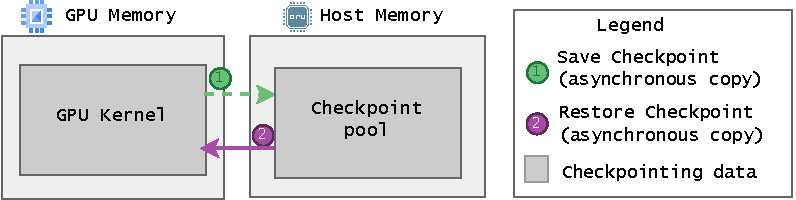
\includegraphics[width=1\linewidth,clip]{figures/arch_baseline.pdf}
    \caption[\awave baseline memory architecture diagram]{Baseline memory architecture for \checkpointing in \awave.}% Every \save the data is sent to the host memory, and every \restore the data is transferred from the host to the GPU memory.}
    \label{fig:baseline}
\end{figure}

In SNMG, the computational domain is spatially decomposed across multiple GPUs. Each GPU handles a portion of the wavefield using the following CUDA kernels:
\begin{itemize}
  \item \texttt{InjectionForward}: injects the seismic source into the forward wavefield.
  \item \texttt{UpdateForward}: propagates the wavefield forward in time using finite-difference stencils.
  \item \texttt{InjectionBackward}: injects the receiver wavefield into the backward propagation pass.
  \item \texttt{UpdateBackward}: performs the time-reversed propagation for imaging.
\end{itemize}
This spatial decomposition allows each GPU to compute its subdomain while exchanging boundary information with neighboring GPUs as needed.

The MNMG flavor builds on SNMG but distributes the \textit{shots} across multiple compute nodes. It is implemented using \textbf{OpenMP Cluster (OMPC)}~\cite{ompc}, a library developed by researchers at the Computer Systems Laboratory (LSC)\footnote{\url{https://lsc.ic.unicamp.br/} - Accessed May 26, 2025}. OMPC allows OpenMP directives to distribute work across nodes via MPI, but the MPI layer is transparent from the programmer's perspective.

\awave uses OMPC directives to distribute the shots through the worker nodes from the central node (using \sloppy{\verb|#pragma omp parallel|}). Then it dispatches data using \sloppy{\verb|#pragma omp target nowait map(to:...)|}\footnote{\url{https://ompcluster.readthedocs.io/en/latest/programming.html\#asynchronous-target-task} -- Accessed May 26, 2025}\footnote{\url{https://ompcluster.readthedocs.io/en/latest/programming.html\#manage-the-device-data-environment} -- Accessed May 26, 2025}. Each node then executes the SNMG-style decomposition. At last, a node synchronization happens to consolidate the final results, generating the migrated image.


\chapter{ Related Work }
\label{ch:related_work}

%This chapter reviews the relevant literature on the techniques discussed in this dissertation. GPUZIP introduces a novel approach by integrating GPU-based lossy \compression with \prefetching checkpoint data from the host to GPU memory. It works seamlessly with different \checkpointing algorithms and allows for exploring prefetching and \compression parameters to fine-tune the checkpoint mechanism to specific application profiles. Prior research has typically treated \compression and \prefetching as distinct processes, often using different methodologies or focusing on other objectives.

This chapter reviews the relevant literature on the techniques discussed in this dissertation. GPUZIP introduces a novel approach by integrating GPU-based lossy \compression with \prefetching checkpoint data from the host to GPU memory. It works seamlessly with different \checkpointing algorithms and allows users to fine-tune through compression and prefetching parameters. Prior research has typically treated \compression and \prefetching as distinct processes, often using different methodologies or focusing on other objectives.

This chapter is organized as follows: \rsec{review} presents a review of the relevant literature related to this work, while \rsec{thiswork} distinguishes features of the proposed approach.



\section{Literature Review}
\label{sec:review}

Lossy \compression has become an important tool in scientific computing, particularly for applications like Reverse Time Migration (RTM), where data volumes are large and memory or I/O bandwidth is limited~\cite{cappello2025,di2025}. Literature uses \compression techniques executed on CPUs or GPUs (or both) to help reduce storage requirements, enabling more snapshots to be stored and lower communication overhead, for example, device-host memory or memory-disk transfers.

Margetis~\etal(2021, 2023)~\cite{margetis2021,margetis2023} applied CPU-side lossy \compression to store more wavefield snapshots, thereby reducing recomputation. Similarly, Huang~\etal(2023)\cite{huang2023} introduced a CPU-based framework that compresses forward wavefields after each timestep and decompresses them during backward propagation. Their work significantly reduces I/O time and storage needs, achieving up to $6.6\times$ speedup by alleviating the I/O bottleneck in checkpoint-like workflows.

%Several studies have explored CPU-based \compression strategies to optimize memory and storage. Margetis~\etal(2021, 2023)~\cite{margetis2021,margetis2023} applied CPU-side lossy \compression to store more wavefield snapshots, thereby reducing recomputation. 

%Similarly, Huang~\etal(2023)\cite{huang2023} introduced a CPU-based framework that compresses forward wavefields after each timestep and decompresses them during backward propagation. Their work significantly reduces I/O time and storage needs, achieving up to $6.6\times$ speedup by alleviating the I/O bottleneck in checkpoint-like workflows.

GPU-based approaches have also been adopted in the reviewed literature. Kukreja~\etal(2020)\cite{kukreja2020} showed that GPU \compression can accelerate solvers by enabling more checkpoint data to be stored in limited GPU memory. Dmitriev~\etal(2022)\cite{dmitriev2022} employed cuZFP and NVIDIA Bitcomp (also used in this dissertation) to compress seismic data while preserving imaging quality. Barbosa and Coutinho~(2023)\cite {barbosa2023} compared lossy and lossless \compression in RTM, demonstrating substantial reductions in wavefield storage and I/O overhead. Shen~\etal(2022, 2023)\cite{shen2022,shen2023} further explored GPU-based \compression to mitigate data transfer bottlenecks between host and GPU; their research resulted in $2.09\times$ of speedup on FP32 data and could reduce GPU memory usage by 21\%.

Maurya~\etal(2023b)\cite{maurya2023compress} proposes a pipeline of accumulated GPU data \compression before transferring the data to the host memory. Their work also uses NVIDIA Bitcomp lossy \compression and uses an RTM implementation as a case study, as presented in this dissertation.

In the context of \tit{Prefetching}, the literature defines it as a latency-hiding technique where data is proactively retrieved from slower memory (e.g., main memory or disk) and placed into faster memory (e.g., CPU cache or GPU memory) before it is needed\cite{mittal2017,vanderwiel2000}. The literature is extensive on the applications in which this technique can be applied and how it is implemented, for example, what devices are involved, runtime or compiling time, what architecture is concerned, if it is implemented in hardware or software, etc. This dissertation concentrates on analyzing related work in the context of prefetching data from the host memory to the GPU memory for seismic data or prefetching checkpoint data.

Some works introduce the concept of asynchronous copy from the host memory to the GPU memory~\cite{jeong2022,jung2020}. Even though those works do not propose a prefetch algorithm based on data access patterns, asynchronous copies that hide communication latency inspired our research. In the context of seismic data, Rigon~\etal(2024)~\cite{rigon2024} improved performance by up to 62\% through asynchronous prefetching and Unified Memory optimizations, highlighting the benefit of preloading data from host to GPU, even though their work did not specifically target \checkpointing.

Regarding prefetching of checkpoint data, Maurya~\etal (2023a)~\cite{maurya2023} proposed a multilevel storage prefetching mechanism on the VeloC\footnote{\url{https://veloc.readthedocs.io/} - accessed May 26, 2025} checkpoint library, that provides a multi-level checkpoint-restart runtime. It is worth noting that VeloC is not the same as \revolve or \zcut, which define when a checkpoint is taken, but the user specifies when it should take the snapshot or be materialized. Based on VeloC's premises, their work prefetches data in a multi-level fashion, defining hints on when a checkpoint should be prefetched from a lower level, i.e., CPU memory, to a higher level, i.e., GPU memory. Their work also uses an RTM implementation as a case study. 


% GPUZIP takes a different approach by planning prefetch actions—before solver execution—allowing it to work agnostically with different checkpointing algorithms, regardless of when \save or \restore operations occur.

\section{This work}
\label{sec:thiswork}

%GPUZIP proposes communication optimization in GPU-based adjoint/reverse with \checkpointing by combining checkpoint prefetching and lossy data \compression on the GPU side. It introduces a \psa, a predictive prefetching mechanism that anticipates cache raw misses and schedules the asynchronous retrieval of checkpoint data from the host to GPU memory ahead of time. GPUZIP applies GPU-based lossy \compression to checkpoint data already residing in GPU memory, reducing the volume of data transferred over PCIe. The prefetching and \compression techniques are modular and can be used independently or in combination, providing flexible configuration through the GPUZIP API.

GPUZIP proposes communication optimization in GPU-based adjoint/reverse solver implementations with \checkpointing by combining checkpoint prefetching and lossy data \compression on the GPU side. It introduces a checkpoint cache system and a prediction algorithm that is capable of avoiding cache misses by scheduling anticipated asynchronous retrievals of checkpoint data from the host to GPU memory ahead of time. GPUZIP applies GPU-based lossy \compression to checkpoint data already residing in GPU memory, reducing the volume of data transferred over PCIe. The prefetching and \compression techniques are modular and can be used independently or in combination, providing flexible configuration through the GPUZIP API.

One of the key features of GPUZIP is its ability to integrate with existing \checkpointing libraries seamlessly. It accomplishes this by wrapping these libraries and conducting a dry-run simulation, which generates an optimized prefetch schedule. This functionality has been tested with multiple \checkpointing strategies across various deterministic algorithms, including \revolve, \zcut, and \uniform.

While many prior works have explored \prefetching or \compression independently, fewer studies combine both techniques in the context of \checkpointing. Maurya \etal (2023a)\cite{maurya2023} proposed a system incorporating \prefetching and \compression, leveraging the VELOC library. Their work addresses heterogeneous memory hierarchies and schedules data movement across storage tiers, including network storage, SSDs, host DRAM, and GPU memory. Although their architecture includes \compression in the pipeline (as shown in Figure 3 of their paper), it does not isolate the impact of \compression versus prefetching, nor does it explain how their prefetching mechanism would behave in the absence of \compression.

Furthermore, VeloC, while a robust general-purpose \checkpointing framework, does not implement an algorithm designed explicitly for reverse-mode or adjoint computations, such as \revolve or \zcut. In VeloC, the responsibility for defining when to save or restore checkpoint data is left to the user.

Although a direct performance comparison would be valuable, the binaries or source code for Maurya \etal prefetching mechanism are not publicly available, preventing a direct evaluation against GPUZIP.


\chapter{Prefetching Checkpoint Data}
\label{ch:prefetch}

Prefetching is a well-established technique in computer systems that improves performance by proactively fetching data from slower to faster storage tiers, thereby minimizing latency and avoiding execution stalls~\cite{mittal2017,vanderwiel2000}. It can be implemented at both the hardware and software levels. At lower architectural levels, prefetching is commonly employed in CPU cache systems (L1, L2, L3) to preload data and instructions~\cite{mittal2017,emma2005,hennessy}. At higher levels, within applications, it is used to preload data from disks into DRAM~\cite{patterson1995,butt2007}, and to manage multi-level memory hierarchies where data is staged from disk to host memory and ultimately to GPU memory~\cite{maurya2023}. The main advantage of prefetching is to ensure that data is available precisely when needed, thus reducing delays caused by slow memory transfers.

Prefetching mechanisms typically rely on \textit{hinting}, where an algorithm either recognizes memory access patterns or has prior knowledge of future data requirements~\cite{patterson1995, maurya2023}. When prefetching is implemented, a caching or buffering mechanism is often required~\cite{patterson1995, butt2007, maurya2023} to store prefetched data temporarily until it is accessed.

The implementation complexity of a caching mechanism depends on the system's characteristics and application. If prefetched data is guaranteed not to be overwritten, minimal control is required. However, if storage must compete with other processes or memory constraints, replacement policies such as Least Recently Used (LRU) and Most Recently Used (MRU) become essential~\cite{butt2007, carr1981}.

The idea behind \checkpointprefetching in this research is to transfer checkpoint data from host memory to GPU memory in advance. The goal is to alleviate the bottleneck of synchronous copying between host and GPU memories.

This dissertation adopts terminology similar to Emma~\etal (2005)\cite{emma2005} and Ho~\etal (2025)\cite{ho2025}, standardizing concepts and facilitating evaluation. First, \textit{raw misses} refer to cache misses that would occur without prefetching, while \textit{misses} denote the actual cache misses that happen during execution with prefetching; a \tit{real hit} is when the data is already in the cache but no prefetch was needed and \tit{hit} is when the checkpoint is in the cache at the moment it need to be used. \tit{Timely prefetches} are the ones could finish their transfers before their usage, and \tit{late prefetches} refers to the ones could not be copied in time before their usage (opposite to timely prefetches). Finally, \textit{timeliness} describes the time interval between initiating a prefetch and its actual use, which determines whether the data is available just in time.

%Emma~\etal(2005)\cite{emma2005} introduced a prefetching terminology adopted in this work to standardize concepts and facilitate evaluation. First, prefetches are categorized as either \textit{good} or \textit{bad}: a prefetch is considered good if the data is used before it is evicted from the cache; otherwise, it is classified as bad. \textit{Raw misses} refer to cache misses that would occur without prefetching, while \textit{misses} denote the actual cache misses that happen during execution with prefetching. Finally, \textit{timeliness} describes the time interval between initiating a useful prefetch and its actual use, which determines whether the data is available just in time.

%Emma~\etal(2005)\cite{emma2005} introduced a prefetching terminology adopted in this work to standardize concepts and facilitate evaluation. First, prefetches are categorized as either \textit{good} or \textit{bad}: a prefetch is considered good if the data is used before it is evicted from the cache; otherwise, it is classified as bad. \textit{Raw misses} refer to cache misses that would occur without prefetching, while \textit{misses} denote the actual cache misses that happen during execution with prefetching. The \textit{coverage} metric quantifies the proportion of raw cache misses successfully handled by good prefetches, defined as the ratio of good prefetches ($G$) to total raw misses ($M$). \textit{Accuracy} is the fraction of prefetches that are good among all issued prefetches; low accuracy may increase unnecessary data movement and degrade performance. Finally, \textit{timeliness} describes the time interval between initiating a useful prefetch and its actual use, which determines whether the data is available just in time.

% While the primary goal of GPUZIP’s prefetching mechanism is to improve end-to-end performance, its internal success is determined by prefetch efficiency. Ideally, the number of \tit{raw misses} should exceed the number of observed \tit{misses}, indicating that Prefetching is not causing misses and degrading performance; also prefetching the blocking time spent of a raw miss should not exceed the blocking time of a prefetched checkpoint, in other words, prefetches must be issued with sufficient \textit{timeliness} to hide data transfer latency; that is,
% \[
% T_{\text{timeliness}} > T_{\text{h2d}}
% \]
% where $T_{\text{h2d}}$ is the time to transfer a checkpoint from host to device memory.

While this research's prefetching mechanism is designed to improve end-to-end performance, its effectiveness also depends on internal efficiency. One key indicator of this efficiency is the relationship between \textit{raw misses} (misses that would occur without prefetching) and actual \textit{misses} observed during execution. Ideally, the number of raw misses should be greater than the number of observed misses, indicating that prefetching effectively reduces the frequency of cache misses rather than introducing new ones.

In addition, the blocking time associated with a raw miss should not be greater than the blocking time of prefetching it. In other words, a prefetch must be issued with sufficient \textit{timeliness} to hide the data transfer latency. This can be expressed as:
\[
T_{\text{timeliness}} > T_{\text{h2d}}
\]
where $T_{\text{timeliness}}$ is the time between the prefetch being issued and the checkpoint being consumed, and $T_{\text{h2d}}$ is the time required to transfer the checkpoint from host to device memory.

This chapter is organized as follows: \rsec{prefetch_methodology} describes the prefetching mechanism, its components, and how it integrates into \awave. And then, \rsec{prefetch_result} presents the experimental results of the adopted technique in different datasets, \checkpointing algorithms, and configurations.


\section{Methodology}
\label{sec:prefetch_methodology}

This section is organized into three subsections. First, \rssec{gpuzip_prefetch} introduces the main components of GPUZIP’s prefetching mechanism and explains how they interact within the context of the \awave RTM implementation. Next, \rssec{caching} provides a detailed explanation of the \cache mechanism, describing its internal structure and behavior. Finally, \rssec{psa} presents the \psa, outlining its steps and how it configures the prefetching process.

\subsection{The Prefetching Mechanism}
\label{sec:gpuzip_prefetch}

The proposed prefetching mechanism leverages the deterministic nature of \checkpointing algorithms by performing a preliminary \textit{Prefetch Setup}. The algorithm does a dry-run execution of the \checkpointing algorithm to predict \save and \restore actions before actual computation begins. The \pav (PAV), which schedules all prefetching operations, is the result of this setup.

Following \rfig{arch_prefetch}, the proposed memory architecture consists of a \cache, where the \checkpointing data is temporarily stored in the GPU memory (discussed further in \rssec{caching}); and the \pool stores all the \checkpointing data in the host memory. All \save and \restore operations communicate directly with the \cache that can retrieve or send data to the \pool in the host memory. The \pav contains the iteration where the prefetch action is dispatched and what snapshot should be moved from the host to the GPU memory.

\begin{figure}[h!]
  \centering
  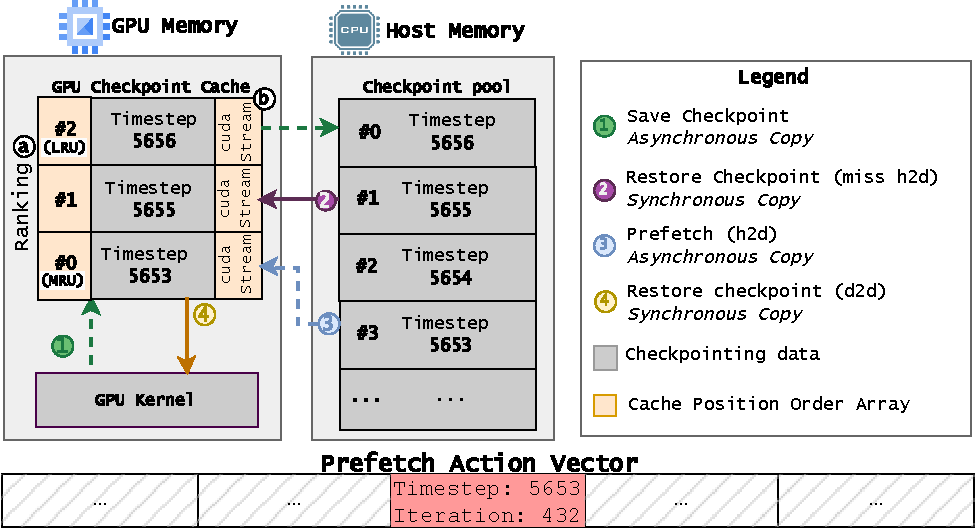
\includegraphics[width=0.9\linewidth,trim={0 0 0 0},clip]{figures/arch_prefetch.pdf}
  % \caption[Memory architecture diagram (\checkpointprefetching)]{GPUZIP's memory architecture with a cache of 3 positions. Every \save the data is stored in the \cache, then the data is asynchronously copied to the \pool in the host. Every \restore with a cache miss, the data is synchronously transferred back to the \cache. Every \restore with a cache hit, the checkpoint is rematerialized from the cache (device-to-device copy). GPUZIP can prefetch the data from the \pool to the \cache asynchronously.}
  \caption[Memory architecture diagram (\checkpointprefetching)]{The prefetching mechanism memory architecture with a cache of 3 positions.}
  \label{fig:arch_prefetch}
\end{figure}

The basic \checkpointprefetching mechanism is explained at a high level through the \ralg{prefetching_loop}, representing the \awave main loop performing actions from the \checkpointprefetching mechanism. The \textit{Prefetch Setup} function (line 1) is the first step to be performed, which will return the PAV. Then, each iteration is checked whether a prefetching action is scheduled in the PAV at the current moment (line 4). If so, the prefetch dispatch method asynchronously transfers data from \htd (line 5) while a \fwd or \bwd computation runs. When a \save operation occurs, GPUZIP first stores the data in the \cache (line 8) before asynchronously saving it to the \pool (line 9). For \restore operations, GPUZIP first checks the cache for the requested checkpoint (line 11). If found, a \textit{cache hit} occurs (line 15), allowing a direct \dtd copy to the necessary data structure. If the data is still being transferred, the system waits for the transfer to complete (lines 12 and 13). If the checkpoint is missing from the cache, the worst-case scenario occurs: a synchronous \htd transfer via PCIe, followed by a \dtd copy to the required location (lines 16-19).

\begin{algorithm}[h!]
\caption{Checkpointing Prefetching Execution Loop}
\label{alg:prefetching_loop}
\begin{algorithmic}[1]
\STATE $pav \gets$ PrefetchSetup($config.cacheSize$)

\WHILE{action $\neq$ TERMINATE}
    \STATE action $\gets$ Checkpointing.GetAction()
    \IF{pav.shouldDispatch()}
        \STATE pav.dispatch()
    \ENDIF
    
    \IF{action == SAVE}
        \STATE Save computing data to cache (D2D)
        \STATE Save from cache to host (D2H)
    \ELSIF{action == RETRIEVE}
        \IF{currentTimestep is in cache}
            \IF{transfer is still happening} 
                \STATE Wait for the transfer to finish
            \ENDIF
            \STATE Copy from cache to computing data (D2D)
        \ELSE
            \STATE Copy from host to cache (H2D)
            \STATE Copy from cache to computing data (D2D)
        \ENDIF
    \ELSIF{action == FORWARD or action == BACKWARD}
        \STATE Perform forward or backward computation
    \ENDIF
\ENDWHILE
\end{algorithmic}
\end{algorithm}


\subsection{The Caching Mechanism}
\label{sec:caching}

Caching is a widely used strategy in computer architecture that allows data to be stored for quick access. Four key questions were considered when designing the caching mechanism for GPUZIP: (A) What should the cache store? (B) How large should the cache be? (C) What is the expected access pattern? And (D) What should happen when the cache is full?

To address question (A), for every \save action, new data should be stored in the cache via a \dtd copy, as illustrated in \circled{1} in \rfig{arch_prefetch}. After this, the checkpoint is asynchronously transferred from the cache to the \pool via a \dth operation. When a \restore~\circled{2} or a prefetching
\circled{3} operation occurs, the checkpoint is loaded into the cache through a \htd copy. The \cache is implemented as a fully associative cache \cite{patterson1995}, meaning that snapshots can be stored in any cache location regardless of their position in the \pool. The fully associative cache is exemplified in \rfig{arch_prefetch}, where the checkpoint at position \ttt{#3} in the \pool is transferred to the position \ttt{#0} in the \cache.

This leads to question (B): How large should the cache be? The \cache must have space for at least two snapshots. When a checkpoint is saved and copied to the \pool, another checkpoint is likely being prefetched into the cache, awaiting imminent use. %While the cache size can be increased if additional GPU memory is available, a minimum of two slots is required for proper functionality.

Regarding access patterns (C), the chosen \checkpointing algorithms likely reuse snapshots shortly after access. For instance, in the \revolve algorithm, the last checkpoint saved during the \fwd phase is the first to be restored during the \bwd phase. Once a checkpoint is retrieved from the cache, it is often needed again because backward computation requires materializing snapshots at multiple stages.

Understanding the access pattern helps answer question (D): When the cache reaches full capacity, an existing checkpoint must be evicted to store the new one. GPUZIP employs a Least-Recently-Used (LRU) replacement policy, meaning the least recently accessed checkpoint is removed to make room for the incoming one, as described in \cite{butt2007}. Whenever a checkpoint is accessed, it is promoted to the Most Recently Used (MRU) position, ensuring that frequently used data remains available.

The \cache includes the \tit{Ranking Controller} (\rfig{arch_prefetch}, \circled{a}) that tracks the order of cached \checkpointing data, mapping their MRU/LRU status to specific GPU memory locations. This eliminates the need for expensive memory allocation, deallocation, or unnecessary data movement when promoting or evicting cache entries. For example, in a three-slot cache (\rfig{arch_prefetch}), if the checkpoint at position \#2 is accessed, it is promoted to MRU (\#0), shifting the previous MRU (\#0) to position \#1, and the previous \#1 to LRU (\#2).

GPUZIP assigns a \ttt{cudaStream} to every cache slot to ensure that each cache position operates independently (\rfig{arch_prefetch}\circled{b}). This enables concurrent checkpoint operations, preventing interference when multiple prefetching and save actions occur simultaneously. However, in cases where a \save action needs to overwrite the LRU slot while it is still transferring data to host memory, the cache enforces synchronization, ensuring that the data is fully saved before being overwritten. Although this scenario is not ideal, as it may cause computation stalls, maintaining data integrity takes priority over speed. Increasing the cache size can mitigate the issue if such delays become frequent.

This combination of independent \ttt{cudaStreams} and the ranking array provides a reliable and flexible mechanism for storing and retrieving snapshots, ensuring efficient data access and avoiding synchronization bottlenecks.


\subsection{Prefetch Setup Algorithm}
\label{sec:psa}

%The \psa (PSA) is responsible for predicting all cache misses during execution and generating the \pav (PAV). This array specifies when a checkpoint should be prefetched. To construct the PAV, PSA performs a dry run of the \checkpointing execution without launching computationally expensive kernels or allocating large memory regions. By simulating the \checkpointing process in this lightweight manner, PSA determines the exact state of the \cache at the moment a \tit{Cache Miss} would occur. With this knowledge, PSA preemptively schedules a prefetch action as early as possible, ensuring the requested checkpoint is available while sacrificing the \cache's Least Recently Used (LRU) entry.

The \psa (PSA) is responsible for predicting all cache misses during execution and generating the \pav (PAV). The PAV is a structure that stores in what checkpointing iteration a snapshot should be prefetched, for example, in \rfig{arch_prefetch}, the PAV says the prefetch of the checkpoint #5654 (in the \pool) will happen in the iteration 432. 

To construct the PAV, PSA performs a dry run of the \checkpointing execution without launching computationally expensive kernels or allocating large memory regions. By simulating the \checkpointing process in this lightweight manner, PSA determines the exact state of the \cache at the moment a \tit{Cache Miss} would occur. With this knowledge, PSA preemptively schedules a prefetch action as early as possible, ensuring the requested checkpoint is available while sacrificing the \cache's Least Recently Used (LRU) entry.

The \psa consists of three key components:

\begin{enumerate}
  \item \textbf{Dummy Cache}: A dummy instance of the GPU Checkpoint Cache that mimics its behavior without actually performing GPU memory allocations;
  \item \textbf{State Recorder}: A component that captures snapshots of the Dummmy Cache during iterations, enabling the system to restore a specific cache state at any point;
  \item \textbf{Prefetch Action Vector (PAV)}: The algorithm's output that dictates the iterations at which prefetch actions should occur.
\end{enumerate}

\ralg{setup} presents a pseudo-code representation of the \psa. It contains a main loop, such as executing the \checkpointing. On every iteration the \tit{State Recorder} saves a snapshot (line 16) of the \cache for future restoration. For \save actions, the \tit{Cache} stores the corresponding timestep number (line 5). When a \restore action occurs, the system checks whether the requested checkpoint is already present in the \tit{Cache} -- referred to as a \tit{Cache Hit}. If found, the checkpoint is accessed (line 13), promoted to \tit{Most Recently Used} (MRU), and the cache order is updated accordingly.

In the event of a \tit{Cache Miss}, PSA locates the iteration there the LRU checkpoint was used and then uses it as a candidate to be a good moment to dispatch a prefetch action (line 8).

Once a suitable candidate iteration is identified, a prefetch action is scheduled in the \pav. The \tit{State Recorder} then restores the cache state from the candidate iteration, it updates the cache to consider the prefetched data in the cache (line 10), updating the Dummy Cache's Ranking according to the prefetched data up to the current iteration.

%The \psa ensures that prefetched data is never evicted before it is used. This is achieved by requiring a minimum of two cache slots and by design, since two consecutive \save operations never occur—there is always an available cache position for the next prefetch, even if it targets the timestep immediately preceding a \restore in the \checkpointing algorithms used in this work. As a result, all cache misses are effectively avoided; however, \tit{late prefetches} remains a critical factor: even though the snapshot was prefetched, the data is still being copied, meaning GPU idle time with synchronization.

The \psa ensures that prefetched data is never evicted before it is used. This is achieved by requiring a minimum of two cache slots, since the candidate iteration for data prefetch is the LRU iteration + 1 when a raw miss would occur; hence, the prefetched data will not be replaced while it is not used and there is an available cache position. As a result, all cache misses are prevented. Still, \tit{late prefetches} remains a critical factor: even though the snapshot was prefetched, the data is still being copied, meaning GPU idle time with synchronization.


\begin{algorithm}[H]
\caption{The \psa}
\label{alg:setup}
\begin{algorithmic}[1]
    \STATE $Iteration \gets 0$
    \REPEAT
        \STATE $action, timestep \gets \text{Chkpt.GetAction()}$
        \IF{$action$ is ``SAVE''}
            \STATE $\text{DummyCache.Push}(timestep)$
        \ELSIF{$action$ is ``RESTORE''}
            \IF{Cache Miss}
                \STATE $Candidate \gets LRUIteration(DummyCache) + 1$
                \STATE $\text{Schedule}(PAV, Candidate, timestep)$
                \STATE $\text{StateRecorder.Restore}(Candidate, Cache)$
                \STATE $\text{Update Cache from the Candidate}$
            \ELSE
                \STATE $\text{DummyCache.Touch}(timestep)$ \COMMENT{Promotes cached item to MRU}
            \ENDIF
        \ENDIF

        \STATE $StateRecorder.Snapshot(Iteration, Cache)$

        \STATE $Iteration \gets Iteration + 1$
    \UNTIL{$action$ is not ``TERMINATE''}
\end{algorithmic}
\end{algorithm}

\section{Experimental Results}
\label{sec:prefetch_result}

The experiments were designed to evaluate the performance of the prefetching mechanism under varying conditions. Tests were conducted using three \checkpointing algorithms — \revolve, \zcut, and \uniform — across three datasets: Large, Marmousi3D, and Salt. M3D\_Larger dataset was used to explore memory usage. Each configuration was tested using \cache sizes ranging from 2 to 6.

\vspace{1em}
\noindent
\textbf{Hardware and Software Environment.}
All experiments were performed on the Ogbon HPC cluster~\cite{ogbon}, maintained by SENAI CIMATEC. Each node in the cluster was equipped with the following hardware and software:

\begin{itemize}
    \item $4 \times$ NVIDIA Tesla V100-SXM2 GPUs (32GB memory each)
    \item Intel Xeon Gold 6240 CPU @ 2.60GHz
    \item 384GB RAM (up to 340GB available for \checkpointing data)
    \item Clang v15.0.1, CUDA 11.2, NVIDIA Driver 525.60.13
    \item Ubuntu 20.04 LTS.
\end{itemize}

The environment, complete with all necessary components for reproducibility, is containerized and available on Docker Hub as a public image~\cite{dockerhub}.

\vspace{1em}
\noindent
\textbf{Baseline Configuration.}
The baseline used for comparison corresponds to the default behavior of \awave: all \checkpointing data is stored in host memory and synchronously copied to the GPU during restore operations. Each \checkpointing algorithm uses this default approach as its baseline. For example, the \revolve's baseline runs \revolve without caching or prefetching; similarly, the \zcut's baseline is \zcut without caching or prefetching; and the same happens for \uniform.

\vspace{1em}
\noindent
\textbf{Datasets}

\begin{itemize}
    \item \textbf{Large}: In-house dataset with 3,001 timesteps and $15 \times 14$ shots, over a spatial grid of $500 \times 500 \times 500$ ($10,000 \times 10,000 \times 10,000$ meters). Migrations used 192 shots.
    
    \item \textbf{Marmousi3D}: A 3D version of the Marmousi-II model~\cite{marmousi2}, with 6,751 timesteps and $13 \times 3$ shots over a $351 \times 901 \times 301$ grid ($3,510 \times 9,010 \times 3,010$ meters). Migrations used 36 shots.
    
    \item \textbf{M3D\_Larger}: A variation of Marmousi3D with a larger third dimension. It features 6,751 timesteps and $13 \times 69$ shots over a $351 \times 901 \times 3,600$ grid ($3,510 \times 9,010 \times 36,000$ meters). Migrations used 88 shots.
    
    \item \textbf{Salt}: Based on the SEG/EAGE Salt and Overthrust models~\cite{salt}, containing 3,751 timesteps and $13 \times 13$ shots over a $310 \times 676 \times 676$ grid ($6,200 \times 13,520 \times 13,520$ meters). Migrations used 168 shots.
\end{itemize}

All datasets are available in the \textit{Datasets} directory of the reproducibility data repository~\cite{ds}.

\subsection{Overall Speedup}
The first metric to be evaluated is the overall speedup. Considering the baseline as the version without any prefetching and caching mechanism, \rfig{prefetch_speedup} shows that using GPUZIP's \checkpointprefetching consistently improves speed, yielding speedups ranging from $2.3\times$ to $3.4\times$ for \revolve, approximately $1.6\times$ for \zcut, and from $1.8\times$ to $2.3\times$ for \uniform, depending on the dataset and cache size. The dataset influences the speedup result because of the number of timesteps and the checkpoint data size.

\begin{figure}[h!]
    \centering

    % Row 1: Revolve
    \begin{subfigure}[b]{0.33\textwidth}
        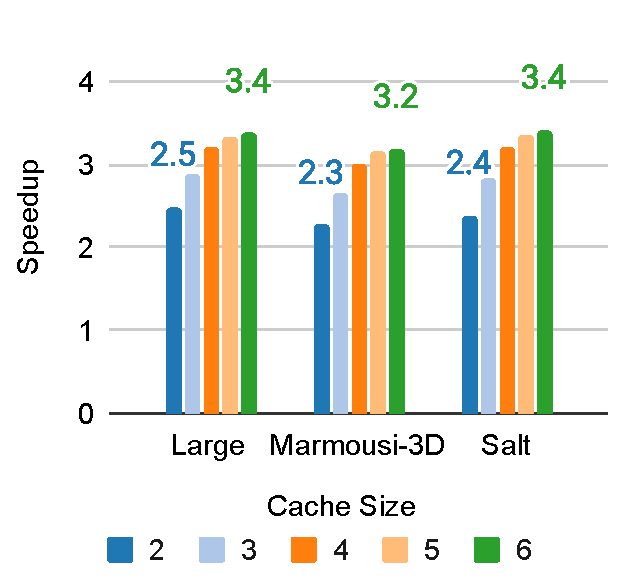
\includegraphics[width=\textwidth]{figures/prefetch_speedup/prefetch_speedup_revolve.pdf}
        \caption{Revolve}
        \label{fig:prefetch_speedup_revolve}
    \end{subfigure}
    \hfill
    \begin{subfigure}[b]{0.33\textwidth}
        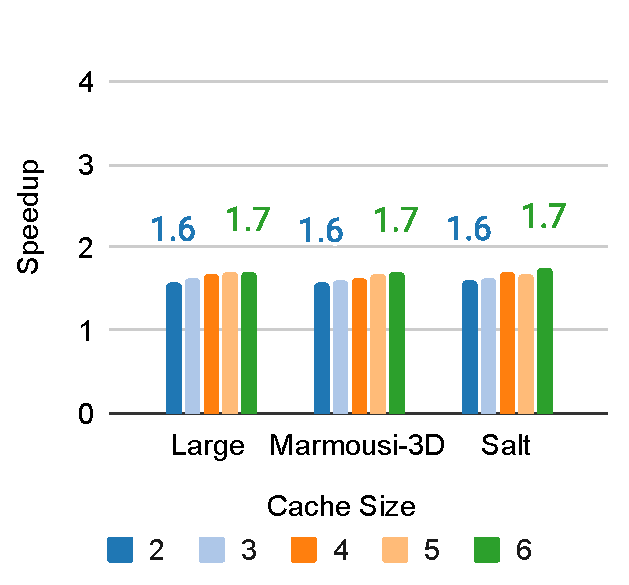
\includegraphics[width=\textwidth]{figures/prefetch_speedup/prefetch_speedup_zcut.pdf}
        \caption{zCut}
        \label{fig:prefetch_speedup_zcut}
    \end{subfigure}
    \hfill
    \begin{subfigure}[b]{0.32\textwidth}
        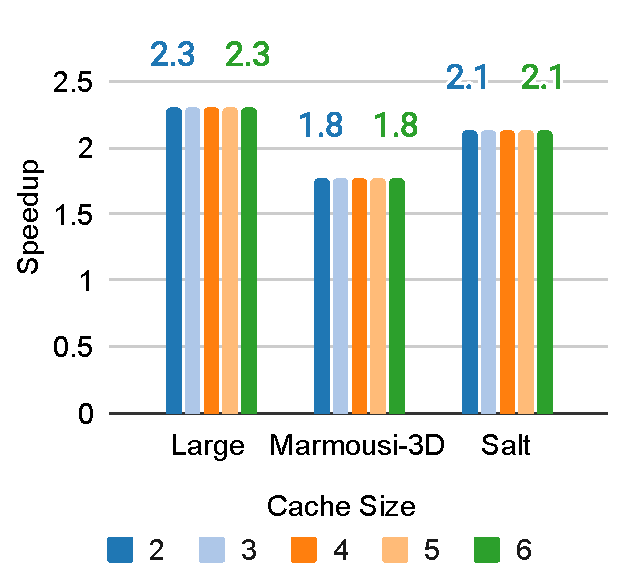
\includegraphics[width=\textwidth]{figures/prefetch_speedup/prefetch_speedup_uniform.pdf}
        \caption{Uniform}
        \label{fig:prefetch_speedup_uniform}
    \end{subfigure}
    
    \caption[Overall speedup (\checkpointprefetching)]{Overall speedup achieved by \revolve (a), \zcut (b), and \uniform (c) for each dataset (Large, Marmousi3D, and Salt). The baseline is the execution of \awave in its base form for the corresponding algorithm and dataset, without caching or prefetching.}
    \label{fig:prefetch_speedup}
\end{figure}

Increasing the cache size influences the prefetching mechanism because with more space to store \checkpointing data, the chances of a checkpoint being in the cache when a \restore occurs are higher (\tit{real hits}). However, the speedup is highly dependent on the \checkpointing algorithm in use.

For example, the \revolve algorithm is the most susceptible to larger cache sizes. Processing a `chunk' (as detailed \rssec{chkpt}) generates up to seven or eight snapshots (depending on the dataset) subsequent \save, which can lead to many cache replacements in a short period. This behavior removes snapshots that will likely be needed soon, as the LRU policy sacrifices the oldest checkpoint to make space for the new one. So, increasing the cache size will help make more snapshots available, causing more \tit{real hits}. The Salt dataset reached $1.8 M$ real cache hits for two cache positions, while the same dataset got $2.2 M$ real cache hits with six cache positions.

In contrast, the \zcut and \uniform algorithms are less sensitive to increases in cache size. \zcut saves about 30 - 40 ``intermediary snapshots'' between major snapshots (depending on the dataset), which can quickly overload the cache. So, increasing the cache size from two to six does not yield significant improvements. This high demand for saving snapshots leads to delays in data transfers between the GPU and CPU while waiting for new entries to be copied.

\uniform captures snapshots only once during the forward phase and does not create additional snapshots afterward. As a result, the time between two successive snapshots can be extensive enough to make the checkpoint available when \restore is requested by the \checkpointing algorithm.

The chart in \rfig{prefetch_breakdown} illustrates how \checkpointprefetching impacts the blocking time spent on communication (orange bars) for \save, summing up the \dth and \dtd copies; and \restore, summing up \htd and \dtd copies. 

The sensitivity to the cache size of \revolve is evident by the reduction in orange bars with larger caches. \zcut also improved blocking transfer time, but bigger cache sizes (3, 4, 5, and 6) do not improve compared to the cache size of 2. \uniform reduced to almost zero the blocking \restore due the long \tit{timeliness}, the remaining orange bar refers to the \dtd time used on restoration.

Another key observation is how asynchronous \save operations benefit from \cache usage. Although \save is nominally asynchronous in the baseline, \awave must wait for the transfer to complete to avoid overwriting data, blocking further computation. With the \cache, \dth transfers are issued asynchronously, but synchronization can still occur if a new snapshot must overwrite a slot still in use. This explains the remaining \save orange bars for \revolve and \zcut.

The overhead may be caused by the prefetching mechanism, and the memory used by the \cache becomes a pertinent concern. The green bars in \rfig{prefetch_breakdown} represent the overhead caused by GPUZIP in the execution time, precisely the time used for memory allocation and the \psa. The green bars demonstrate that the overhead associated with GPUZIP is justified, as it significantly reduces the blocking time for data transfers between GPU and CPU memory. 

\begin{figure*}[]
    \centering
    \begin{subfigure}{0.5\textwidth}
        
\includegraphics[width=\textwidth,trim={0 0 0 0},clip]{figures/prefetch_breakdown/prefetch_breakdown_legend.png}
        \label{fig:prefetch_breakdown_legend}
    \end{subfigure}
    \begin{subfigure}{0.3\textwidth}
        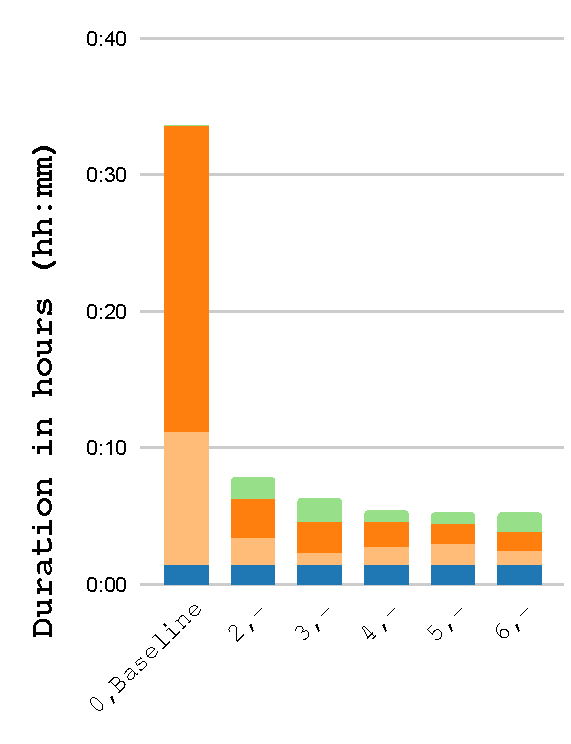
\includegraphics[width=\textwidth,trim={0 0 0 0},clip]{figures/prefetch_breakdown/prefetch_breakdown_revolve_salt.pdf}
        \caption{Revolve}
        \label{fig:prefetch_breakdown_revolve}
    \end{subfigure}%
    \begin{subfigure}{0.3\textwidth}
        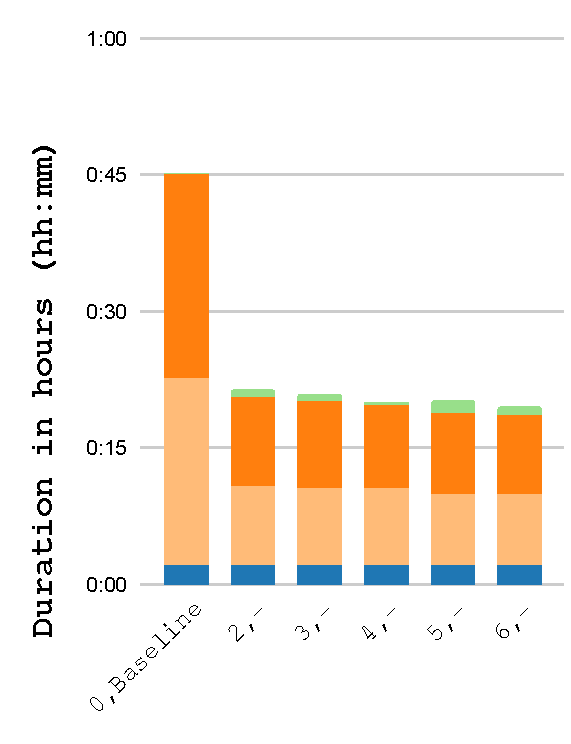
\includegraphics[width=\textwidth,trim={0 0 0 0},clip]{figures/prefetch_breakdown/prefetch_breakdown_zcut_salt.pdf}
        \caption{zCut}
        \label{fig:prefetch_breakdown_zcut}
    \end{subfigure}%
    \begin{subfigure}{0.3\textwidth}
        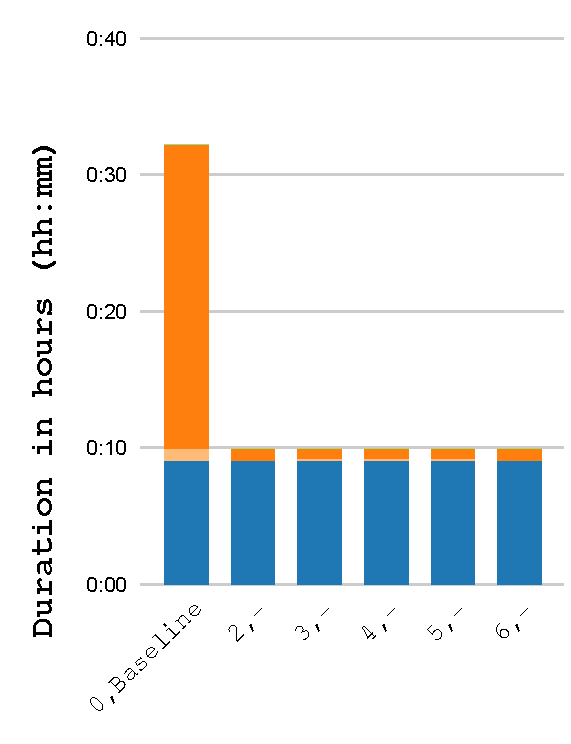
\includegraphics[width=\textwidth,trim={0 0 0 0},clip]{figures/prefetch_breakdown/prefetch_breakdown_uniform_salt.pdf}
        \caption{Uniform}
        \label{fig:prefetch_breakdown_uniform}
    \end{subfigure}\\
    \caption[Execution time breakdown (\checkpointprefetching)]{Execution time breakdown. From cache size 0 (baseline) to 6.}
    \label{fig:prefetch_breakdown}
\end{figure*}

\subsection{Prefetching Mechanism Efficiency}
\label{sec:prefeff}

The prefetching mechanism achieves a $100\%$ cache hit rate across all datasets and algorithms due to the structure of \checkpointing algorithms; since  \restore actions are always interleaved with other computation tasks, there is always an available window to schedule the prefetch before a \restore.

% According to the definition in~\cite{emma2005}, all prefetches in this setup are classified as \tit{good}, since the data was prefetched from host memory into the \cache and was not overwritten by a subsequent \save or \restore operation. 

Nevertheless, \tit{late prefetches} are the hurdle that still causes latencies in the \htd transfers, specially in \revolve and \zcut. The Prefetch action is often issued too close to the checkpoint's rematerialization point, leaving insufficient time to complete the transfer before it is needed. When this occurs, CUDA stream synchronization is required, resulting in stalls. As illustrated in \rfig{prefetch_profile}, a prefetch is dispatched at moment \tinycircled{A1}, initiating an asynchronous transfer. At the moment \tinycircled{A2}, when a \restore is triggered for the in-transit checkpoint, the transfer has not yet completed. Execution must then pause until the data becomes available at \tinycircled{A3}.

The synchronization stalls impact runtime. For instance, with the Marmousi3D dataset and \revolve, synchronization accounts for $4.7\%$ of total execution time with a cache size of 2, and $4.0\%$ with a cache size of 3. For \zcut, the impact is higher $7.8\%$ and $7.6\%$ for cache sizes 2 and 3, respectively. In contrast, \uniform incurs no synchronization overhead, as its design ensures sufficient slack to prefetch all required \checkpointing data.

\begin{figure}[h]
  \centering
  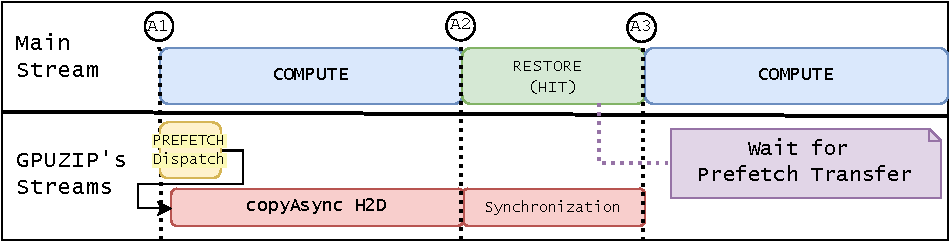
\includegraphics[width=0.7\linewidth,trim={0 0 0 0},clip]{figures/prefetch_profile.pdf}
  \caption[Checkpoint prefetching trace]{Checkpoint prefetching trace. This is a representation of a real NSight trace for prefetching with Marmousi3D and \revolve.}
  \label{fig:prefetch_profile}
\end{figure}

A pertinent concern with the introduced \cache is the required data in the GPU. Users must find a balance between their available GPU memory and the benefits that different cache sizes can bring to their setup. \rtab{prefetch_mem} provides the memory requirements for each \cache for each GPU for various datasets. For example, the smaller fields have lower memory requirements, using about $3.1GB$ per GPU for a cache size of six positions with the Large dataset. In contrast, the M3D\_Larger dataset requires $21GB$ of memory for a cache size of six, which may be unfeasible for some systems or applications.

% GPUZIP enables users to run a few shots for quick checks, allowing them to fine-tune their setup and determine which configuration performs best for the specific problem they are trying to solve.

\begin{table}[h]
\centering
\begin{tabular}{|c|r|r|r|r|}
\hline
\rowcolor[HTML]{C0C0C0} 
\textbf{CacheSize} &
  \multicolumn{1}{c|}{\cellcolor[HTML]{C0C0C0}\textbf{\begin{tabular}[c]{@{}c@{}}Large(GB)\end{tabular}}} &
  \multicolumn{1}{c|}{\cellcolor[HTML]{C0C0C0}\textbf{\begin{tabular}[c]{@{}c@{}}Marmousi3D(GB)\end{tabular}}} &
  \multicolumn{1}{c|}{\cellcolor[HTML]{C0C0C0}\textbf{\begin{tabular}[c]{@{}c@{}}M3D\_Larger(GB)\end{tabular}}} &
  \multicolumn{1}{c|}{\cellcolor[HTML]{C0C0C0}\textbf{\begin{tabular}[c]{@{}c@{}}Salt(GB)\end{tabular}}} \\ \hline
2          & 1.0             & 0.8                 & 7.0                            & 0.9           \\ \hline
3          & 1.6           & 1.2                 & 10.5                         & 1.4           \\ \hline
4          & 2.1           & 1.6                 & 14.0                           & 1.8           \\ \hline
5          & 2.6           & 2.0                   & 17.5                         & 2.3           \\ \hline
6          & 3.1           & 2.4                 & 21.0                           & 2.8           \\ \hline
\end{tabular}

\caption[Memory consumption analysis (\checkpointprefetching)]{GPU Memory required by the \cache on each GPU.}
\label{tab:prefetch_mem}
\end{table}

While the checkpoint prefetching mechanism effectively forecasts cache misses, the synchronization due to \tit{late prefetches} continues to affect overall performance and the data requirements may be high for some scenarios. The prefetch mechanism can benefit from lossy data compression, which will be elaborated in \rch{compress} and integrated with prefetch in \rch{comppref}.

\chapter{Applying Compression on Checkpoint Data}
\label{ch:compress}

Data \compression is commonly used in many fields, including the \compression of files, audio, video, and images~\cite{fz}. It is also crucial for scientific data, which is often large floating-point tensors. This is especially true in applications such as Reverse Time Migration (RTM), climate simulations, and cosmological hydrodynamics simulations~\cite{fz, liu2022, di2025}.

Data \compression not only saves storage space but also reduces the amount of data transferred across different communication channels in computer systems by compressing the data before transmission. For example, it can significantly lower HTTP network traffic~\cite{mogul1997}, reduce CPU and GPU memory traffic~\cite{shen2022,shen2023}, or be applied in multi-layer I/O pipelines, where compressed data is transferred from network storage to a local SSD and then to memory and GPU memory~\cite{maurya2023}.

% The primary bottleneck in \awave lies in the transfer of checkpointing data between the GPU and host memory. During a \save operation, data must be copied from the GPU to the host before the following action can continue, leading to idle GPU time. GPUs are particularly efficient at running compression algorithms~\cite{dmitriev2022}, so GPUs can compress data before sending it to the host, making the transfer to the host memory faster. This strategy aims to reduce the volume of data transferred -- e.g., compressing $100GB$ of data to $50GB$ (a $2\times$ compression ratio) can theoretically cut the transfer time in half. However, the actual speedup depends on whether the time spent compressing and decompressing is smaller than the time saved in data movement, making the balance between compression efficiency and transfer reduction a critical factor.

As discussed in \rchsec{background}{awave3d}, the primary bottleneck in \awave lies in the transfer of \checkpointing data between the GPU and host memory. During a \save operation, the data must be copied from the GPU to the host before the computation can proceed, leading to idle GPU time. One strategy to mitigate this is to compress the data before transferring it, as GPUs are highly efficient at running \compression algorithms~\cite{dmitriev2022}.

Compression improves communication performance when the combined time for compressing, transferring, and decompressing data is less than the time required to transfer the data without \compression. This condition is expressed in~\req{benefit_condition}, based on the total execution time with and without \compression.

The total time when using \compression is given by:

\begin{equation}
T_{\text{total}} = T_{\text{compress}} + T_{\text{transfer\_compressed}} + T_{\text{decompress}}
\label{eq:ttotal}
\end{equation}

\noindent where:
\begin{itemize}
    \item \( T_{\text{compress}} \) is the time to compress the data on the GPU,
    \item \( T_{\text{transfer\_compressed}} \) is the time to transfer the compressed data over PCIe (\dth and \htd),
    \item \( T_{\text{decompress}} \) is the time to decompress the data on the host or GPU.
\end{itemize}

Compression for communication is considered beneficial when the \compression time is lower than the baseline (without \compression):

\begin{equation}
T_{\text{total}} < T_{\text{baseline}}
\label{eq:benefit_condition}
\end{equation}

Beyond cutting the data transfer time, data \compression can reduce the size of the \checkpointing data pool in the host memory. With smaller snapshots, there is more space in the host memory to make more snapshots, in the same direction as Kukreja~\etal~(2020)\cite{kukreja2020}. The \uniform algorithm, for example, can make more snapshots as long as more memory is available.

This chapter is organized as follows: first, \rsec{comp_methodology} presents the methodology used to apply \compression on the checkpoint data, and then \rsec{comp_results} presents the results achieved by using \compression. 


\section{Methodology}
\label{sec:comp_methodology}

This work adopts lossy \compression, a data \compression method that reduces data size by permanently eliminating certain information, particularly in floating-point precision, in contrast to lossless \compression, which preserves all the original data. Lossy \compression results in less data, but the decompressed data will not be identical to the original data. However, the loss can be mitigated by a predefined error-control method, making the data loss insignificant, depending on the intended use of the data~\cite{di2025}. 

This technique has been successfully applied to Reverse Time Migration (RTM) to improve \compression ratios while maintaining high-quality seismic imaging~\cite{kukreja2020, di2025, barbosa2023}, and it is increasingly adopted in other scientific domains as well~\cite{liu2022,di2025}.

This section is organized as follows: \rssec{lossy} provides an overview of the core techniques behind lossy \compression used in this work; next, \rssec{gpubased_lossy} introduces the GPU-based lossy compressors integrated into GPUZIP and highlights their key differences; then, \rssec{eval_qual} presents the metrics used to evaluate these compressors and assess the impact of compression on data quality; and finally, \rssec{comp_awave} explains how the selected compressors were integrated into the \awave through GPUZIP.

\subsection{Lossy Compression}
\label{sec:lossy}

Compressors follow a structured \compression pipeline incorporating multiple techniques, making each compressor unique. The methods used by compressors in this work (Bitcomp, cuZFP, and cuSZp) are: pointwise data prediction (PDP), quantization (QT), bit-plane coding (BPC), discrete cosine transform (DCT), and lossless encoding (LE)\cite{di2025}.

% https://arxiv.org/pdf/2111.09815

\begin{itemize}
    \item \textbf{Pointwise Data Prediction (PDP)} is often the first or second step in modern \compression algorithms. It utilizes a prediction function (e.g., Lorenzo Predictor, linear interpolation, and linear regression) that estimates the value of a data point based on its neighboring/adjacent values (spatial or temporal correlation), then computes the difference between the predicted and original values. This process generates close-to-zero values, which are easier to compress~\cite{di2025,fz,cuszp}.

    \item \textbf{Quantization (QT)} further reduces the data's precision by mapping values to discrete levels, which may be based on either the original values or residuals from the prediction step (PDP)~\cite{di2025,fz}.

    \item \textbf{Lossless encoding (LE)} usually occurs at the end of the \compression process. Its primary purpose is to eliminate redundant values that arise from earlier steps, particularly after quantization (QT), since these values are often very sparse. Huffman Encoding is a well-known example of a lossless encoding algorithm~\cite{di2025}.

    \item \textbf{Discrete Cosine Transform (DCT)} converts spatial data into frequency coefficients, which helps to decorrelate the data, making it more compressible. This transformation results in a few significant coefficients while many others become near zero, allowing these near-zero values to be efficiently encoded using fewer bits. This process enhances compressibility, leading to higher \compression ratios and reduced storage requirements~\cite{di2025}.

    \item \textbf{Bit-Plane Coding (BPC)} is often used after the transform step (e.g., DCT). It encodes data bit by bit, starting with the most significant bits to preserve critical information first. Higher bit planes store the sign, exponent, and the most significant fraction bits for floating-point data. Therefore, truncating lower bit planes reduces precision with minimal impact on the overall data value~\cite{di2025}.
\end{itemize}


Beyond how compressors compress, there is also how they control errors during \compression. The compressors used in this work are categorized based on whether they provide fixed-ratio or error-bounded \compression. 

\textbf{Fixed-ratio} compressors guarantee a specific compression ratio, making them suitable for scenarios with strict memory constraints. The trade-off is in quality, which is sacrificed to reach the desired compression ratio~\cite{di2025}. 

\textbf{Error-bounded} compressors prioritize data fidelity, ensuring that \compression errors remain within a specified limit. These error bounds can be absolute, where the maximum allowable deviation is fixed, or relative, where the error scales proportionally to the data values~\cite{di2025}.

\subsection{GPU-based Lossy Compressors}
\label{sec:gpubased_lossy}

There are multiple known GPU-based lossy compressors~\cite{di2025}, and to choose the compressors to be used in this dissertation, their quality and speed in the related work were evaluated~\cite{dmitriev2022,kukreja2020,shen2022,shen2023,barbosa2023}, and whether they provide APIs to be used by partners. Based on that, the following three libraries were initially chosen:

\begin{itemize}
    \item \textbf{cuSZp}~\cite{cuszp} is one of the latest GPU-based compressors in the SZ family. It utilizes Pointwise Data Prediction (PDP) using a lightweight Lorenzo Predictor, followed by Quantization (QT), which transforms floating-point values into integers using linear-scale quantization. Finally, it employs Lossless Encoding (LE) with a customized Huffman encoder. cuSZp controls its error using an absolute error bound parameter.

    \item \textbf{cuZFP}~\cite{zfp} is a compressor from ZFP family. In contrast to its CPU implementation, the GPU-based implementation only supports fixed-rate mode, which makes the compressed size predictable but does not guarantee quality. The cuZFP \compression scheme begins by dividing the data into small fixed-size blocks. The floating-point values are then converted to a fixed-point representation before applying a transform to decorrelate the data, similar to the DCT explained above, but with some modifications inherited from the ZFP compressor family. Finally, Bit-Plane Coding (BPC) encodes the coefficients. cuZFP expects the parameter \ttt{maxBits}\footnote{\url{https://zfp.readthedocs.io/en/release0.5.4/modes.html\#c.zfp_stream.maxbits} - Accessed May 26, 2025} \footnote{\url{https://zfp.readthedocs.io/en/release0.5.4/modes.html\#mode-fixed-rate} - Accessed May 26, 2025}, which controls the number of bits allocated per value in fixed-rate mode. 

    \item \textbf{NVIDIA's NVCOMP Bitcomp}~\cite{nvcomp}, unlike the open-source compressors used in this study, NVCOMP Bitcomp does not have its source code publicly available. According to the available documentation\footnote{\url{https://docs.nvidia.com/cuda/nvcomp/native_api.html#_CPPv417bitcompCreatePlanP15bitcompHandle_t6size_t17bitcompDataType_t13bitcompMode_t18bitcompAlgorithm_t} - Accessed May 26, 2025}, it is based on the quantization (QT) of floating-point values to integers. The \compression relies on two main parameters: `\ttt{algorithm}', which can be set to either \tit{sparse} or \tit{default}. The \tit{sparse} option performs better with sparse data that contains many zeros\footnote{\url{https://docs.nvidia.com/cuda/nvcomp/cpp_api.html#_CPPv4N6nvcomp23BitcompFormatSpecHeader4algoE} - Accessed May 26, 2025}. The second parameter, `\ttt{delta}', is used for error control, ensuring that errors remain within the specified threshold.
\end{itemize}

\subsection{Evaluating Quality}
\label{sec:eval_qual}

Metrics such as \textbf{PSNR} (\tit{Peak Signal-to-Noise Ratio}) and \textbf{SSIM} (\tit{Structural Similarity Index Measure}) are commonly used to evaluate quantitative quality in studies involving \compression~\cite{cuszp, fz} and also in works addressing \compression for seismic and other scientific fields~\cite{kukreja2020, boehm2016, wang2023}.

\textbf{PSNR} measures the noise introduced by \compression, expressed in decibels (dB). It compares the maximum possible signal power to the noise power on a logarithmic scale, reflecting how humans perceive signal intensity.

The formula for calculating PSNR is:

\begin{equation}
PSNR(f,g) = 10 \times \log_{10}\left(\frac{MAX^2}{MSE(f,g)}\right)
\label{eq:psnr}
\end{equation}

where $f$ represents the baseline image, and $g$ is the comparison image, $MAX$ represents the maximum possible pixel value of the image and $MSE$ is the Mean Square Error that is given by:

\begin{equation}
\text{MSE}(f, g) = \frac{1}{M \times N} \sum_{i=1}^{M} \sum_{j=1}^{N} \left(f_{ij} - g_{ij}\right)^2
\label{eq:mse}
\end{equation}

where $M \times N$ are the image dimentions~\cite{hore2010}.

Although PSNR effectively quantifies distortion, it is less suited for capturing structural differences between images~\cite{hore2010}. To address this limitation, \textbf{SSIM} assesses perceptual similarity, producing values between 0 and 1, where values closer to 1 indicate higher fidelity and structural resemblance. SSIM models image distortion as a combination of luminance, contrast, and structure:

\begin{equation}
\text{SSIM}(f, g) = l(f, g) \cdot c(f, g) \cdot s(f, g)
\label{eq:ssim}
\end{equation}

where $f$ represents the baseline image, and $g$ represents the comparison image~\cite{hore2010}. The components are defined as:

\begin{itemize}
    \item $l(f, g)$ is the luminance comparison function, which evaluates how similar the two images are;
    \item $c(f, g)$ is the contrast comparison function;
    \item $s(f, g)$ is the structure comparison function, which assesses the correlation coefficient between $f$ and $g$.
\end{itemize}



\subsection{Integrating Compression in \awave}
\label{sec:comp_awave}
\rfig{archnew_wcomp} illustrates the \checkpointing workflow in \awave with \compression. When a \save request is made~\circled{1}, the checkpoint data is compressed and stored in a temporary buffer in the GPU. The compressed data is immediately transferred via PCIe to host memory. When a \restore request occurs~\circled{2}, the compressed checkpoint is retrieved from the host memory, transferred to the GPU buffer, and decompressed before rematerialization.

The intermediary GPU buffer is allocated at the start of execution based on the expected \compression ratio. For fixed-rate compressors, this is straightforward: allocate the checkpoint size divided by the known \compression ratio. However, for error-bound \compression, the required buffer size is unknown beforehand. Users can estimate it through experimentation on small executions. For example, using Bitcomp `\ttt{delta=1e-8}' on Marmousi3D, the worst-case \compression ratio is $2.6\times$, defining the buffer size required before running all shots.

The main limitation of using a one-position buffer capable of holding only one compressed checkpoint is its restriction on data access concurrency. For example, if a \save operation is followed closely by a \restore, the \restore must wait for the \save's data transfer to complete before it can proceed. Additionally, all \restore operations are executed synchronously, further reducing potential overlap and performance gains.

% GPUZIP provides a class interface to facilitate experimentation, which each supported compressor implements. The~\rch{oss} details GPUZIP's modular design and API. This approach enables users to test multiple compressors and fine-tune parameters for optimal performance in full-field execution.

\begin{figure}[h]
  \centering
  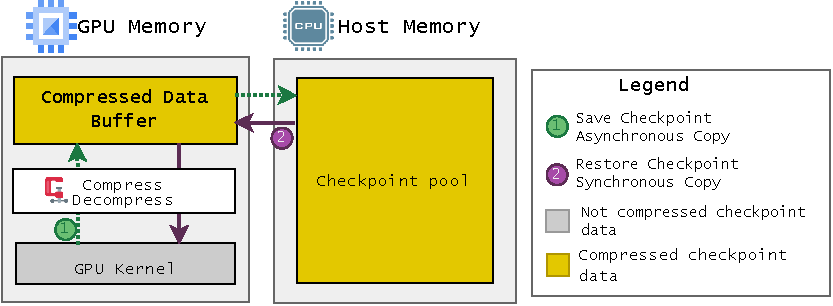
\includegraphics[width=0.9\linewidth,trim={0 0 0 0},clip]{figures/comp_arch.pdf}
  \caption[Memory architecture diagram (\compression)]{GPUZIP's memory architecture with \compression enabled. For every \save, the data is compressed and then saved in a temporary buffer that will be transferred to the host memory. For every \restore, the data will be transferred from the host memory to the temporary GPU buffer and then decompressed and rematerialized.}
  \label{fig:archnew_wcomp}
\end{figure}


\section{Experimental Results}
\label{sec:comp_results}

The effectiveness of \compression in \awave is given by balancing two essential aspects: reducing data movement overhead (speedup) and preserving the quality of the final migrated images --- while higher compression ratios minimize the amount of data transferred through the PCIe interface, they may also introduce quality degradation.

This section is divided into four subsections, each covering a key aspect of the experimental evaluation.~\rsec{compress_exp_setup} describes the experimental setup used to assess the impact of \compression.~\rsec{warmup} presents warm-up experiments with fewer shots to identify optimal compression parameters, balancing compression ratio and output quality. The performance benefits of \compression are detailed in~\rsec{comp_speedup}, highlighting the speedup gains observed when applying \compression to \awave. Finally, ~\rsec{quality} evaluates the quality of the full migrated field produced using the compressed data, analyzing both visual outcomes and quantitative error metrics.

\subsection{Experimental Setup}
\label{sec:compress_exp_setup}

Compression-only experiments were performed across three \checkpointing algorithms (\revolve, \zcut, and \uniform), using the Large, Marmousi3D, and Salt datasets. The same baselines, hardware, compiler versions, and NVIDIA drivers from the prefetching experiments were used (see \rchsec{prefetch}{prefetch_result} for further details).

The optimal \compression parameters for the speedup and quality experiments were determined through initial exploratory tests (described in \rsec{warmup}). These configurations, applied in the performance analysis in \rsec{comp_speedup} and the quality assessment in \rsec{quality}: cuZFP set with $maxBits=8$ and Bitcomp with $delta=1\times10^{-8}$ and default algorithm.

% \begin{itemize}
%     \item \textbf{cuZFP:} \texttt{maxBits} = 8
%     \item \textbf{Bitcomp:} \texttt{delta} = $1 \times 10^{-8}$, \texttt{algorithm} = default
% \end{itemize}

Although this dissertation primarily addresses communication bottlenecks rather than minimizing recomputation, the number of snapshots used during \checkpointing can significantly influence performance. That said, this study does not explore the optimal point at which increasing the number of snapshots yields diminishing returns. \uniform is the only \checkpointing algorithm that attempts to allocate the maximum number of snapshots allowed by the available memory, calculated based on the worst-case compression ratio. In contrast, both \revolve and \zcut use a fixed number of snapshots identical to their respective baselines.

The number of snapshots used in the \uniform setup for each dataset and \compression configuration is as follows in \rtab{uniform_snapshots}.

\begin{table}[h!]
\centering
\begin{tabular}{|l|c|c|c|}
\hline
\rowcolor[HTML]{C0C0C0}
\textbf{Dataset} & \textbf{No Compression} & \textbf{Bitcomp} & \textbf{cuZFP} \\ \hline
Large           & 149                     & 599              & 599            \\ \hline
Marmousi3D      & 177                     & 519              & 674            \\ \hline
Salt            & 149                     & 374              & 535            \\ \hline
\end{tabular}
\caption[Number of snapshots used with \uniform (\compression)]{Number of snapshots used by \uniform under different \compression configs.}
\label{tab:uniform_snapshots}
\end{table}


\subsection{Tuning Compression Parameters}
\label{sec:warmup}

The following experiments were called ``warmup experiments'' because they were conducted with only two shots for each dataset, aiming to calibrate the parameters and determine which compressors would yield the best results for \awave. The experiments utilized the Bitcomp, cuSZp, and cuZFP compressors on the Large, Marmousi3D, and Salt datasets. For Bitcomp, the default algorithm was employed, combining three ``\ttt{delta}'' configurations: \( 1 \times 10^{-2} \), \( 1 \times 10^{-4} \), and \( 1 \times 10^{-8} \). cuSZp was configured to utilize relative errors with \( 1 \times 10^{-2} \), \( 1 \times 10^{-4} \), and \( 1 \times 10^{-8} \) error bounds. In testing cuZFP, `\ttt{maxBits}' configurations of $2$, $4$, and $8$ were assessed.

\rtab{warmup} summarizes the results by reporting the average Compression Ratio (CR), PSNR, and SSIM as quality indicators. To reflect the primary bottleneck of \awave, the table presents the total time spent on data transfers, which is the sum of time used by all four GPUs during execution. Additionally, the table shows the total time spent on compression and decompression, evaluating the overhead introduced by each compressor.

Regarding quality, cuSZp performed poorly. It achieved the worst PSNR and SSIM metrics and had the highest compression and decompression overhead. Its compression ratio ranges from $2.1\times$ to $2.38\times$ for an error bound of \( 1 \times 10^{-8} \).

Bitcomp, on the other hand, performed better for the proposed datasets: considering the `\ttt{delta}' parameter of \( 1 \times 10^{-8} \), it had the highest compression ratios ($115 - 300\times$), the best quality metrics (SSIM very close to $1.00$), and the fastest (de)compression times. 

cuZFP also delivered satisfying quality results, with SSIM close to Bitcomp but more noise (PSNR) than Bitcomp. As a fixed-rate compressor, cuZFP is limited to its predefined ratio of $4\times$ with FP32 on $maxBits=8$.

All compressors can significantly reduce the time spent on (de)compression, including the time involved in communication between the host and the GPU. For instance, when considering the Large dataset in the best-quality scenario for each compressor, the following times were recorded: 2 minutes and 08 seconds for Bitcomp, 06 minutes and 55 seconds for cuSZp, and 04 minutes and 51 seconds for cuZFP. In contrast, the baseline took 37 minutes and 52 seconds. 

The collected data indicates that introducing \compression can alleviate application bottlenecks. On the other hand, quality fidelity is important for this kind of application, so only scenarios that presented SSIM very close to 1 were considered for the all-shots experiments with Awave3D: Bitcomp $delta=1 \times 10^{-8}$ and cuZFP with $maxBits=8$. 

\begin{table}[h!]
\centering
\begin{tabular}{|lrrrrr|}
\hline
\rowcolor[HTML]{C0C0C0} 
\multicolumn{1}{|c|}{\cellcolor[HTML]{C0C0C0}\textbf{Profile}} &
  \multicolumn{1}{c|}{\cellcolor[HTML]{C0C0C0}\textbf{\begin{tabular}[c]{@{}c@{}}CR\\ (AVG)\end{tabular}}} &
  \multicolumn{1}{c|}{\cellcolor[HTML]{C0C0C0}\textbf{PSNR}} &
  \multicolumn{1}{c|}{\cellcolor[HTML]{C0C0C0}\textbf{SSIM}} &
  \multicolumn{1}{c|}{\cellcolor[HTML]{C0C0C0}\textbf{\begin{tabular}[c]{@{}c@{}}Time Spent\\ d2h \& h2d\end{tabular}}} &
  \multicolumn{1}{c|}{\cellcolor[HTML]{C0C0C0}\textbf{\begin{tabular}[c]{@{}c@{}}Time spent\\ (de)comp.\end{tabular}}} \\ \hline
\rowcolor[HTML]{C0C0C0} 
\multicolumn{6}{|l|}{\cellcolor[HTML]{C0C0C0}\textbf{Large}} \\ \hline
\multicolumn{1}{|l|}{baseline} &
  \multicolumn{1}{l|}{-} &
  \multicolumn{1}{l|}{-} &
  \multicolumn{1}{l|}{-} &
  \multicolumn{1}{r|}{0:37:52} &
  \multicolumn{1}{l|}{-} \\ \hline
\multicolumn{1}{|l|}{bitcomp, delta=1e-2} &
  \multicolumn{1}{r|}{678.73} &
  \multicolumn{1}{r|}{44.48} &
  \multicolumn{1}{r|}{0.2481} &
  \multicolumn{1}{r|}{0:00:00} &
  0:00:10 \\ \hline
\multicolumn{1}{|l|}{bitcomp, delta=1e-4} &
  \multicolumn{1}{r|}{228.99} &
  \multicolumn{1}{r|}{67.42} &
  \multicolumn{1}{r|}{0.7952} &
  \multicolumn{1}{r|}{0:00:07} &
  0:00:29 \\ \hline
\multicolumn{1}{|l|}{bitcomp, delta=1e-8} &
  \multicolumn{1}{r|}{137.77} &
  \multicolumn{1}{r|}{140.51} &
  \multicolumn{1}{r|}{1.0000} &
  \multicolumn{1}{r|}{0:02:08} &
  0:00:40 \\ \hline
\multicolumn{1}{|l|}{cuSZp,errBnd=1e-2} &
  \multicolumn{1}{r|}{10.23} &
  \multicolumn{1}{r|}{37.73} &
  \multicolumn{1}{r|}{0.0000} &
  \multicolumn{1}{r|}{0:01:53} &
  0:02:56 \\ \hline
\multicolumn{1}{|l|}{cuSZp,errBnd=1e-4} &
  \multicolumn{1}{r|}{4.66} &
  \multicolumn{1}{r|}{45.61} &
  \multicolumn{1}{r|}{0.0000} &
  \multicolumn{1}{r|}{0:03:29} &
  0:03:46 \\ \hline
\multicolumn{1}{|l|}{cuSZp,errBnd=1e-8} &
  \multicolumn{1}{r|}{2.27} &
  \multicolumn{1}{r|}{45.62} &
  \multicolumn{1}{r|}{0.0000} &
  \multicolumn{1}{r|}{0:06:55} &
  0:05:43 \\ \hline
\multicolumn{1}{|l|}{cuZFP, bitRate=2} &
  \multicolumn{1}{r|}{15.66} &
  \multicolumn{1}{r|}{66.82} &
  \multicolumn{1}{r|}{0.7887} &
  \multicolumn{1}{r|}{0:01:11} &
  0:01:18 \\ \hline
\multicolumn{1}{|l|}{cuZFP, bitRate=4} &
  \multicolumn{1}{r|}{7.83} &
  \multicolumn{1}{r|}{84.51} &
  \multicolumn{1}{r|}{0.9576} &
  \multicolumn{1}{r|}{0:02:24} &
  0:01:32 \\ \hline
\multicolumn{1}{|l|}{cuZFP, bitRate=8} &
  \multicolumn{1}{r|}{3.91} &
  \multicolumn{1}{r|}{111.31} &
  \multicolumn{1}{r|}{0.9995} &
  \multicolumn{1}{r|}{0:04:51} &
  0:01:44 \\ \hline
\rowcolor[HTML]{C0C0C0} 
\multicolumn{6}{|l|}{\cellcolor[HTML]{C0C0C0}\textbf{Marmousi3D}} \\ \hline
\multicolumn{1}{|l|}{baseline} &
  \multicolumn{1}{l|}{-} &
  \multicolumn{1}{l|}{-} &
  \multicolumn{1}{l|}{-} &
  \multicolumn{1}{r|}{1:16:10} &
  \multicolumn{1}{l|}{-} \\ \hline
\multicolumn{1}{|l|}{bitcomp, delta=1e-2} &
  \multicolumn{1}{r|}{597.03} &
  \multicolumn{1}{r|}{41.70} &
  \multicolumn{1}{r|}{0.0057} &
  \multicolumn{1}{r|}{0:00:04} &
  0:01:00 \\ \hline
\multicolumn{1}{|l|}{bitcomp, delta=1e-4} &
  \multicolumn{1}{r|}{205.95} &
  \multicolumn{1}{r|}{65.40} &
  \multicolumn{1}{r|}{0.4589} &
  \multicolumn{1}{r|}{0:00:31} &
  0:01:04 \\ \hline
\multicolumn{1}{|l|}{bitcomp, delta=1e-8} &
  \multicolumn{1}{r|}{115.96} &
  \multicolumn{1}{r|}{95.00} &
  \multicolumn{1}{r|}{1.0000} &
  \multicolumn{1}{r|}{0:06:49} &
  0:01:27 \\ \hline
\multicolumn{1}{|l|}{cuSZp,errBnd=1e-2} &
  \multicolumn{1}{r|}{13.71} &
  \multicolumn{1}{r|}{41.42} &
  \multicolumn{1}{r|}{0.0000} &
  \multicolumn{1}{r|}{0:03:53} &
  0:06:14 \\ \hline
\multicolumn{1}{|l|}{cuSZp,errBnd=1e-4} &
  \multicolumn{1}{r|}{5.42} &
  \multicolumn{1}{r|}{41.51} &
  \multicolumn{1}{r|}{0.0001} &
  \multicolumn{1}{r|}{0:06:41} &
  0:08:03 \\ \hline
\multicolumn{1}{|l|}{cuSZp,errBnd=1e-8} &
  \multicolumn{1}{r|}{2.38} &
  \multicolumn{1}{r|}{41.75} &
  \multicolumn{1}{r|}{0.0001} &
  \multicolumn{1}{r|}{0:15:22} &
  0:12:51 \\ \hline
\multicolumn{1}{|l|}{cuZFP, bitRate=2} &
  \multicolumn{1}{r|}{15.71} &
  \multicolumn{1}{r|}{48.03} &
  \multicolumn{1}{r|}{0.7190} &
  \multicolumn{1}{r|}{0:02:45} &
  0:02:51 \\ \hline
\multicolumn{1}{|l|}{cuZFP, bitRate=4} &
  \multicolumn{1}{r|}{7.85} &
  \multicolumn{1}{r|}{68.72} &
  \multicolumn{1}{r|}{0.9834} &
  \multicolumn{1}{r|}{0:05:33} &
  0:03:32 \\ \hline
\multicolumn{1}{|l|}{cuZFP, bitRate=8} &
  \multicolumn{1}{r|}{3.93} &
  \multicolumn{1}{r|}{98.02} &
  \multicolumn{1}{r|}{0.9996} &
  \multicolumn{1}{r|}{0:11:16} &
  0:04:01 \\ \hline
\rowcolor[HTML]{C0C0C0} 
\multicolumn{6}{|l|}{\cellcolor[HTML]{C0C0C0}\textbf{Salt}} \\ \hline
\multicolumn{1}{|l|}{baseline} &
  \multicolumn{1}{l|}{-} &
  \multicolumn{1}{l|}{-} &
  \multicolumn{1}{l|}{-} &
  \multicolumn{1}{r|}{0:54:10} &
  \multicolumn{1}{l|}{-} \\ \hline
\multicolumn{1}{|l|}{bitcomp, delta=1e-2} &
  \multicolumn{1}{r|}{670.02} &
  \multicolumn{1}{r|}{43.57} &
  \multicolumn{1}{r|}{0.7910} &
  \multicolumn{1}{r|}{0:00:02} &
  0:00:41 \\ \hline
\multicolumn{1}{|l|}{bitcomp, delta=1e-4} &
  \multicolumn{1}{r|}{371.55} &
  \multicolumn{1}{r|}{49.41} &
  \multicolumn{1}{r|}{0.8798} &
  \multicolumn{1}{r|}{0:00:15} &
  0:00:44 \\ \hline
\multicolumn{1}{|l|}{bitcomp, delta=1e-8} &
  \multicolumn{1}{r|}{309.45} &
  \multicolumn{1}{r|}{127.36} &
  \multicolumn{1}{r|}{1.0000} &
  \multicolumn{1}{r|}{0:01:37} &
  0:00:50 \\ \hline
\multicolumn{1}{|l|}{cuSZp,errBnd=1e-2} &
  \multicolumn{1}{r|}{14.86} &
  \multicolumn{1}{r|}{64.61} &
  \multicolumn{1}{r|}{0.0640} &
  \multicolumn{1}{r|}{0:02:32} &
  0:04:00 \\ \hline
\multicolumn{1}{|l|}{cuSZp,errBnd=1e-4} &
  \multicolumn{1}{r|}{4.63} &
  \multicolumn{1}{r|}{45.51} &
  \multicolumn{1}{r|}{0.0641} &
  \multicolumn{1}{r|}{0:05:28} &
  0:05:32 \\ \hline
\multicolumn{1}{|l|}{cuSZp,errBnd=1e-8} &
  \multicolumn{1}{r|}{2.12} &
  \multicolumn{1}{r|}{46.87} &
  \multicolumn{1}{r|}{0.0640} &
  \multicolumn{1}{r|}{0:12:52} &
  0:08:53 \\ \hline
\multicolumn{1}{|l|}{cuZFP, bitRate=2} &
  \multicolumn{1}{r|}{15.77} &
  \multicolumn{1}{r|}{43.76} &
  \multicolumn{1}{r|}{0.8464} &
  \multicolumn{1}{r|}{0:01:45} &
  0:01:26 \\ \hline
\multicolumn{1}{|l|}{cuZFP, bitRate=4} &
  \multicolumn{1}{r|}{7.89} &
  \multicolumn{1}{r|}{62.52} &
  \multicolumn{1}{r|}{0.9182} &
  \multicolumn{1}{r|}{0:03:32} &
  0:01:36 \\ \hline
\multicolumn{1}{|l|}{cuZFP, bitRate=8} &
  \multicolumn{1}{r|}{3.94} &
  \multicolumn{1}{r|}{87.18} &
  \multicolumn{1}{r|}{0.9919} &
  \multicolumn{1}{r|}{0:07:10} &
  0:01:45 \\ \hline
\end{tabular}
\caption[Compression warm-up experiments results]{Compression warm-up experiment results using \awave on two shots. The columns are defined as follows: \textbf{CR (AVG)}: Average Compression Ratio (higher is better); \textbf{PSNR}: higher is better; \textbf{SSIM}: values closer to $1$ indicate more similarity to the baseline; \textbf{Time Spent d2h \& h2d}: Total time (h:m:s) for four GPUs during \dth (d2h) and \htd (h2d) communication; \textbf{Comp. \& Decomp.}: Total time (h:m:s) for compression and decompression across the same four GPUs.}
\label{tab:warmup}
\end{table}


\subsection{Overall Speedup}
\label{sec:comp_speedup}

Applying \compression in \awave provided substantial speedups across all \checkpointing libraries, datasets, and compressors evaluated as displayed in \rfig{compress_speedup}.

\begin{figure*}[h!]
    \centering

    % Row 1: Revolve
    \begin{subfigure}[b]{0.33\textwidth}
        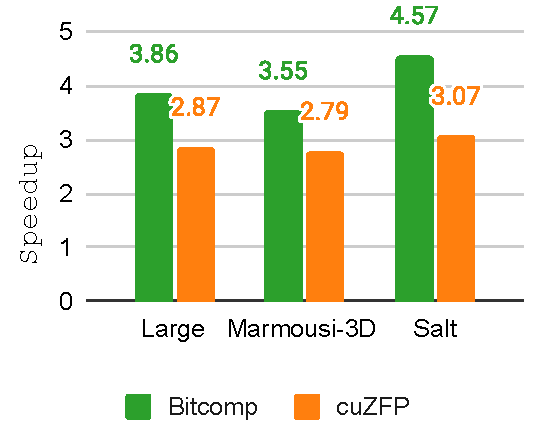
\includegraphics[width=\textwidth]{figures/compress_speedup/speedup_compress_revolve.pdf}
        \caption{Revolve}
        \label{fig:compress_speedup_revolve}
    \end{subfigure}
    \hfill
    \begin{subfigure}[b]{0.33\textwidth}
        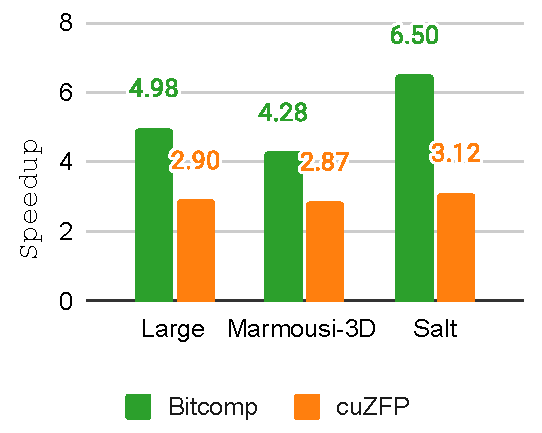
\includegraphics[width=\textwidth]{figures/compress_speedup/speedup_compress_zcut.pdf}
        \caption{zCut}
        \label{fig:compress_speedup_zcut}
    \end{subfigure}
    \hfill
    \begin{subfigure}[b]{0.32\textwidth}
        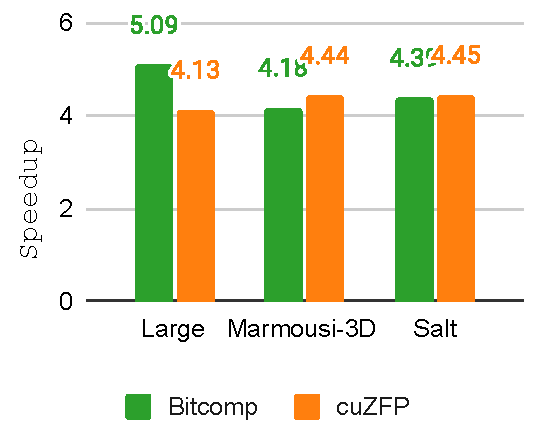
\includegraphics[width=\textwidth]{figures/compress_speedup/speedup_compress_uniform.pdf}
        \caption{Uniform}
        \label{fig:compress_speedup_uniform}
    \end{subfigure}
    
    \caption[Overall speedup (\compression)]{Overall speedup achieved by applying Bitcomp and cuZFP compressors across three datasets (Large, Marmousi3D, and Salt). Each subfigure presents results for a specific \checkpointing algorithm. Baselines consider no \compression, saving checkpoint data directly to the host memory, and restoring from the host memory to be rematerialized in the GPU memory.}
    
    \label{fig:compress_speedup}
\end{figure*}

Starting with \revolve (\rfig{compress_speedup_revolve}), it is possible to observe that Bitcomp consistently achieves higher speedups, ranging from $3.55\times$ to $4.57\times$ across datasets. cuZFP also delivers noticeable improvements, with speedups between $2.79\times$ and $3.07\times$. The source of these gains comes from the reduction in communication overhead. This behavior is clearly illustrated in \rfig{compress_breakdown_revolve}, where the computation time (blue bars) remains stable across all setups (baseline, Bitcomp, and cuZFP), while the communication time (orange bars, representing device-to-host and host-to-device transfers) significantly decreases when \compression is applied. In contrast, the overhead of compression and decompression operations is almost negligible compared to the overall execution time.

Moving to \zcut (\rfig{compress_speedup_zcut}), the benefits of using \compression become even more pronounced. Bitcomp achieves speedups as high as $6.5\times$ for the Salt dataset, while cuZFP maintains improvements between $2.87\times$ and $3.12\times$. Again, the main driver of these gains is the reduction in communication cost, as shown in \rfig{compress_breakdown_zcut}, following the same pattern observed in Revolve. 

%\uniform behaves differently from other \checkpointing strategies. While Bitcomp still delivers strong speedups, cuZFP slightly outperforms it for the Marmousi3D and Salt datasets. Notably, cuZFP's advantage does not stem from reduced communication time but rather from a greater reduction in recomputation. \uniform can dynamically adapt to the available memory budget and allocate as many snapshots as possible.

% \uniform behaves differently from other \checkpointing strategies. While Bitcomp still delivers strong speedups, cuZFP slightly outperforms it for the Marmousi3D and Salt datasets. \uniform can dynamically adapt to the available memory budget and allocate as many snapshots as possible.

 \uniform can dynamically adapt to the available memory budget and allocate as many snapshots as possible. Thanks to cuZFP's predictable and stable compression ratio of $4\times$ (considering 32-bit floating-point data and \ttt{maxBits} = 8) \uniform can consistently store more snapshots, minimizing redundant computations. In contrast, Bitcomp's compression ratio varies between $2.0\times$ and $2.6\times$, based on the worst-case values observed during the warmup experiments (as seen in \rtab{warmup}). So cuZFP slightly outperforms Bitcomp for the Marmousi3D and Salt dataset for \uniform cases, since with cuZFP \uniform could take more snapshots and avoid more recomputation.

An exception appears in the Large dataset. Due to its sparse nature, its worst-case compression ratio with Bitcomp is higher than other datasets and achieves the same number of snapshots as cuZFP. In this scenario, Bitcomp provides a greater overall speedup because it can reduce communication more effectively than cuZFP, as observed in \revolve and \zcut experimentation.

It is important to highlight that the speedup observed for \uniform is primarily influenced by its ability to increase the number of snapshots due to \compression. For instance, in the baseline execution of the Marmousi3D dataset, only 177 snapshots were used. When using Bitcomp, this number increased to 519, and with cuZFP, to 674. If the compressed versions had been restricted to the same 177 snapshots as the baseline, the speedups would have dropped significantly, from $4.18\times$ to $1.88\times$ for Bitcomp, and from $4.44\times$ to $1.79\times$ for cuZFP. This underscores that beyond \compression reduces data transfer overhead, it also enables the storage of more snapshots, thereby decreasing recomputation costs; an advantage also highlighted in previous studies such as \cite{kukreja2020}.

The \uniform behavior described is further illustrated in \rfig{compress_breakdown_uniform}, showing that \compression in \uniform helped reduce computation and communication time. Unlike other \checkpointing schemes, \uniform performs its \save operations only at the beginning of the execution, and does not take more intermediate data after the backward phase starts.

A common trend observed in all checkpoint algorithms executions in \rfig{compress_breakdown}: decompression times are longer than compression times. This discrepancy is not due to decompression being inherently slower; rather, it is because \restore operations, which necessitate decompression, occur much more often than \save operations, which involve compression. In general, decompression operations are faster than compression.

Overall, these results demonstrate the effectiveness of compressors in reducing communication bottlenecks and accelerating \awave while introducing minimal overhead from compression and decompression tasks, satisfying in all scenarios the \req{benefit_condition}.

\begin{figure*}[h!]
    \centering
    \begin{subfigure}{0.8\textwidth}
        
\includegraphics[width=\textwidth,trim={0 0 0 0},clip]{figures/compress_breakdown/legend.png}
        \label{fig:compress_breakdown_legend}
    \end{subfigure}
    \begin{subfigure}{0.3\textwidth}
        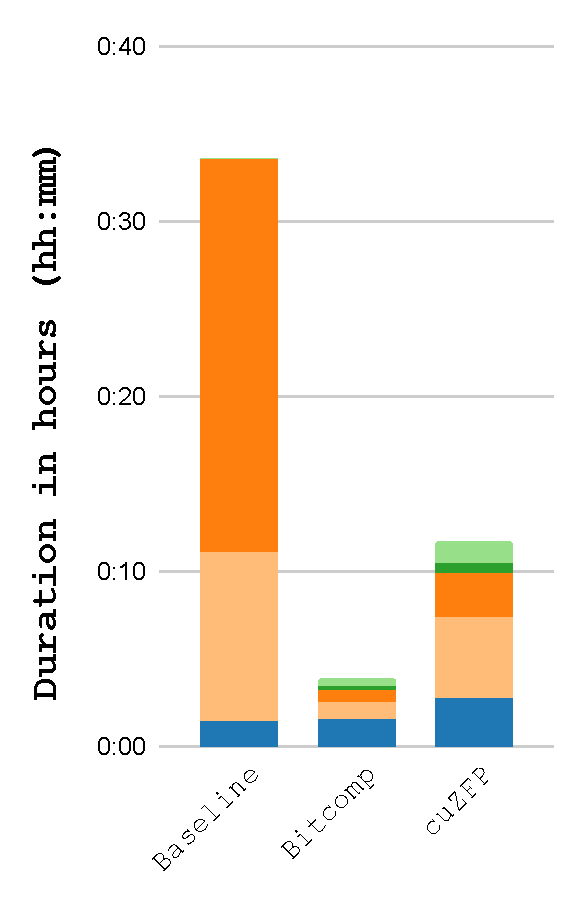
\includegraphics[width=\textwidth,trim={0 0 0 0},clip]{figures/compress_breakdown/breakdown_compress_salt_revolve.pdf}
        \caption{Revolve}
        \label{fig:compress_breakdown_revolve}
    \end{subfigure}%
    \begin{subfigure}{0.3\textwidth}
        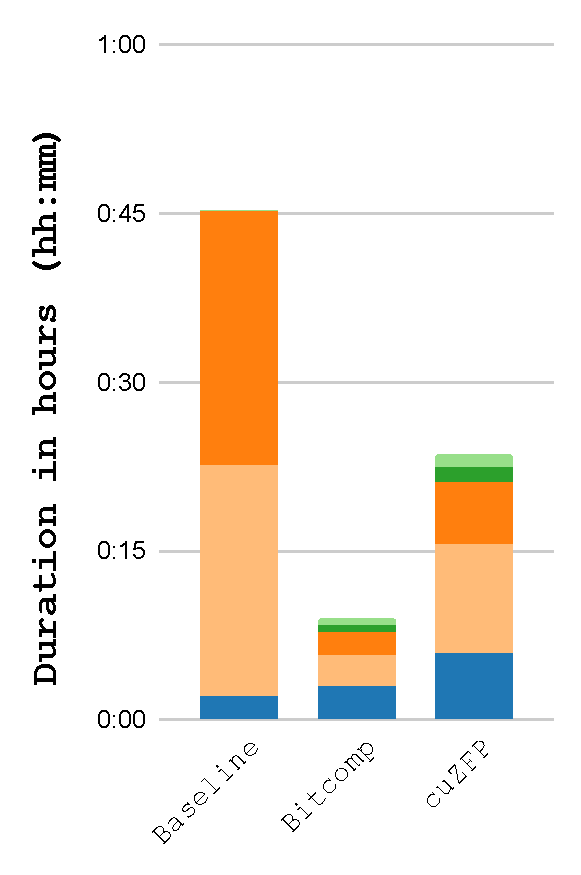
\includegraphics[width=\textwidth,trim={0 0 0 0},clip]{figures/compress_breakdown/breakdown_compress_salt_zcut.pdf}
        \caption{zCut}
        \label{fig:compress_breakdown_zcut}
    \end{subfigure}%
    \begin{subfigure}{0.3\textwidth}
        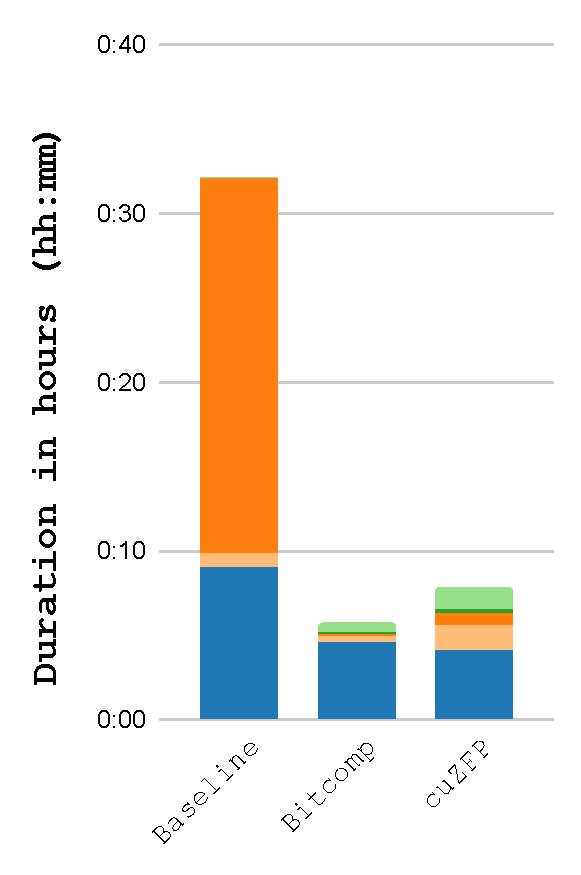
\includegraphics[width=\textwidth,trim={0 0 0 0},clip]{figures/compress_breakdown/breakdown_compress_salt_uniform.pdf}
        \caption{Uniform}
        \label{fig:compress_breakdown_uniform}
    \end{subfigure}\\
    \caption[Execution time breakdown (\compression)]{Execution time breakdown for Salt dataset.}
    \label{fig:compress_breakdown}
\end{figure*}

\subsection{Quality Assessment}
\label{sec:quality}

A qualitative assessment was performed to evaluate whether \compression would visually impact the final migrated images generated by \awave. 

Identifying perceptible differences between the migrated images using \compression and the baseline without \compression is challenging after visually inspecting the resulting images. In \rfig{render_baseline_salt}, a frame from the Salt dataset is shown without \compression, along with the compressed versions, Bitcomp (\rfig{render_bitcomp_salt}) and cuZFP (\rfig{render_cuzfp_salt}). \rfig{errmap_salt} presents an absolute error map that reveals some minor discrepancies in shades of red. Additionally, it is essential to note that the highest error in this dataset is 0.08 within the -750 to 750 interval, indicating that the images produced by the baseline and GPUZIP appear identical to the naked eye. The overall 3D field and other datasets demonstrate similar results, which can be examined and viewed in the reproducibility data available in \cite{ds}.

For the quantitative analysis, \rtab{quality} summarizes the results of the PSNR (Peak Signal-to-Noise Ratio) and SSIM (Structural Similarity Index) metrics across the three datasets used in this study. Regarding PSNR, Bitcomp consistently achieves higher values than cuZFP across all datasets. However, the SSIM values for both compressors are very close to $1.00$ across all datasets, suggesting that, from a structural similarity perspective, the compressed images retain excellent fidelity to the original images.

The quantitative result aligns with the qualitative analysis and supports the conclusion that GPUZIP \compression preserves the integrity of the final seismic images, even with aggressive data reduction strategies.



\begin{table}[h!]
\centering
\begin{tabular}{|l|l|l|l|}
\hline
\rowcolor[HTML]{C0C0C0}
\textbf{Dataset} & \textbf{Compressor} & \textbf{PSNR} & \textbf{SSIM} \\ \hline
\textbf{Large}   & cuZFP      & 105.98  & 0.99  \\ \cline{2-4} 
                 & Bitcomp    & 138.06  & 0.99  \\ \hline
\textbf{Marmousi3D} & cuZFP   & 94.23   & 0.99  \\ \cline{2-4} 
                    & Bitcomp & 120.94  & 0.99  \\ \hline
\textbf{Salt}    & cuZFP      & 78.01   & 0.99  \\ \cline{2-4} 
                 & Bitcomp    & 135.82  & 0.99  \\ \hline
\end{tabular}
\caption[Compression quality assessment]{Comparison of PSNR and SSIM for cuZFP and Bitcomp across all datasets. Higher PSNR and SSIM values indicate better quality and greater similarity to the baseline image.}
\label{tab:quality}
\end{table}


\begin{figure*}[]
    \centering
    \begin{subfigure}{0.49\textwidth}
        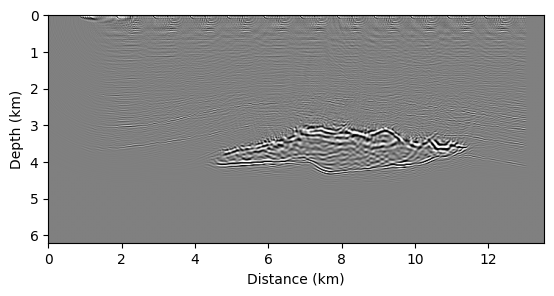
\includegraphics[width=\textwidth,trim={4px 0 0 0}, clip]{figures/quality/render_baseline_salt.png}
        \caption{Baseline}
        \label{fig:render_baseline_salt}
    \end{subfigure}
    \hfill
    \begin{subfigure}{0.49\textwidth}
        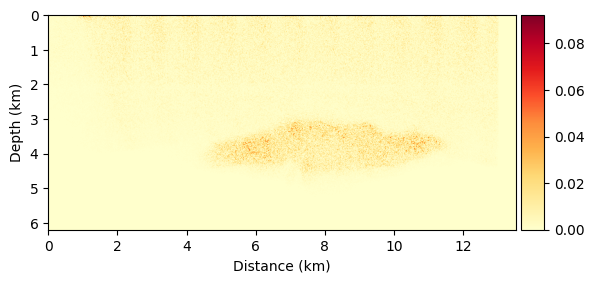
\includegraphics[width=\textwidth,trim={35px 0 8px 0px}, clip]{figures/quality/errormap_bitcomp_salt.png}
        \caption{Error Map with Bitcomp}
        \label{fig:errmap_salt}
    \end{subfigure}
    \hfill
    \begin{subfigure}{0.49\textwidth}
        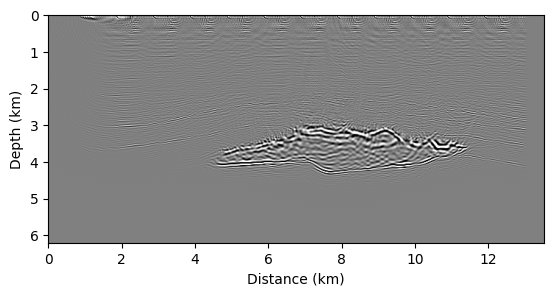
\includegraphics[width=\textwidth,trim={4px 0 0 0}, clip]{figures/quality/render_cuzfp_salt.png}
        \caption{cuZFP}
        \label{fig:render_cuzfp_salt}
    \end{subfigure}
    \hfill
    \begin{subfigure}{0.49\textwidth}
        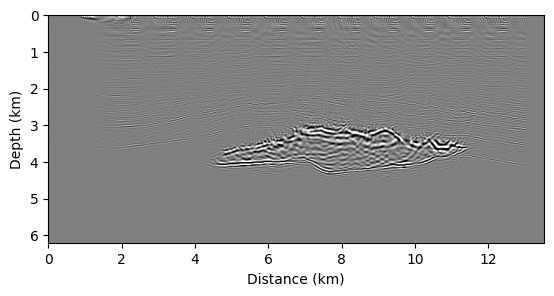
\includegraphics[width=\textwidth,trim={4px 0 0 0}, clip]{figures/quality/render_bitcomp_salt.png}
        \caption{Bitcomp}
        \label{fig:render_bitcomp_salt}%
    \end{subfigure}
    \hfill
    \caption[Comparison of migrated images for Salt dataset]{Comparison of migrated images for Salt dataset}
    \label{fig:quality}
\end{figure*}




\chapter{Combining Compression and Prefetching}
\label{ch:comppref}

The \checkpointprefetching mechanism benefits \awave, with speedups up to $3.4\times$ with \revolve, $1.7\times$ with \zcut, and $2.3\times$ with \uniform. These gains are primarily due to reducing blocking time on the PCIe bus by retrieving checkpoint data in advance and reusing data already stored in the cache.

Applying \checkpointing data \compression is also worthwhile to \awave. Depending on the dataset, it can increase speedups to $4.57\times$ with \revolve, $6.5\times$ with \zcut, and $5.09\times$ with \uniform. These improvements stem from reducing the amount of data transferred over PCIe, thus alleviating one of \awave's main performance bottlenecks.

Both techniques can be combined: \compression can help prefetch be faster if the checkpoint data to be prefetched were smaller, so it can be transferred faster, meeting with the prefetching \tit{timeliness}.

This chapter is organized as follows: \rsec{comppref_methodology} presents the decisions made regarding combining both techniques, and \rsec{comppref_results} presents the experimental results of the methodology adopted.

\section{Methodology}
\label{sec:comppref_methodology}

The main hurdle for prefetching is that the prefetched checkpoint does not have enough time to come from the host memory to the GPU memory before the checkpoint algorithm performs a \restore action; this makes the GPU idle while the checkpoint data synchronization happens.

The timeline \circled{A} in \rfig{async} illustrates the concurrency scenario: the \tit{Prefetch Dispatch} \tinycircled{A1} asynchronously transfers a checkpoint of $400MB$ from the host to the GPU. At the same time, the computation of a kernel (``\ttt{COMPUTE}'' that is a sequence of \fwd and \bwd) is happening. However, when the \restore in \tinycircled{A2} occurs, the checkpoint requested is still being transferred. Hence, the GPU is idle waiting for the synchronization to finish, and then ``\ttt{COMPUTE}'' can forward in \tinycircled{A3}.

\begin{figure}
  \centering
  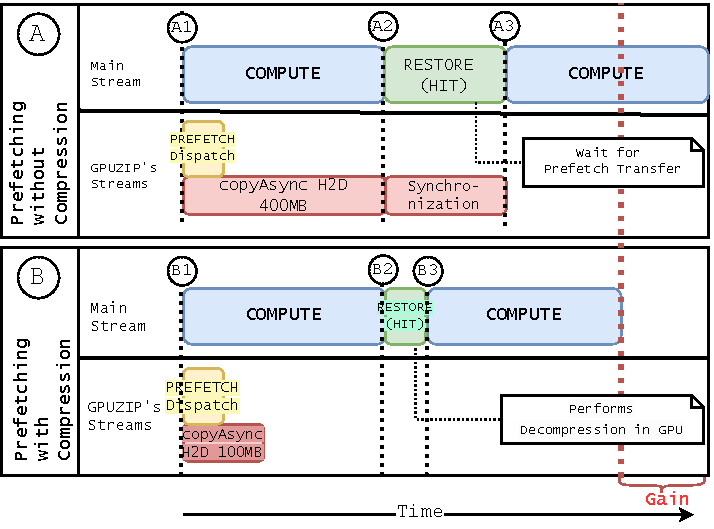
\includegraphics[width=0.8\linewidth,trim={0 0 0 0},clip]{figures/async.pdf}
  \caption[Timeliness for \checkpointprefetching with and without \compression]{Timelines showing prefetching traces: Timeline "A" depicts no \compression applied to checkpoint data, while Timeline "B" illustrates the effects of \compression on prefetching data. The dotted red line highlights the efficiency gain from \compression.}
  \label{fig:async}
\end{figure}

In contrast, Timeline \circled{B} illustrates how \compression effectively addresses the bottleneck observed in \circled{A}. During the \tit{Prefetch Dispatch} phase \tinycircled{B1}, a $4\times$ compressed checkpoint is transferred, significantly reducing \htd data movement. Consequently, when the \restore operation \tinycircled{B2} is triggered, the checkpoint data is already present in the GPU memory, allowing for immediate decompression and seamless resumption of execution \tinycircled{B3}. The interval marked as ``\ttt{Gain}'' reflects the resulting performance benefit from this optimization.

\ralg{gpuzip_loop} outlines the execution loop for integrating prefetching and \compression in \awave. Initially, the \tit{Prefetch Setup} occurs with the configured cache size (line 1). At this stage, the user can decide to increase the cache size, as compressed data will be smaller than uncompressed data, e.g., if it is known that the compressed data is $2\times$ smaller, the cache size can be doubled compared to a situation without \compression and then store more snapshots in the \cache. Another scenario where \compression can be beneficial is when dealing with a large data field that could not accommodate a minimum cache size of two positions; with \compression, the smaller data could now fit into the available space.

Still following~\ralg{gpuzip_loop}, line 3 will determine the following \checkpointing action. If prefetching conditions are met, a dispatch is triggered to load future checkpointing data in advance (lines 4–6). When a \save action occurs, the computing data is compressed directly into the \cache. Compressors will perform a \dtd (D2D) copy behind the scenes, and then the \cache will transfer the compressed data to the host memory (D2H) (lines 7–9). 

If a \restore action is issued, the system checks whether the required timestep is already in the cache (line 11). If it is and the transfer is still ongoing, it waits for completion (lines 12–14), then it will decompress the data directly to the computation data (D2D) (line 15). Otherwise, the worst scenario, the cache miss, will happen: it transfers the compressed checkpoint from host to cache (H2D) and decompresses it for computation (D2D) (lines 16–19).

The latest version of GPUZIP is the result of combining \compression and \prefetching techniques. \rfig{arch_gpuzip} presents the GPUZIP architecture, which extends the prefetching architecture, preserving the \cache and \pool structure along with its stream and policy mechanisms.

On \save operations, the checkpoint data is compressed and compressor dumps data directly to the \cache \circled{1}, then GPUZIP explicitly copies the compressed data from the \cache to the \pool (\dth). On \restore \circled{2} or prefetch \circled{3}, the data moves in the opposite direction, the compressed data is copied from the \pool to the \cache (\htd), and before re-materialization, the data is decompressed. Compressor dumps the data directly to the \awave reserved memory to go forward with the computation.

\begin{algorithm}
\caption{Checkpointing Prefetching with Compression Execution Loop}
\label{alg:gpuzip_loop}
\begin{algorithmic}[1]
\STATE $pav \gets$ PrefetchSetup($config.cacheSize$)

\WHILE{action $\neq$ TERMINATE}
    \STATE action $\gets$ Checkpointing.GetAction()
    \IF{pav.shouldDispatch()}
        \STATE pav.dispatch()
    \ENDIF
    
    \IF{action == SAVE}
        \STATE Compress computing data directly to the cache (D2D)
        \STATE Save from cache to host (D2H)
    \ELSIF{action == RETRIEVE}
        \IF{currentTimestep is in cache}
            \IF{transfer is still happening} 
                \STATE Wait for the transfer to finish
            \ENDIF
            \STATE Decompress from Cache directly to computing data (D2D) \COMMENT{Cache Hit!}
        \ELSE
            \STATE Copy from host to cache (H2D)
            \STATE Decompress from Cache directly to computing data (D2D)
        \ENDIF
    \ELSIF{action == FORWARD or action == BACKWARD}
        \STATE Perform forward or backward computation
    \ENDIF
\ENDWHILE
\end{algorithmic}
\end{algorithm}


\begin{figure}[]
  \centering
  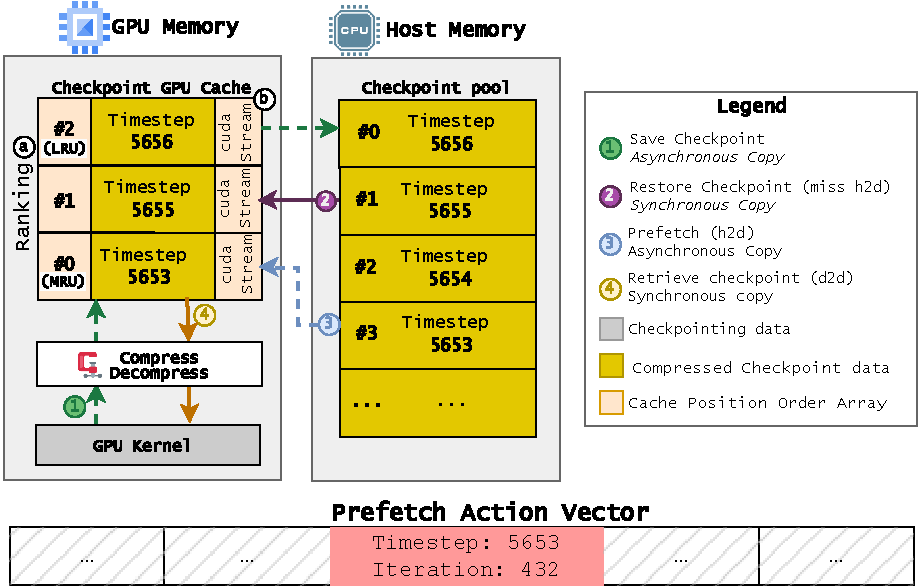
\includegraphics[width=0.95\linewidth,trim={0 0 0 0},clip]{figures/arch_gpuzip.pdf}
  \caption[Memory architecture diagram (\checkpointprefetching + \compression)]{GPUZIP's memory architecture}
  \label{fig:arch_gpuzip}
\end{figure}

\section{Experimental Results}
\label{sec:comppref_results}

This section presents the experimental evaluation of combining GPUZIP’s prefetching mechanism with data compression. The goal is not only to assess the effectiveness of this integration but also to compare it with previously evaluated techniques -- prefetching-only (\rch{prefetch}) and \compression-only (\rch{compress}) -- to identify the most effective configurations for each \checkpointing algorithm and dataset.

This section is organized as follows:
\begin{itemize}
    \item \rsec{comppref_experimental_setup} details the experimental setup and profiles evaluated.
    \item \rsec{comppref_speeudup} presents the speedups achieved by combining \prefetching and \compression.
    \item \rsec{comppref_mem} analyzes memory usage under different configurations.
    \item \rsec{comppref_scalability} evaluates scalability across multiple nodes.
\end{itemize}

\subsection{Experimental Setup}
\label{sec:comppref_experimental_setup}

The experiments use the same three \checkpointing algorithms—\revolve, \zcut, and \uniform—and the same datasets: Large, Marmousi3D, and Salt. Hardware and software environments are identical to those described in \rchsec{prefetch}{prefetch_result}, and the \compression parameters follow those used in \rchsec{compress}{compress_exp_setup}.

Each \checkpointing algorithm is evaluated using its standard implementation in \awave as the baseline. In this default setup, all checkpoint data is stored in host memory and synchronously transferred to the GPU during restore operations. These baselines do not use caching, \compression, or \prefetching.

The \compression configurations are:

\begin{itemize}
    \item \textbf{Bitcomp}: \texttt{delta} = $1 \times 10^{-8}$, \texttt{algorithm} = default
    \item \textbf{cuZFP}: \texttt{maxBits} = 8
\end{itemize}

The cache sizes evaluated range from 2 to 6, consistent with the configurations from \rch{prefetch}. Cache sizes that produced identical results are not shown to maintain clarity and avoid redundancy in the result tables. Complete experimental data, including all cache sizes, is available in the reproducibility repository~\cite{ds}.

The evaluated profiles are:

\begin{itemize}
    \item \textbf{Prefetching} – GPUZIP prefetching without \compression.
    \item \textbf{cuZFP} – Compression-only using cuZFP.
    \item \textbf{Bitcomp} – Compression-only using NVIDIA’s Bitcomp.
    \item \textbf{Prefetching + cuZFP} – Combination of prefetching and cuZFP.
    \item \textbf{Prefetching + Bitcomp} – Combination of prefetching and Bitcomp.
\end{itemize}

\subsection{Overall Speedup}
\label{sec:comppref_speeudup}
To evaluate the combined impact of prefetching and \compression, \rtabn{gpuzip_revolve_speedup}{gpuzip_zcut_speedup}{gpuzip_uniform_speedup} present the speedups achieved using each technique individually and then combined, with both compressors (cuZFP and Bitcomp).

Starting with \revolve (\rtab{gpuzip_revolve_speedup}), prefetching increases speedups as the cache grows. Compression alone yields even greater gains, though this depends on how compressible the data is. The best performance results from combining both techniques. With cuZFP, speedups range from $4.1\times$ to $4.6\times$ at cache size 4; cache sizes 5 and 6 are omitted due to saturation. Bitcomp reaches its saturation point at cache size 4, since the smaller data size (due to \compression) allows prefetching to occur in time before \restore.

As shown in \rfig{breakdown_revolve}, this combined approach nearly eliminates the blocking time (orange bars) caused by \dth and \htd transfers. The GPUZIP overhead (green bars) -- which includes compression, decompression, and internal method calls like \psa -- remains minimal. Prefetching-only configurations still show the \save operation as a bottleneck due to synchronization delays when a new snapshot must wait for the previous one to finish transferring. Compression alleviates this by making \dth faster, reducing \save blocking almost entirely.

Speedups for \zcut (\rtab{gpuzip_zcut_speedup}) are less sensitive to cache size, regardless of whether \compression is applied. Compression alone already brings notable improvements, but combining it with prefetching further enhances performance, up to $8.8\times$ with Bitcomp at cache size 2. The limited reactivity to cache size stems from \zcut's tendency to save many intermediate snapshots, quickly saturating the cache. Here, \compression is crucial to reduce \save overhead. Still, the prefetching mechanism helps by preparing data for \restore ahead of time. \rfig{breakdown_zcut} confirms these observations: blocking times drop, and GPUZIP overhead remains negligible.

For \uniform (\rtab{gpuzip_uniform_speedup}), \compression has a strong impact by allowing more checkpointing data to be stored. Prefetching, on the other hand, significantly reduces \htd delays. Combining both techniques delivers the best results: Bitcomp performs better on the Large dataset, while cuZFP leads on Marmousi and Salt. This difference is attributed to cuZFP's higher fixed \compression ratio ($4\times$), which enables more snapshots than Bitcomp ($2.6\times$ worst case). Thus, \uniform benefits from three factors: (a) increased snapshots, (b) smaller transfer volume, and (c) hidden transfer latency through prefetching.

As shown in \rfig{breakdown_uniform}, restore operations are the main bottleneck in \uniform's baseline. Combining \compression and prefetching reduces this time to nearly zero. Worth noting that the remaining \dtd copies presented in prefetching-only experimentation are hidden with \compression because the compressor dumps the snapshot directly to the cache, so now, that \dtd copy is hidden in the green bars.

An important point arises from \uniform: if restoration points are already far apart, why does not prefetching alone yield the same gains as the combination? The key is the checkpoint quantity. Compression enables storing more snapshots, reducing recomputation, and speeding up the overall execution. Without increasing the number of snapshots, \compression brings no advantage over prefetching alone; speedups drop to $1.84\times$ (Bitcomp) and $1.81\times$ (cuZFP) on Marmousi3D. In short, \compression helps not through faster transfers (as in other \checkpointing algorithms) but by enabling more frequent snapshots.

In summary, across all configurations, \rfig{breakdown} shows that GPUZIP's internal overhead (green bars) is consistently low. This small cost is far outweighed by the reduction in communication time (orange bars), which remains the primary bottleneck addressed by GPUZIP.

\begin{table}[h!]
\centering
\begin{tabular}{|l|rrrrr|rr|rrrr|rrr|}
\hline
\rowcolor[HTML]{C0C0C0} 
\multicolumn{1}{|c|}{\cellcolor[HTML]{C0C0C0}} &
  \multicolumn{5}{c|}{\cellcolor[HTML]{C0C0C0}\textbf{Prefetch Only}} &
  \multicolumn{2}{c|}{\cellcolor[HTML]{C0C0C0}\textbf{\begin{tabular}[c]{@{}c@{}}Compression \\ Only\end{tabular}}} &
  \multicolumn{4}{c|}{\cellcolor[HTML]{C0C0C0}\textbf{Bitcomp}} &
  \multicolumn{3}{c|}{\cellcolor[HTML]{C0C0C0}\textbf{cuZFP}} \\ \cline{2-15} 
\rowcolor[HTML]{C0C0C0} 
\multicolumn{1}{|c|}{\cellcolor[HTML]{C0C0C0}} &
  \multicolumn{5}{c|}{\cellcolor[HTML]{C0C0C0}\textbf{Cache Size}} &
  \multicolumn{2}{c|}{\cellcolor[HTML]{C0C0C0}\textbf{Comp. Type}} &
  \multicolumn{4}{c|}{\cellcolor[HTML]{C0C0C0}\textbf{Cache Size}} &
  \multicolumn{3}{c|}{\cellcolor[HTML]{C0C0C0}\textbf{Cache Size}} \\ \cline{2-15} 
\rowcolor[HTML]{C0C0C0} 
\multicolumn{1}{|c|}{\multirow{-3}{*}{\cellcolor[HTML]{C0C0C0}}} &
  \multicolumn{1}{r|}{\cellcolor[HTML]{C0C0C0}\textbf{2}} &
  \multicolumn{1}{r|}{\cellcolor[HTML]{C0C0C0}\textbf{3}} &
  \multicolumn{1}{r|}{\cellcolor[HTML]{C0C0C0}\textbf{4}} &
  \multicolumn{1}{r|}{\cellcolor[HTML]{C0C0C0}\textbf{5}} &
  \textbf{6} &
  \multicolumn{1}{l|}{\cellcolor[HTML]{C0C0C0}\textbf{\begin{tabular}[c]{@{}l@{}}Bit-\\ comp\end{tabular}}} &
  \multicolumn{1}{l|}{\cellcolor[HTML]{C0C0C0}\textbf{\begin{tabular}[c]{@{}l@{}}cu-\\ ZFP\end{tabular}}} &
  \multicolumn{1}{r|}{\cellcolor[HTML]{C0C0C0}\textbf{2}} &
  \multicolumn{1}{r|}{\cellcolor[HTML]{C0C0C0}\textbf{3}} &
  \multicolumn{1}{r|}{\cellcolor[HTML]{C0C0C0}\textbf{4}} &
  \textbf{5} &
  \multicolumn{1}{r|}{\cellcolor[HTML]{C0C0C0}\textbf{2}} &
  \multicolumn{1}{r|}{\cellcolor[HTML]{C0C0C0}\textbf{3}} &
  \textbf{4} \\ \hline
\rowcolor[HTML]{F2F2F2}\cellcolor[HTML]{C0C0C0}L &
  \multicolumn{1}{r|}{2.5} &
  \multicolumn{1}{r|}{2.9} &
  \multicolumn{1}{r|}{3.2} &
  \multicolumn{1}{r|}{3.3} &
  3.4 &
  \multicolumn{1}{r|}{3.8} &
  2.8 &
  \multicolumn{1}{r|}{4.5} &
  \multicolumn{1}{r|}{4.6} &
  \multicolumn{1}{r|}{4.6} &
  4.6 &
  \multicolumn{1}{r|}{3.9} &
  \multicolumn{1}{r|}{4.0} &
  4.1 \\ \hline
\cellcolor[HTML]{C0C0C0}M &
  \multicolumn{1}{r|}{2.3} &
  \multicolumn{1}{r|}{2.7} &
  \multicolumn{1}{r|}{3.0} &
  \multicolumn{1}{r|}{3.2} &
  3.2 &
  \multicolumn{1}{r|}{3.5} &
  2.7 &
  \multicolumn{1}{r|}{4.5} &
  \multicolumn{1}{r|}{4.6} &
  \multicolumn{1}{r|}{4.7} &
  4.7 &
  \multicolumn{1}{r|}{3.9} &
  \multicolumn{1}{r|}{4.1} &
  4.2 \\ \hline
\rowcolor[HTML]{F2F2F2}\cellcolor[HTML]{C0C0C0}S &
  \multicolumn{1}{r|}{2.4} &
  \multicolumn{1}{r|}{2.8} &
  \multicolumn{1}{r|}{3.2} &
  \multicolumn{1}{r|}{3.3} &
  3.4 &
  \multicolumn{1}{r|}{4.5} &
  3.0 &
  \multicolumn{1}{r|}{5.0} &
  \multicolumn{1}{r|}{5.1} &
  \multicolumn{1}{r|}{5.1} &
  5.1 &
  \multicolumn{1}{r|}{4.2} &
  \multicolumn{1}{r|}{4.4} &
  4.6 \\ \hline
\end{tabular}
\caption[Overall speedup for \revolve (\checkpointprefetching +~\compression)]{Overall speedup for \revolve (\checkpointprefetching +~\compression). Datasets: L = Large, M = Marmousi3D, S = Salt.}
\label{tab:gpuzip_revolve_speedup}
\end{table}


\begin{table}[h!]
\centering
\begin{tabular}{|l|r|rr|r|r|}
\hline
\rowcolor[HTML]{C0C0C0} 
\multicolumn{1}{|c|}{\cellcolor[HTML]{C0C0C0}} &
  \multicolumn{1}{c|}{\cellcolor[HTML]{C0C0C0}\textbf{Prefetch Only}} &
  \multicolumn{2}{c|}{\cellcolor[HTML]{C0C0C0}\textbf{Compression Only}} &
  \multicolumn{1}{c|}{\cellcolor[HTML]{C0C0C0}\textbf{Bitcomp}} &
  \multicolumn{1}{c|}{\cellcolor[HTML]{C0C0C0}\textbf{cuZFP}} \\ \cline{2-6} 
\rowcolor[HTML]{C0C0C0} 
\multicolumn{1}{|c|}{\multirow{-2}{*}{\cellcolor[HTML]{C0C0C0}\textbf{}}} &
  \multicolumn{1}{c|}{\cellcolor[HTML]{C0C0C0}\textbf{Cache Size = 2}} &
  \multicolumn{1}{c|}{\cellcolor[HTML]{C0C0C0}\textbf{Bitcomp}} &
  \multicolumn{1}{c|}{\cellcolor[HTML]{C0C0C0}\textbf{cuZFP}} &
  \multicolumn{1}{c|}{\cellcolor[HTML]{C0C0C0}\textbf{Cache Size = 2}} &
  \multicolumn{1}{c|}{\cellcolor[HTML]{C0C0C0}\textbf{Cache Size =2}} \\ \hline
\rowcolor[HTML]{EFEFEF} 
\cellcolor[HTML]{C0C0C0}L & 1.6 & \multicolumn{1}{r|}{\cellcolor[HTML]{EFEFEF}4.9} & 2.9 & 7.8 & 5.4 \\ \hline
\cellcolor[HTML]{C0C0C0}M & 1.6 & \multicolumn{1}{r|}{4.2}                         & 2.8 & 6.9 & 5.5 \\ \hline
\rowcolor[HTML]{EFEFEF} 
\cellcolor[HTML]{C0C0C0}S & 1.6 & \multicolumn{1}{r|}{\cellcolor[HTML]{EFEFEF}6.5} & 3.1 & 8.8 & 5.5 \\ \hline
\end{tabular}
\caption[Overall speedup for \zcut (\checkpointprefetching + \compression)]{Overall speedup for \zcut (\checkpointprefetching + \compression). Datasets: L = Large, M = Marmousi3D, S = Salt. }
\label{tab:gpuzip_zcut_speedup}
\end{table}

\begin{table}[h!]
\centering
\begin{tabular}{|l|r|rr|r|r|}
\hline
\rowcolor[HTML]{C0C0C0} 
\multicolumn{1}{|c|}{\cellcolor[HTML]{C0C0C0}\textbf{}} &
  \multicolumn{1}{c|}{\cellcolor[HTML]{C0C0C0}\textbf{Prefetch Only}} &
  \multicolumn{2}{c|}{\cellcolor[HTML]{C0C0C0}\textbf{\begin{tabular}[c]{@{}c@{}}Compression\\ Only\end{tabular}}} &
  \multicolumn{1}{c|}{\cellcolor[HTML]{C0C0C0}\textbf{\begin{tabular}[c]{@{}c@{}}Prefetch + \\ Bitcomp\end{tabular}}} &
  \multicolumn{1}{c|}{\cellcolor[HTML]{C0C0C0}\textbf{\begin{tabular}[c]{@{}c@{}}Prefetch + \\ cuZFP\end{tabular}}} \\ \hline
\rowcolor[HTML]{C0C0C0} 
\multicolumn{1}{|c|}{\cellcolor[HTML]{C0C0C0}\textbf{Ds}} &
  \multicolumn{1}{c|}{\cellcolor[HTML]{C0C0C0}\textbf{Cache Size = 2}} &
  \multicolumn{1}{c|}{\cellcolor[HTML]{C0C0C0}\textbf{bitcomp}} &
  \multicolumn{1}{c|}{\cellcolor[HTML]{C0C0C0}\textbf{cuZFP}} &
  \multicolumn{1}{c|}{\cellcolor[HTML]{C0C0C0}\textbf{Cache Size = 2}} &
  \multicolumn{1}{c|}{\cellcolor[HTML]{C0C0C0}\textbf{Cache Size = 2}} \\ \hline
\rowcolor[HTML]{F2F2F2}\cellcolor[HTML]{C0C0C0}L & 2.3 & \multicolumn{1}{r|}{5.09} & 4.13 & 5.8 & 5.1 \\ \hline
\cellcolor[HTML]{C0C0C0}M & 1.8 & \multicolumn{1}{r|}{4.18} & 4.44 & 4.4 & 4.8 \\ \hline
\rowcolor[HTML]{F2F2F2}\cellcolor[HTML]{C0C0C0}S & 2.1 & \multicolumn{1}{r|}{4.39} & 4.45 & 4.5 & 5.1 \\ \hline
\end{tabular}
\caption[Overall speedup for \uniform (\checkpointprefetching + \compression)]{Overall speedup for \uniform (\checkpointprefetching + \compression). Datasets: L = Large, M = Marmousi3D, S = Salt.}
\label{tab:gpuzip_uniform_speedup}
\end{table}

\begin{figure*}[h!]
    \centering

    % Row 0: Chart legend    
    \begin{subfigure}{0.5\textwidth}
        
\includegraphics[width=\textwidth]{figures/gpuzip_breakdown/Figure7_legend.png}
        \label{fig:breakdown_legend}
    \end{subfigure}
    \par  % Adiciona espaço entre linhas

    % Row 1: Charts (a) and (b)
    \begin{subfigure}{0.48\textwidth}
        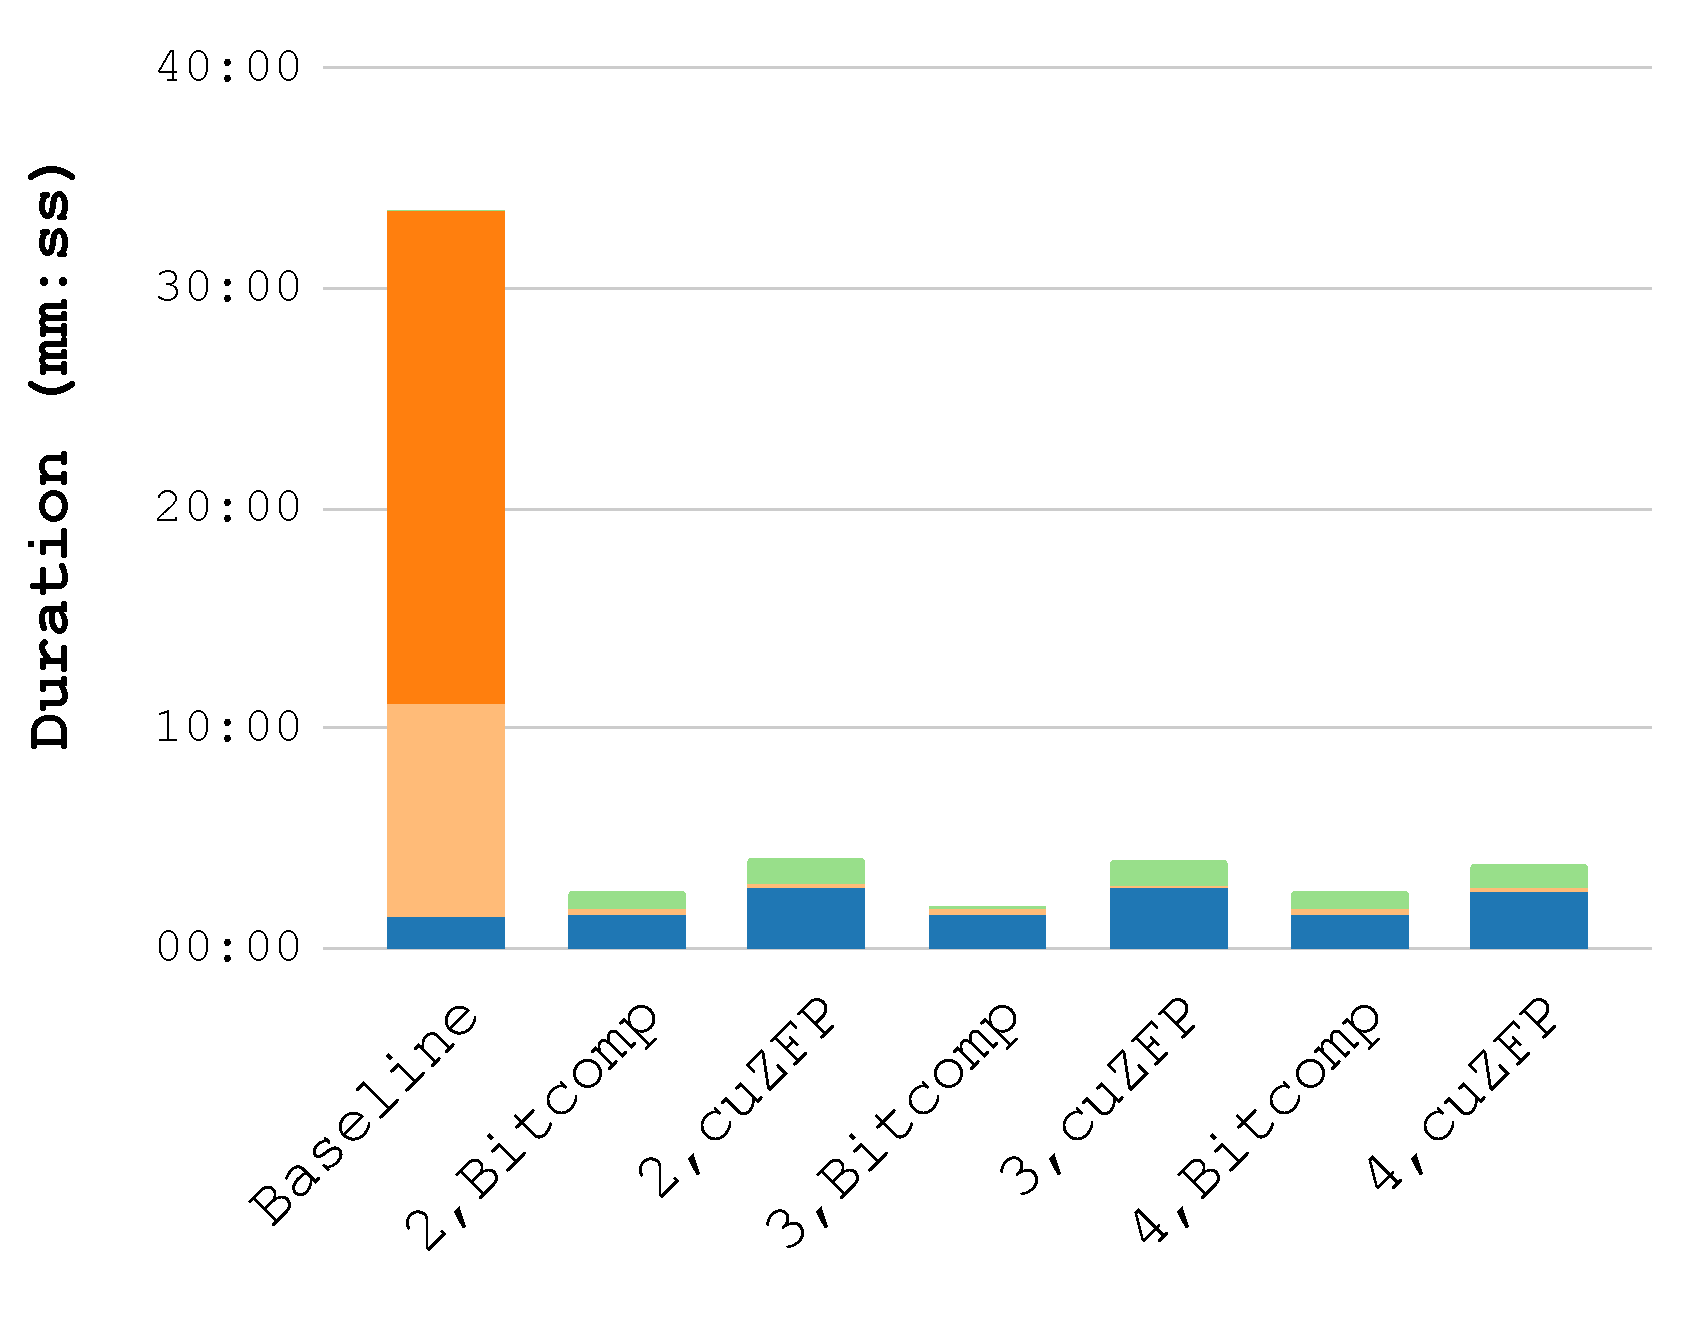
\includegraphics[width=\textwidth]{figures/gpuzip_breakdown/Figure7_a.pdf}
        \caption{\revolve}
        \label{fig:breakdown_revolve}
    \end{subfigure}%
    \hfill
    \begin{subfigure}{0.48\textwidth}
        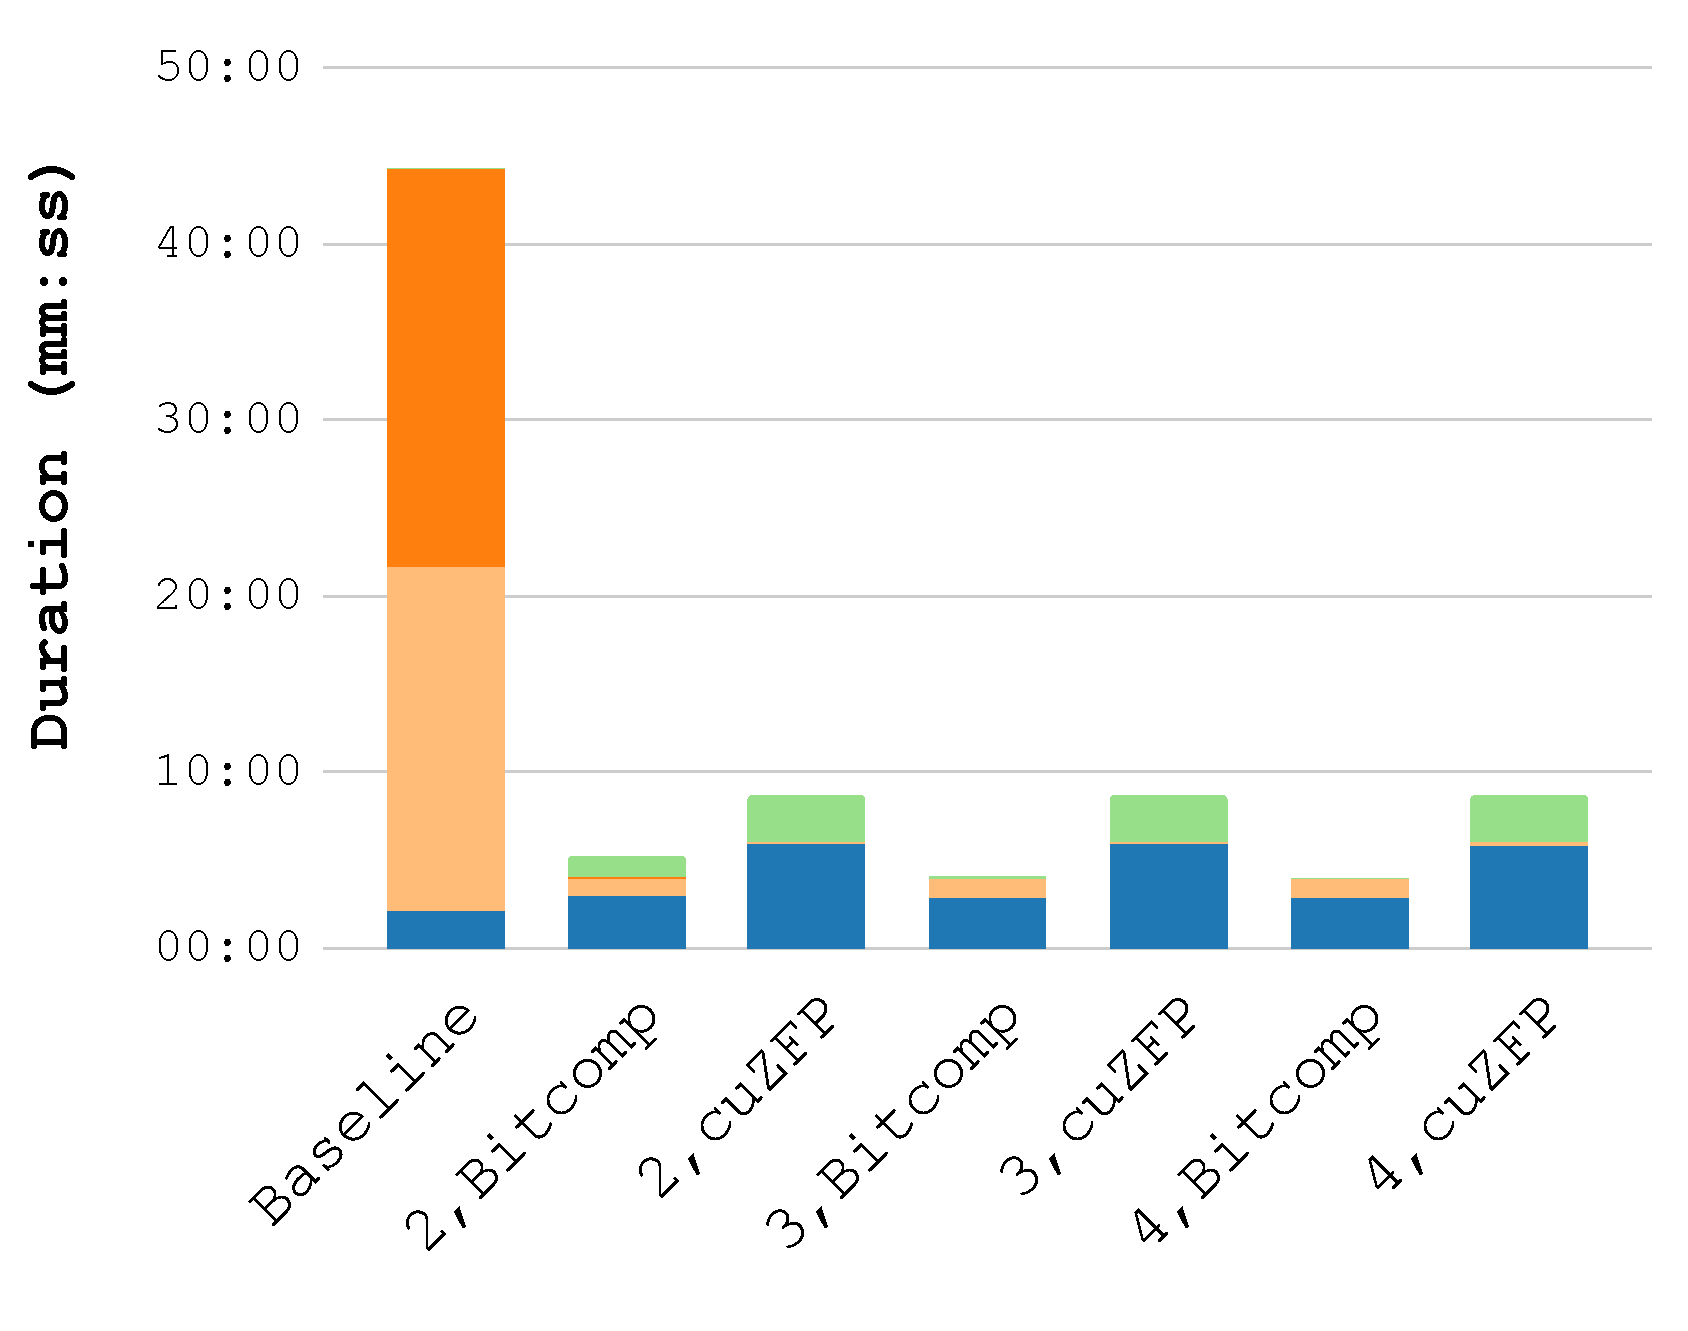
\includegraphics[width=\textwidth]{figures/gpuzip_breakdown/Figure7_b.pdf}
        \caption{\zcut}
        \label{fig:breakdown_zcut}
    \end{subfigure}
    \par\medskip  % Espaçamento entre linhas

    % Row 2: Chart (c)
    \begin{subfigure}{0.48\textwidth}
        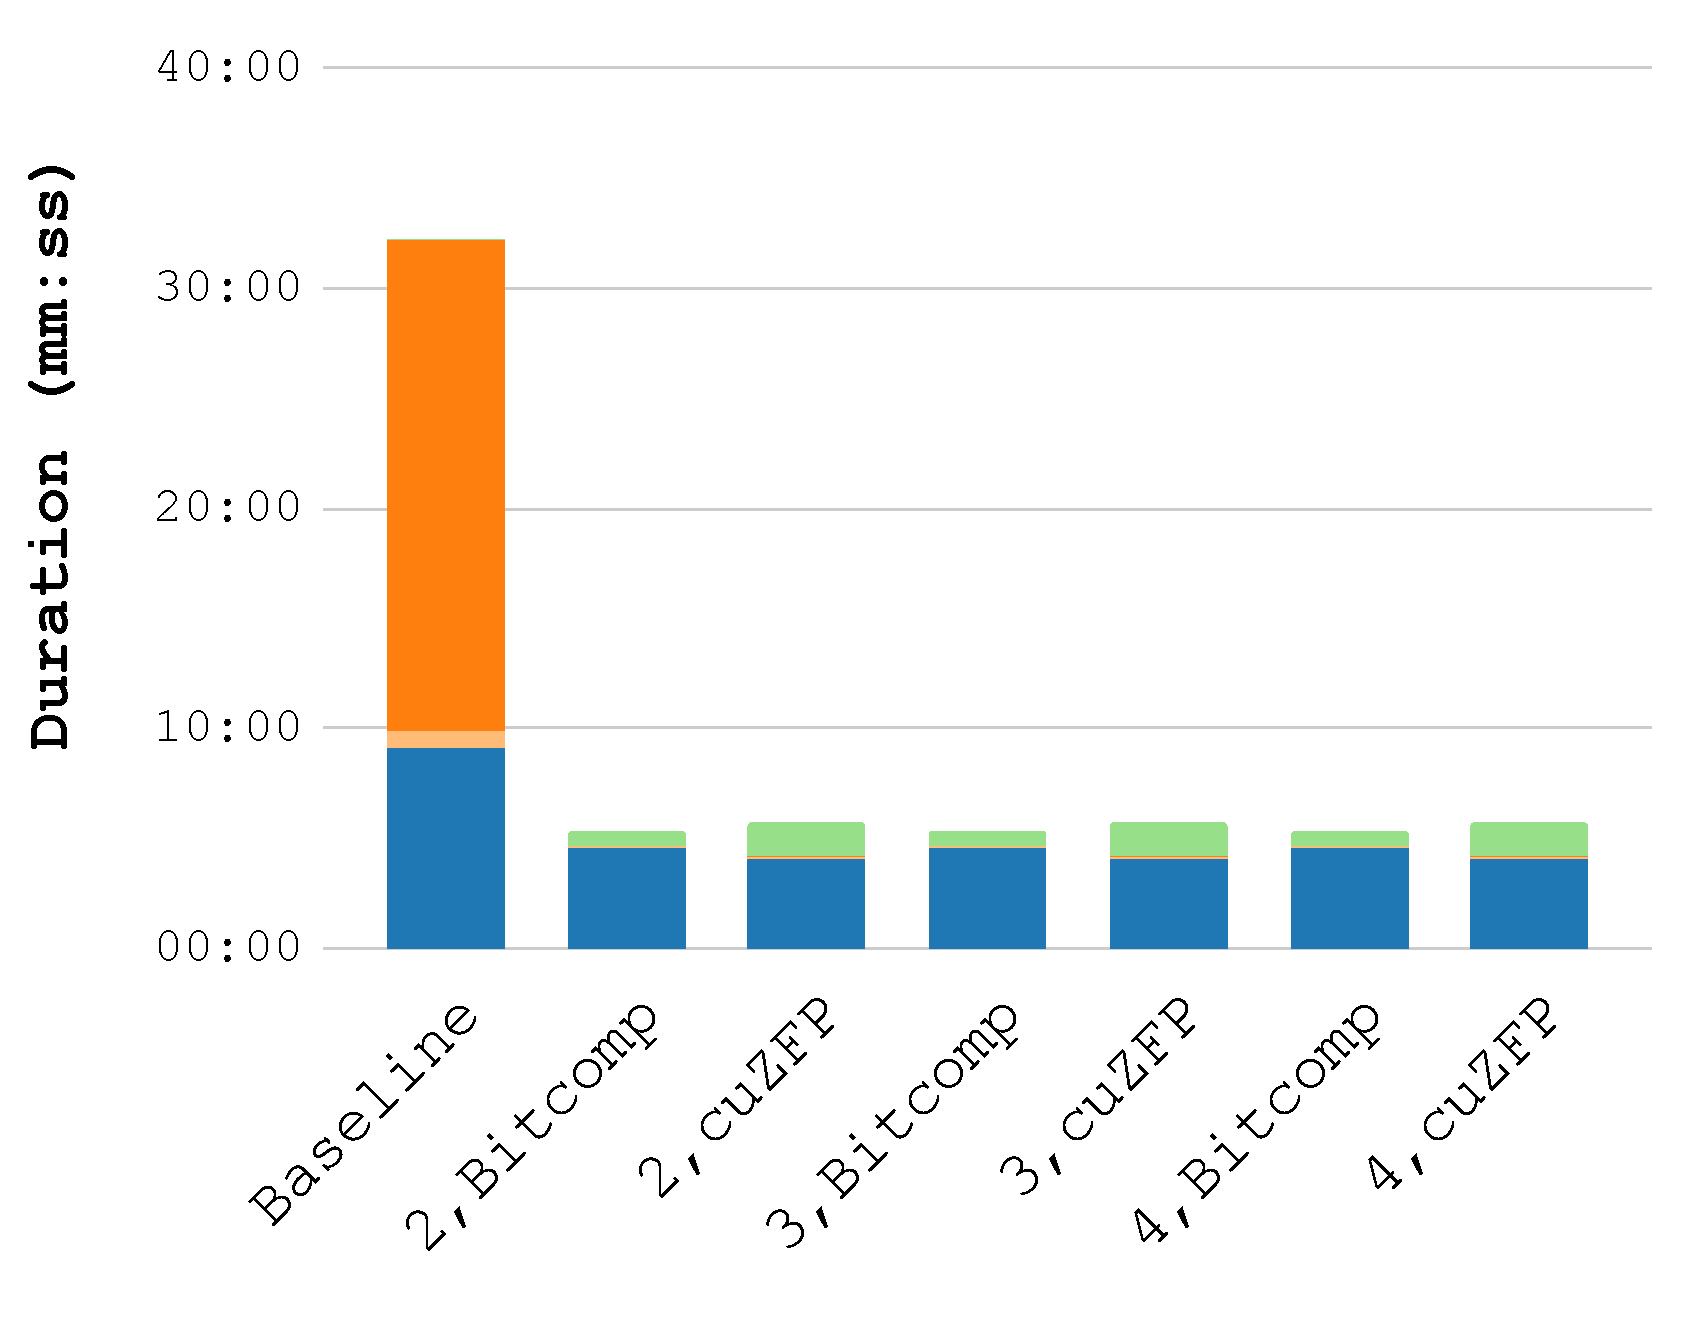
\includegraphics[width=\textwidth]{figures/gpuzip_breakdown/Figure7_c.pdf}
        \caption{\uniform}
        \label{fig:breakdown_uniform}
    \end{subfigure}

    \caption[Execution time breakdown (\checkpointprefetching + \compression)]{Execution time breakdown. The data corresponds to the Salt dataset for each \checkpointing library. Label (N,L) means N cache positions, compressing using the L library. (N, -) means N cache positions with no \compression.}
    \label{fig:breakdown}
\end{figure*}

\subsection{Memory Consumption}
\label{sec:comppref_mem}

As discussed in this chapter, \compression reduces data transfer time and significantly lowers memory consumption in the \cache. The required memory footprint is reduced since checkpoint data is compressed on the GPU before being stored in the cache. More minor memory requirements are advantageous for large datasets or systems (or programs) with limited available GPU memory, where fitting the required number of snapshots would otherwise be infeasible.

\rtab{prefcomp_mem} presents the GPU memory required by the \cache per GPU under different configurations. The table compares memory usage for each dataset when using: (a) no \compression, (b) \compression with Bitcomp, and (c) \compression with cuZFP. For Bitcomp, the memory allocation is based on the worst-case compression ratio observed during the warm-up phase. At the same time, cuZFP is configured to maintain a fixed compression ratio of $4\times$ (using \ttt{maxBits = 8}).

The results show that both compressors yield significant memory savings for all cache sizes and datasets compared to the uncompressed baseline. For instance, in the M3D\_Larger case with cache size 6, memory consumption drops from $\sim21.0GB$ (uncompressed) to $\sim8.1GB$ with Bitcomp and $\sim5.3GB$ with cuZFP.

\begin{table}[h!]
\centering
\begin{tabular}{|r|l|r|r|r|r|}
\hline
\rowcolor[HTML]{C0C0C0} 
\multicolumn{1}{|c|}{\cellcolor[HTML]{C0C0C0}\textbf{\begin{tabular}[c]{@{}c@{}}Cache\\ Size\end{tabular}}} &
  \multicolumn{1}{c|}{\cellcolor[HTML]{C0C0C0}\textbf{Compressor}} &
  \multicolumn{1}{c|}{\cellcolor[HTML]{C0C0C0}\textbf{\begin{tabular}[c]{@{}c@{}}Large\\ (GB)\end{tabular}}} &
  \multicolumn{1}{c|}{\cellcolor[HTML]{C0C0C0}\textbf{\begin{tabular}[c]{@{}c@{}}Marmousi3D\\ (GB)\end{tabular}}} &
  \multicolumn{1}{c|}{\cellcolor[HTML]{C0C0C0}\textbf{\begin{tabular}[c]{@{}c@{}}M3D\_Larger \\ (GB)\end{tabular}}} &
  \multicolumn{1}{c|}{\cellcolor[HTML]{C0C0C0}\textbf{\begin{tabular}[c]{@{}c@{}}Salt\\ (GB)\end{tabular}}} \\ \hline
\rowcolor[HTML]{EFEFEF} 
2 & -       & 1.0 & 0.8 & 7.0  & 0.9 \\ \hline
\rowcolor[HTML]{EFEFEF} 
2 & Bitcomp & 0.3 & 0.6 & 2.7  & 0.4 \\ \hline
\rowcolor[HTML]{EFEFEF} 
2 & cuZFP   & 0.2 & 0.2 & 1.7  & 0.3 \\ \hline
3 & -       & 1.6 & 1.2 & 10.5 & 1.4 \\ \hline
3 & Bitcomp & 0.4 & 0.5 & 4.0  & 0.6 \\ \hline
3 & cuZFP   & 0.7 & 0.3 & 2.6  & 0.4 \\ \hline
\rowcolor[HTML]{EFEFEF} 
4 & -       & 2.1 & 1.6 & 14.0 & 1.8 \\ \hline
\rowcolor[HTML]{EFEFEF} 
4 & Bitcomp & 0.5 & 0.6 & 5.4  & 0.8 \\ \hline
\rowcolor[HTML]{EFEFEF} 
4 & cuZFP   & 0.5 & 0.4 & 3.5  & 0.5 \\ \hline
5 & -       & 2.6 & 2.0 & 17.5 & 2.3 \\ \hline
5 & Bitcomp & 0.6 & 0.8 & 6.7  & 1.0 \\ \hline
5 & cuZFP   & 0.6 & 0.5 & 4.4  & 0.7 \\ \hline
\rowcolor[HTML]{EFEFEF} 
6 & -       & 3.1 & 2.4 & 21.0 & 2.8 \\ \hline
\rowcolor[HTML]{EFEFEF} 
6 & Bitcomp & 0.8 & 0.9 & 8.1  & 1.2 \\ \hline
\rowcolor[HTML]{EFEFEF} 
6 & cuZFP   & 0.7 & 0.6 & 5.3  & 0.7 \\ \hline
\end{tabular}
\caption[Memory consumption analysis (\checkpointprefetching + \compression)]{GPU Memory required by the \cache on each GPU in the system, considering no \compression (same as \rch{prefetch}) and the combination of \checkpointprefetching and \compression with Bitcomp and cuZFP.}
\label{tab:prefcomp_mem}
\end{table}


\subsection{Scalability}
\label{sec:comppref_scalability}

To assess the scalability of GPUZIP, the best-performing configuration, which combines Prefetching with Bitcomp compression, was tested in a distributed environment using multiple nodes. The parallelization strategy involved distributing the seismic shots among these nodes. The scalability figure shows that the observed speedup increases with the number of workers utilized. Ideally, this speedup should scale linearly with the number of nodes; however, due to the communication overhead in multi-node environments, actual performance tends to fall short of this theoretical maximum. A speedup of approximately 80\% of the expected performance based on the number of nodes was achieved, a trend consistently observed across all evaluated datasets.

Based on its demonstrated balance between compression ratio, memory usage, and performance, the experiments utilized the \revolve profile, configured with Bitcomp and a checkpoint cache size of 3. The scaling evaluation compared the baseline single-node execution against distributed runs with 2, 3, 4, and 6 nodes. OpenMP Cluster~\cite{ompc} coordinated the workload, with each worker responsible for processing a subset of the total shots.

\begin{figure}[h!]
    \centering
    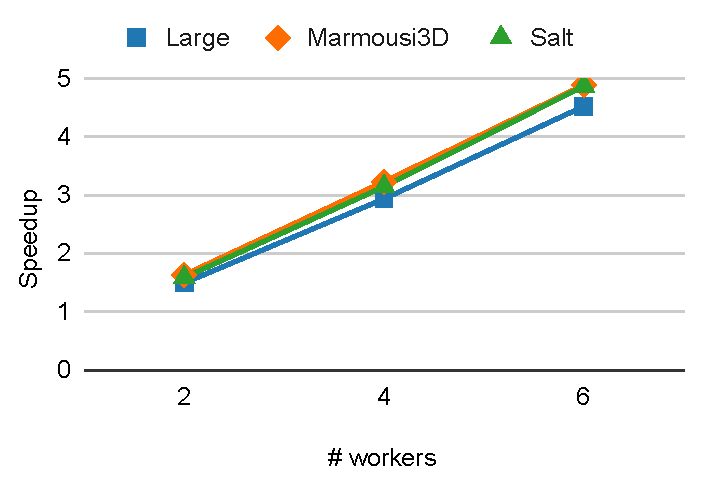
\includegraphics[width=0.7\linewidth,trim={5 10 0 10},clip]{figures/scalability.pdf}
    \caption[Speedup scalability in MNMG (\checkpointprefetching + \compression)]{Scalability of GPUZIP with the \revolve profile (Bitcomp + \cache size of 3) across varying numbers of workers (2, 3, 4, and 6) for the Large, Marmousi3D, and Salt datasets.}
    \label{fig:scalability}
\end{figure}

\chapter{GPUZIP as an API}
\label{ch:oss}

To conduct the experiments needed for this research, it was crucial to be flexible and swift in adjusting \compression parameters and algorithms to identify the optimal configuration for maximum performance. Achieving this adaptability required considerable software engineering efforts to consolidate all functionalities into a reusable and modular library; as a result, GPUZIP was developed.

%GPUZIP is an open-source software library licensed under the MIT License and available on GitHub~\cite{githubrepo} under the MIT license\footnote{\url{https://github.com/LSC-Unicamp/GPUZIP/blob/3c68c10e2074b4dc71cd20b36388567965e88ee9/LICENSE} -- Accessed Apr 24, 2025} written in C++/CUDA. It provides a framework for \checkpointing in GPU-based systems, incorporating \checkpointprefetching and GPU-based \compression support. The implementation of GPUZIP is organized around three main modules: Compression, Checkpointing Interface, and Prefetching.
GPUZIP is written in C++/CUDA and provides a framework for \checkpointing in GPU-based systems, incorporating \checkpointprefetching and GPU-based \compression support. The implementation of GPUZIP is organized around three main modules: Compression, Checkpointing Interface, and Prefetching. Its source code is available on GitHub~\cite{githubrepo}\footnote{Pending approval for open-sourcing under MIT license.}

This chapter is organized as follows: \rsec{ossmodules} introduces GPUZIP's main modules, APIs, and organization; \rsec{ossexample} provides an example of how GPUZIP can be integrated into a real-world application; \rsec{osslog} demonstrates how to set up logging in GPUZIP to help with troubleshooting and evaluation of the parameters; and finally, \rsec{gpuzipy} demonstrates an example of GPUZIPY, a Python wrapper for GPUZIP's Compressor module.

\section{The Software Architecture of GPUZIP}
\label{sec:ossmodules}
GPUZIP is architected around three modular components: Compression, Checkpointing Interface, and Prefetching. The Compression and Checkpointing modules are designed as standalone components, each exposing interfaces that allow them to be reused or integrated independently into other projects. The Prefetching module builds upon the same concept, but depends on Compression and Checkpointing Interface modules; however, it is still agnostic to the user's compressor or \checkpointing algorithm.

Using interfaces and abstract classes helps GPUZIP extend the library to support new compressors or \checkpointing algorithms, which can be introduced without modifying the core Prefetching logic, supporting clean and maintainable code evolution.

\subsection{Compression Module}

Following \rfig{compressoruml}, the Compression module defines a base abstract class (\sloppy{\verb|Compressor<C, D>|}) where ``\ttt{C}'' is the data type of the compressed data (e.g., integer) and ``\ttt{D}'' is the data type of the decompressed data (e.g., float). 

The \ttt{Compressor} interface provides public methods to compress and decompress data on the GPU.

\begin{itemize}
    \item \textbf{\ttt{Compress(...)}}: This function receives a pointer to uncompressed GPU data (\ttt{in}) and writes the compressed result to the output buffer (\ttt{out}). It returns the real size of the compressed data.
    \item \textbf{\ttt{Decompress(...)}}: This function receives a pointer to compressed GPU data (\ttt{in}) and writes the decompressed result to the output buffer (\ttt{out}).
\end{itemize}

Concrete implementations inherit from \sloppy{\verb|Compressor<C, D>|} abstract class to encapsulate the specific logic of each compression backend, such as \sloppy{\verb|CompressorZFP|}, \sloppy{\verb|CompressorCuSZp|}, and \sloppy{\verb|CompressorBitcomp|}. Each child class overrides the ``\ttt{compress}'' and ``\ttt{decompress}'' \tit{virtual} methods, adapting them to the behavior and constraints of the respective compression library.

\begin{figure}
  \centering
  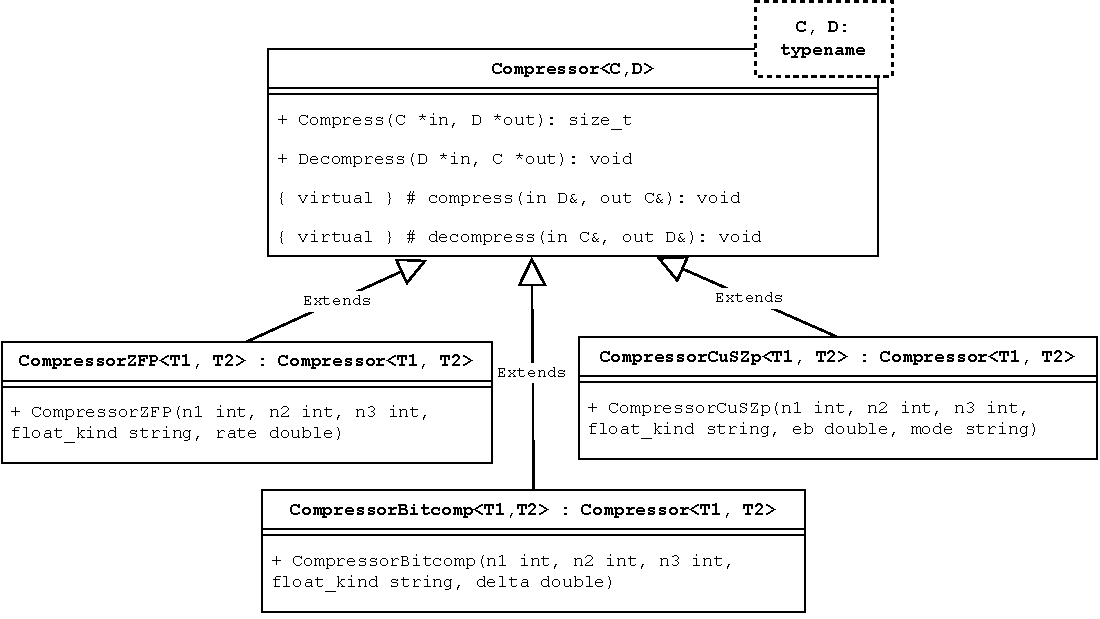
\includegraphics[width=1\linewidth,trim={0 0 0 0},clip]{figures/oss/compressor_uml.pdf}
  \caption[Compressor module class diagram]{Compressor module class diagram (UML).}
  \label{fig:compressoruml}
\end{figure}


\subsection{Checkpointing Interface Module}

The second module of GPUZIP is the Checkpointing Interface, which defines a unified abstraction layer to decouple the application logic from the used \checkpointing algorithm. This design allows users to switch between different \checkpointing strategies, such as \revolve, \zcut, or custom implementations, without modifying the user's code.

\rfig{checkpointinguml} illustrates the internal architecture of this module. At its core, it includes an enumeration named \ttt{ActionType} and a \texttt{Action} structure, standardizing the semantics of \checkpointing operations across all implementations. This standard representation enables consistent communication between the user's code and the \checkpointing algorithm, regardless of the specific algorithm.

The central abstraction is the \texttt{Checkpointing} class, an abstract base class that exposes public methods. The most important, from the user's perspective, is the \texttt{GetAction()} method: it returns an \texttt{Action} object indicating the type of operation to perform (e.g., \texttt{ACTION\_SAVE}, \texttt{ACTION\_RESTORE}, \texttt{ACTION\_BACKWARD}) and the timestep at which it should occur.

Specific \checkpointing algorithms are implemented by extending the \texttt{Checkpointing} class. For instance, \texttt{RevolveCheckpointing} inherits from \texttt{Checkpointing} and encapsulates the logic of the \revolve algorithm.

% This clean separation of concerns makes the \ttt{Checkpointing} a cornerstone of GPUZIP's flexibility. It ensures that new checkpointing algorithms can be integrated seamlessly, promoting extensibility and minimizing the integration overhead on experimentation or the user's source code.


\begin{figure}
  \centering
  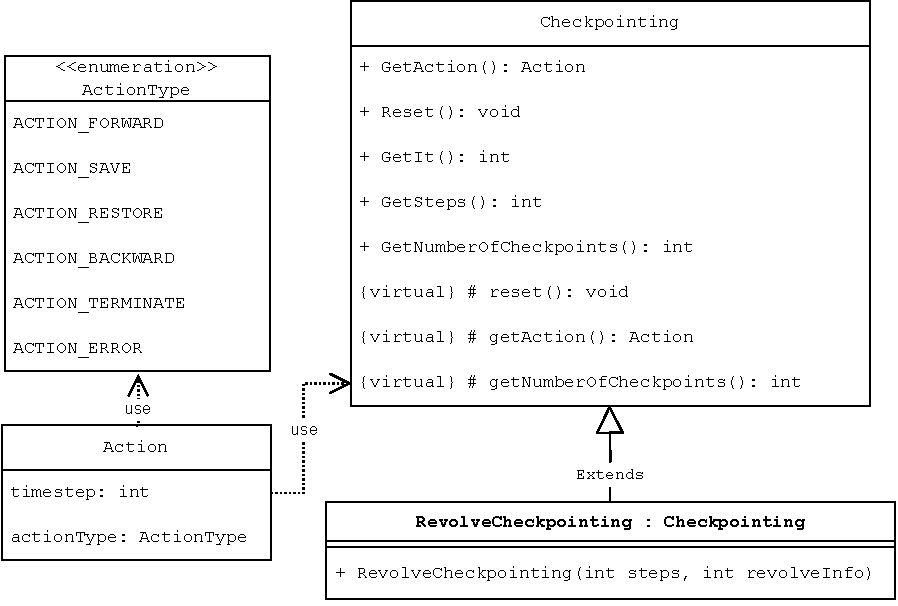
\includegraphics[width=0.9\linewidth,trim={0 0 0 0},clip]{figures/oss/checkpointing_uml.pdf}
  \caption[Checkpointing module class diagram]{Checkpointing module class diagram (UML)}
  \label{fig:checkpointinguml}
\end{figure}

\subsection{Prefetching Module}

The Prefetching module implements the core logic of the prefetching mechanism and checkpoint data \compression, as detailed in \rch{prefetch}. This module depends on the \texttt{Checkpointing} and \texttt{Compressor} interfaces but remains agnostic to the specific libraries being used. 

As illustrated in \rfig{prefetchuml}, the \texttt{Prefetch} class internally maintains two key components: the \cache and the \pav (PAV), which are protected attributes. All public methods operate on a unified abstraction of the data fields to be checkpointed, represented by the \texttt{Field\_t} structure. This structure includes a pointer to a GPU-allocated buffer (\texttt{void*}), the field size in bytes, and the dimensions of the 3D data (n1, n2, n3).

The core functionality is exposed via the \texttt{Save(...)} and \texttt{Retrieve(...)} methods. These methods accept \texttt{Field\_t} structures for the current and previous fields and optional compressor instances when \compression is used. 

The \psa (PSA), responsible for computing the PAV, is implemented as a \texttt{virtual} method, which enables the module to be extended with custom PSA implementations by subclassing and overriding \texttt{setup()} method.

Once PSA computes the PAV, the user must call \texttt{Dispatch()} in every iteration. This method checks if a prefetch action is scheduled for the current timestep and, if so, initiates the asynchronous memory transfer.

The module also provides a \texttt{Reset()} method to reinitialize all internal counters and clear the cache and PAV at the beginning of a new shot.

The \texttt{Prefetch} class is the central component for enabling prefetching in GPUZIP and adheres to the same object-oriented architecture as the \texttt{Checkpointing} and \texttt{Compressor} modules. For cases where prefetching is not desired, GPUZIP also includes a minimalistic implementation named \texttt{CheckpointingOnly}, which supports only saving and restoring snapshots, optionally with \compression. This class serves as the experimental baseline for evaluating the benefits of the prefetching mechanism later integrated into \awave.


\begin{figure}
  \centering
  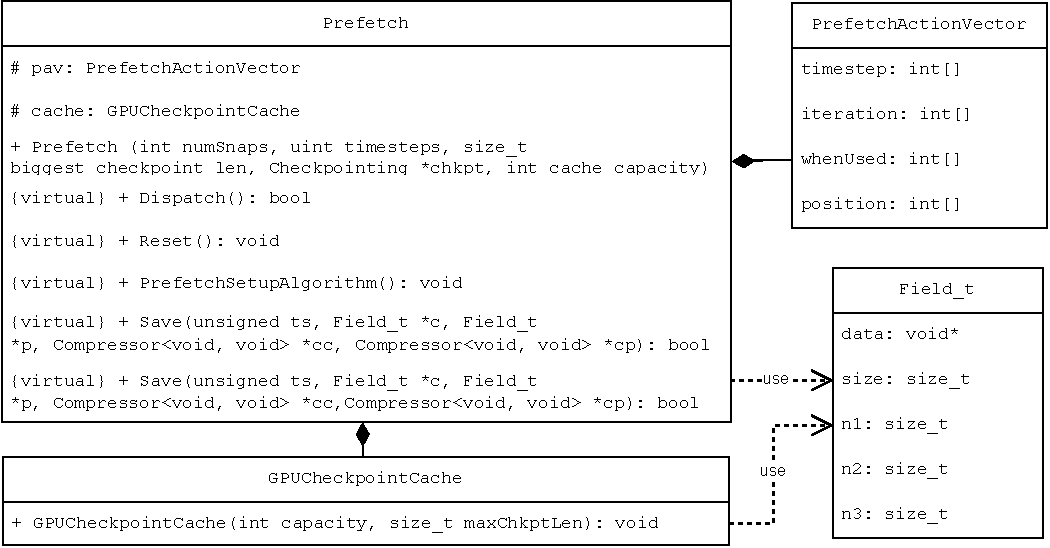
\includegraphics[width=1\linewidth,trim={0 0 0 0},clip]{figures/oss/prefetch_uml.pdf}
  \caption[Prefetching module class diagram]{Prefetching module class diagram (UML).}
  \label{fig:prefetchuml}
\end{figure}


\section{GPUZIP Usage}
\label{sec:ossexample}
In a nutshell, GPUZIP can offer \checkpointing with prefetch and compression into an adjoint computation loop (such as RTM) in an immutable code that does not depend on the configuration; the users do not need to change their source code because they want to experiment with other compressor libraries, use another \checkpointing library or use a bigger checkpoint cache.~\rlst{cudaexample} shows how the integration is performed in a single GPU environment through a modular design that isolates configuration and functionality into builders and abstract interfaces.


\begin{figure}[h!]
\centering
\begin{lstlisting}[language=C++, caption={Example of an adjoint computation (such as RTM) integration with GPUZIP}, label={lst:cudaexample}]
#include "prefetch/Prefetch.cuh"
#include "prefetch/Checkpointing.hpp"
#include "common/GPUZIPBuilders.cpp"
#include "common/GPUZIPConfig.h"

Field_t BuildField(your_data_t* d) {
    size_t size = d->n1 * d->n2 * d->n3 * sizeof(float);
    return Field_t{d->n1, d->n2, d->n3, d->data, size};
}

void adjoint(gpuzip_config_t *cfg, your_data_t *data, int steps) {
    Checkpointing *chkpt = CheckpointingBuilder(cfg, steps);
    Prefetch *prefetch = PrefetchBuilder(cfg, steps, chkpt);

    for (int shot = 0; shot <= data->shots; ++shot) {
        bool done = false;
        prefetch->Setup();
        do {
            Action act = chkpt->GetAction();
            prefetch->Dispatch(chkpt->GetIt());

            if (act.actionType == ACTION_SAVE) {
                Field_t c = BuildField(data->curr);
                Field_t p = BuildField(data->prev);
                auto cc = CompressorBuilder(cfg, c.n1, c.n2, c.n3);
                auto cp = CompressorBuilder(cfg, p.n1, p.n2, p.n3);
                prefetch->Save(act.ts, &c, &p, cc.get(), cp.get());
            }
            if (act.actionType == ACTION_FORWARD)
                forward_computation(act.ts, data);
            if (act.actionType == ACTION_BACKWARD)
                backward_computation(act.ts, data);
            if (act.actionType == ACTION_RESTORE) {
                Field_t c = BuildField(data->curr);
                Field_t p = BuildField(data->prev);
                auto cc = CompressorBuilder(cfg, c.n1, c.n2, c.n3);
                auto cp = CompressorBuilder(cfg, p.n1, p.n2, p.n3);
                prefetch->Retrieve(act.ts, &c, &p, cc.get(), cp.get());
            }
            if (act.actionType == ACTION_TERMINATE)
                done = true;
            if (act.actionType == ACTION_ERROR)
                done = true;
        } while (!done);
    }
    prefetch->Free();
}
\end{lstlisting}
\end{figure}

The integration core begins in lines 12-13, where \sloppy{\verb|CheckpointingBuilder|} and \sloppy{\verb|PrefetchBuilder|} instantiate the appropriate checkpointing and caching strategy based on the parameters provided in \sloppy{\verb|gpuzip_config_t|}. This configuration \ttt{struct} can define the cache size, the compressor to be used (Bitcomp, cuSZp, cuZFP, etc.), and the \checkpointing algorithm (\revolve, \zcut, etc.) without requiring any further changes to the main application code.

Within the main shot loop (line 16), GPUZIP orchestrates the prefetching and \checkpointing logic: \sloppy{\verb|prefetch->Setup()|} (line 17) runs the \psa that will define \pav, making the system able to prefetch. In the inner loop (lines 18–44), the application receives \checkpointing decisions from \sloppy{\verb|chkpt->GetAction()|} (line 19), which returns the next required operation, such as \save, \restore, \fwd or \bwd, along with the associated timestep.

The \save operation (lines 22–28) sets up \sloppy{\verb|Field_t|} with the current and previous values computed in the last iteration, and then the compressor for the respective fields. Similarly, \restore (lines 33–39) retrieves the checkpoint data using the same pattern. \fwd and \bwd computation kernels (lines 29-32) are untouched, demonstrating that GPUZIP integrates into the existing simulation loop without disrupting computational logic.

Finally, the user can \sloppy{\verb|prefetch->Free()|} (line 46) and release the host and GPU memory allocated by GPUZIP.

The modular design allows developers to change \checkpointing strategies, compressors, or cache configurations entirely through the gpuzip\_config\_t structure, enabling rapid experimentation and tuning without modifying the simulation code. This design philosophy is critical for large-scale scientific codes, where maintainability and extensibility are essential.

%A demonstration with multi-GPU is very similar to that and can be found in the GPUZIP documentation\footnote{\url{https://github.com/LSC-Unicamp/GPUZIP/blob/main/docs/CppCudaExamples.md} -- Accessed May 26, 2025}.
A demonstration with multi-GPU and the required build configuration and dependencies to incorporate GPUZIP into a real-world project can be found in the Appendix~\ref{appendix:gpuzip}.

\section{Logging: Evaluating and Troubleshooting}
\label{sec:osslog}

GPUZIP provides several mechanisms to aid in evaluating performance and diagnosing issues with its configuration and execution.

GPUZIP offers a static utility class named \texttt{GPUZIPLogger} for more detailed logging. Enabling the performance trace feature via \sloppy{\verb|GPUZIPLogger::PerfTraceSwitch(true);|} allows users to see information about internal structures such as the length and memory usage of the \cache and \pool.

GPUZIPLogger also supports configurable log levels, which are essential for troubleshooting. Logging verbosity can be set using \sloppy{\verb|GPUZIPLogger::SetLevel(int)|}, with supported levels being: \texttt{0=DEBUG}, \texttt{1=INFO}, \texttt{2=WARN}, and \texttt{3=ERROR}. At the \texttt{DEBUG} level, GPUZIP prints detailed trace messages, including internal \cache states and every action the prefetching mechanism takes. The \texttt{INFO} level outputs general configuration details and includes messages from the \texttt{WARN} and \texttt{ERROR} levels, which report abnormal behavior such as misconfigurations or failures in memory transfers.

Invoking \sloppy{\verb|prefetch->Report()|} method at the end of the run. It provides a quick overview of the current prefetching configuration's effectiveness. This lightweight method prints useful statistics to the console, including the number of cache hits and misses, as well as the number of cache misses successfully avoided by prefetching.

Additionally, GPUZIP supports integration with NVIDIA's NSight profiling tools through the NVTX (NVIDIA Tools Extension) library. By defining the macro \ttt{USE\_NVTX} at compile time, developers can insert NVTX markers into the execution trace, allowing for fine-grained performance analysis. For example, this can be enabled in a \texttt{CMakeLists.txt} file with \texttt{add\_definitions(-DUSE\_NVTX)}.

\section{GPUZIPy: A Python Wrapper for GPUZIP}
\label{sec:gpuzipy}

GPUZIPy is a Python wrapper for GPUZIP designed to integrate GPU-based \compression into Python applications. Currently, only the Compressor module is exposed to Python, enabling seamless compression and decompression using Python-based scientific computing stacks.

The wrapper is built using \texttt{pybind11}\footnote{\url{https://github.com/pybind/pybind11} -- accessed Apr 25, 2025}, a tool to expose C++ types in Python and vice-versa, and operates on \texttt{cuPy}\footnote{\url{https://cupy.dev/} -- accessed Apr 25, 2025}, a NumPy-compatible\footnote{\url{https://numpy.org/} -- accessed Apr 25, 2025} array library allowing GPU memory management and CUDA computation from Python.

To use GPUZIPy, data originally residing in the host (as a NumPy array) must first be transferred to the GPU using \texttt{cuPy}. Once on the GPU, the compression and decompression routines can be invoked using the interfaces provided by GPUZIPY. \rlst{gpuzipy} shows a basic example of setting up a compressor, transferring data to the GPU, and invoking the compression and decompression methods.

The example starts by importing necessary modules (\texttt{gpuzipy}, \texttt{cupy}, and \texttt{numpy}). A compressor is instantiated based on the configuration (\texttt{Bitcomp} or \texttt{cuZFP}), as shown in lines 10-23. Line 27 creates a Numpy array for exemplification and transfers the input data from host to device using \texttt{cuPy} in line 30. Line 31 obtains the estimated compressed buffer size to allocate memory for receiving the compressed data in line 32. Finally, line 33 compresses the data using the unified \texttt{compress(...)} helper function. The same approach applies to decompression with the \texttt{decompress(...)} helper (lines 36-37).

\begin{minipage}{\linewidth}
\begin{lstlisting}[language=Python, caption={Example of using GPUZIPY to compress data on the GPU}, label={lst:gpuzipy}]
from gpuzipy import CompressorZFP, CompressorBitcomp, compressed_buffer_size, compressed_buffer_max_size, compress, decompress
import cupy as cp
import numpy as np
import math

BITCOMP = 1; CUZFP = 2

n1 = 100; n2 = 100; n3 = 100

def build_compressor(selected_compressor):
    compressor = None

    if selected_compressor == BITCOMP: 
        ERROR_BOUND = 2
        ALGO_DEFAULT = 'default'
        delta=1e-8
        compressor = CompressorBitcomp(n1, n2, n3, ERROR_BOUND, 0.0, 0.0, delta, 'float', ALGO_DEFAULT)
    
    elif selected_compressor == CUZFP:
        max_bits = 8
        compressor = CompressorZFP(n1, n2, n3, 'float', max_bits)

    return compressor

# Setup phase
compressor = build_compressor(CUZFP)
h_uncompressed = np.random.rand(n1, n2, n3).astype(np.float32)

# Compression phase
d_uncompressed = cp.asarray(h_uncompressed)
estimated_size = compressed_buffer_max_size(compressor)
d_compressed_ptr = cp.cuda.malloc_async(estimated_size)
compress(compressor, d_uncompressed.data.ptr, d_compressed_ptr.ptr)

# Decompression phase
d_decompressed = cp.empty((n1, n2, n3), dtype=np.float32)
decompress(compressor, d_compressed_ptr.ptr, d_decompressed.data.ptr)
\end{lstlisting}
\end{minipage}

\chapter{Conclusion}
\label{ch:conclusion}

This research aimed to improve and accelerate \checkpointing in heterogeneous computing systems with GPUs by reducing GPU-host communication overhead through prefetching techniques and data \compression.

Throughout this dissertation, the Research Questions (RQ) outlined in \rch{intro} were addressed through the development and validation of the Specific Objectives (SO).

RQ1 asked whether \checkpointing algorithms provide sufficient hinting to support an effective prefetching mechanism. \rch{prefetch} answered this question addressing the SO1, SO2 and SO3. It described the implementation of the \cache structure, which includes a synchronization mechanism and an LRU eviction policy (SO1). This structure proved essential given that \checkpointing algorithms tend to reuse snapshots. The \psa was also implemented to identify when a \tit{cache miss} would occur and to schedule a prefetch in advance (SO2).

SO3 involved testing multiple cache sizes (2 to 6) across all \checkpointing algorithms to determine the most effective configuration. Results showed that \revolve is the most sensitive to cache size due to its frequent reuse of snapshots. In contrast, \zcut suffers from cache saturation due to high snapshot density, and \uniform requires less cache due to the ample time between \restore actions, making two slots sufficient.

At this stage, speedups of up to $3.4\times$ for \revolve, $1.7\times$ for \zcut, and $2.3\times$ for \uniform were achieved by reducing (though not eliminating) PCIe blocking time. No cache misses occurred; however, in some cases, the prefetched data did not arrive in time, resulting in residual communication latency.

Thus, the answer to RQ1 is that \checkpointing algorithms provide enough hinting for prefetching all required data. Despite this, timing limitations prevent prefetching alone from eliminating PCIe transfer stalls.

RQ2, addressed in \rch{compress} through SO4 and SO5, evaluated whether compression could reduce PCIe overhead without compromising output quality. Available GPU-based compressors were assessed, and the best performers, cuZFP and NVIDIA's Bitcomp, were selected after warmup testing. Their optimal parameters were determined and used throughout the experiments.

Compression alone achieved speedups with Bitcomp for \revolve and \zcut due to its higher compression ratios and faster throughput, reaching up to $4.57\times$ and $6.50\times$ respectively. For \uniform, Bitcomp outperformed on the Large dataset, while cuZFP delivered better results for Marmousi3D and Salt (up to $5.09\times$). Compression also enabled more snapshots to be stored, which reduced recomputation in \uniform. Additionally, both compressors preserved image quality, as confirmed by PSNR, SSIM metrics, and visual inspection. Therefore, RQ2 is answered: compression reduces PCIe overhead without significantly degrading the quality of the results.

RQ3, addressed in \rch{comppref} through SO6, evaluated the combination of prefetching and compression. GPUZIP integrates both mechanisms, using the \cache and \psa alongside the compressor modules. The combined approach achieved speedups up to $5.1\times$ for \revolve, $8.8\times$ for \zcut, and $5.8\times$ for \uniform, outperforming each technique in isolation.

\rch{comppref} also demonstrated that compression enhances prefetching by reducing transfer size, making transferring faster, and enabling larger caches, even on GPUs with limited memory. Prefetching complements compression by hiding \htd transfer latency, which would otherwise be synchronous.

In \rch{oss}, the research is wrapped into GPUZIP~\cite{githubrepo}\footnote{Pending approval for open-sourcing under MIT license.}, a reusable and extensible library with a Python API. GPUZIP made experimentation efficient by allowing multiple configurations to be tested without changing the \awave source code. GPUZIP invites contributions and adoption in other scientific domains.

As an academic contribution, the GPUZIP research was presented in a poster at Super Computing 2023~\cite{sc23}, a paper was accepted for the EUROPAR 2024 conference~\cite {europar}, and an article was published in the IJHPCA in 2025~\cite{ijhpca}. 

Finally, this work opens avenues for future research, such as applying GPUZIP to machine learning workloads, especially as \zcut was initially proposed for that domain, or extending its use to multi-tiered storage systems involving SSDs.



% As referências:
\bibliographystyle{plain}
\bibliography{ic-tese-v3}


% Os anexos, se houver, vêm depois das referências:
\appendix
\chapter{Itegrating GPUZIP in a C++/CUDA Project}
\label{appendix:gpuzip}

This appendix provides detailed instructions for integrating GPUZIP with C++ and CUDA projects. It describes the required dependencies, how to configure GPUZIP within a \texttt{CMakeLists.txt} file, and how to manage GPUZIP's compilation flags. Furthermore, it includes a practical example demonstrating GPUZIP's usage in a multi-GPU adjoint computation scenario.

The following versions were tested for compatibility:

\begin{itemize}
    \item CMake 3.22
    \item Make 4.2
    \item NVCC 10.1
    \item CUDA 12.2
    \item cuZFP (refer to the \textit{Installing cuZFP} tutorial)
\end{itemize}

Alternatively, the Docker image \texttt{maltempi/awave-dev:ompc} can be used to simplify the environment setup.

\section{Example of \texttt{CMakeLists.txt} Configuration}

\begin{lstlisting}[language=CMake, caption={Example of CMake configuration to include GPUZIP}, label={lst:cmake}]
set(CMAKE_CXX_STANDARD 17)

include_directories(./GPUZIP/src/Prefetch/include)
include_directories(./GPUZIP/src/Compressor/include)
add_library(cuda_utils ./GPUZIP/src/Compressor/cuda_utils.cu)

option(USE_NVTX "GPUZIP use NVTX (nsight) tracing." OFF)
if (USE_NVTX)
    add_definitions(-DUSE_NVTX)
endif()

# Enable ZFP compression
option(ZFP "Includes cuZFP as an available compressor." ON)
if (ZFP)
    add_definitions(-DZFP)
    include_directories(/opt/zfp/include)

    if (NOT DEFINED CMAKE_CUDA_FLAGS)
        set(CMAKE_CUDA_FLAGS "")
    endif()
    set(CMAKE_CUDA_FLAGS "${CMAKE_CUDA_FLAGS} --extended-lambda --expt-relaxed-constexpr -Wno-deprecated-declarations")

    target_link_libraries(awave3d-decom
        /opt/zfp/lib/libzfp.so
        /opt/zfp/lib/libzfp.so.1
        /opt/zfp/lib/libzfp.so.1.0.0
        -lnvToolsExt
        -lcuda
        -lcusparse)
endif()

# Enable NVCOMP BITCOMP
option(NVCOMP_BITCOMP "Includes NVIDIA Bitcomp as an available compressor." ON)
if (NVCOMP_BITCOMP)
    add_definitions(-DNVCOMP_BITCOMP)
    message(STATUS "Using NVCOMP BITCOMP")

    include(FetchContent)

    FetchContent_Declare(
        NVCOMP_BITCOMP
        DOWNLOAD_EXTRACT_TIMESTAMP false
        URL https://developer.download.nvidia.com/compute/nvcomp/2.6.1/local_installers/nvcomp_2.6.1_x86_64_12.x.tgz
        URL_HASH SHA256=ac4834397291f245578af959694e816d96f80036eac50b5f24b113dee5b54225
        TLS_VERIFY false
    )
    FetchContent_MakeAvailable(NVCOMP_BITCOMP)

    FetchContent_GetProperties(NVCOMP_BITCOMP SOURCE_DIR NVCOMP_SRC_DIR)
    message(STATUS "NVCOMP_SRC_DIR: ${NVCOMP_SRC_DIR}")

    list(APPEND CMAKE_PREFIX_PATH "${NVCOMP_SRC_DIR}/lib/cmake/nvcomp")

    message(STATUS "CMAKE_PREFIX_PATH: ${CMAKE_PREFIX_PATH}")

    find_package(nvcomp REQUIRED CONFIG PATHS "${NVCOMP_SRC_DIR}/lib/cmake/nvcomp")

    target_link_libraries(awave3d-decom
        nvcomp::nvcomp_bitcomp
        cuda_utils
        -lnvToolsExt
        -lcuda
        -lcusparse)
endif()

# Enable cuSZp compression
option(CUSZP "Includes cuSZp as an available compressor." ON)

if (CUSZP)
    add_definitions(-DCUSZP)
    message("Using CUSZP")
    include(FetchContent)

    FetchContent_Declare(
        cuszp
        GIT_REPOSITORY https://github.com/szcompressor/cuSZp.git
        GIT_TAG cuSZp-V1.1
    )
    FetchContent_MakeAvailable(cuszp)
    target_link_libraries(awave3d-decom
      cuSZp
      cuda_utils
      -lnvToolsExt
      -lcuda
      -lcusparse)
endif()
\end{lstlisting}

\section{Managing GPUZIP Compilation Flags}

By default, GPUZIP enables all available compressors. For production environments, it is recommended to disable unused compressors to reduce binary size and simplify deployment. The flags \texttt{CUZFP}, \texttt{CUSZP}, and \texttt{BITCOMP} control whether the respective compressors are enabled. Additionally, the \texttt{USE\_NVTX} flag enables internal instrumentation with NVIDIA NSight.

\begin{lstlisting}[language=bash, caption={Example of CMake flags usage}, label={lst:cmakeflags}]
## Default configuration (all compressors enabled)
cmake 

## Disabling cuZFP and cuSZP
cmake -DCUZFP=0 -DCUSZP=0

## Disabling Bitcomp only
cmake -DBITCOMP=0

## Enabling NVTX tracing
cmake -DUSE_NVTX=1
\end{lstlisting}

\section{Example: Multi-GPU Adjoint Computing with Prefetch and Compression}

The following example illustrates the usage of GPUZIP in a multi-GPU adjoint computation setup. The implementation is agnostic to the specific compressor or checkpointing algorithm used.

The variable \texttt{your\_data\_t} symbolizes user-defined data structures representing current and previous fields. The fields are partitioned across multiple GPUs.

All configurable parameters for GPUZIP are encapsulated within the \texttt{gpuzip\_config\_t} structure, defined in \texttt{Prefetch/include/common/GPUZIPBuilders.cpp}.

\begin{lstlisting}[language=C++, caption={Example of multi-GPU adjoint computation with GPUZIP}, label={lst:adjoint}]
#include "prefetch/Prefetch.cuh"
#include "prefetch/Checkpointing.hpp"
#include "common/GPUZIPBuilders.cpp"
#include "common/GPUZIPConfig.h"

void adjoint(gpuzip_config_t *gpuzip_config, your_data_t *data, int num_gpus) {
    GPUZIPLogger::SetLevel(gpuzip_config->log_level);
    GPUZIPLogger::PerfTraceSwitch(gpuzip_config->enable_performance_log);

    int steps = afd->nt;
    bool useCompression = gpuzip_config->compressor > 0;

    Checkpointing *chkpt = CheckpointingBuilder(gpuzip_config, steps);
    int snaps = chkpt->GetNumberOfCheckpoints();

    Prefetch *prefetch[num_gpus];
    for (int d = 0; d < num_gpus; d++) {
        size_t n1 = std::max(data->curr->devices[d].n1, data->prev->devices[d].n1);
        size_t n2 = std::max(data->curr->devices[d].n2, data->prev->devices[d].n2);
        size_t n3 = std::max(data->curr->devices[d].n3, data->prev->devices[d].n3);
        prefetch[d] = PrefetchBuilder(gpuzip_config, steps, chkpt); 
    }

    for (int shot = 0; shot <= data->shots; shot++) {
        for (int d = 0; d < num_gpus; d++) {
            cudaSetDevice(d);
            prefetch[d]->Setup();
        }

        chkpt->Reset();
        bool terminate = false;

        do {
            Action action = chkpt->GetAction();

            for (int d = 0; d < num_gpus; d++) {
                cudaSetDevice(d);
                prefetch[d]->Dispatch(chkpt->GetIt());
            }

            if (action.actionType == ACTION_SAVE) {
                for (int d = 0; d < num_gpus; d++) {
                    cudaSetDevice(d);

                    Field_t curr = {
                        .n1 = data->curr->devices[d].n1,
                        .n2 = data->curr->devices[d].n2,
                        .n3 = data->curr->devices[d].n3,
                        .data = data->curr->devices[d].data,
                        .size = data->curr->devices[d].n1 * data->curr->devices[d].n2 * data->curr->devices[d].n3 * sizeof(float)
                    };

                    Field_t prev = {
                        .n1 = data->prev->devices[d].n1,
                        .n2 = data->prev->devices[d].n2,
                        .n3 = data->prev->devices[d].n3,
                        .data = data->prev->devices[d].data,
                        .size = data->prev->devices[d].n1 * data->prev->devices[d].n2 * data->prev->devices[d].n3 * sizeof(float)
                    };

                    if (useCompression) {
                        auto comp = CompressorBuilder(gpuzip_config, curr.n1, curr.n2, curr.n3);
                        auto compprev = CompressorBuilder(gpuzip_config, prev.n1, prev.n2, prev.n3);
                        prefetch[d]->Save(action.ts, &curr, &prev, comp.get(), compprev.get());
                    } else {
                        prefetch[d]->Save(action.ts, &curr, &prev);
                    }
                }
            }

            if (action.actionType == ACTION_FORWARD) {
                forward_computation(action.ts, data);
            }

            if (action.actionType == ACTION_BACKWARD) {
                backward_computation(action.ts, data);
            }

            if (action.actionType == ACTION_RESTORE) {
                for (int d = 0; d < num_gpus; d++) {
                    Field_t curr = {
                        .data = data->curr->devices[d].data,
                        .n1 = data->curr->devices[d].n1,
                        .n2 = data->curr->devices[d].n2,
                        .n3 = data->curr->devices[d].n3
                    };

                    Field_t prev = {
                        .data = data->prev->devices[d].data,
                        .n1 = data->prev->devices[d].n1,
                        .n2 = data->prev->devices[d].n2,
                        .n3 = data->prev->devices[d].n3
                    };

                    if (useCompression) {
                        auto comp = CompressorBuilder(gpuzip_config, curr.n1, curr.n2, curr.n3);
                        auto compprev = CompressorBuilder(gpuzip_config, prev.n1, prev.n2, prev.n3);
                        prefetch[d]->Retrieve(action.ts, &curr, &prev, comp.get(), compprev.get());
                    } else {
                        prefetch[d]->Retrieve(action.ts, &curr, &prev);
                    }
                }
            }
        } while (!terminate);
    }
}
\end{lstlisting}

\clearpage



% \chapter{Anexo 2}

\end{document}
